% Options for packages loaded elsewhere
\PassOptionsToPackage{unicode}{hyperref}
\PassOptionsToPackage{hyphens}{url}
%
\documentclass[
]{book}
\usepackage{lmodern}
\usepackage{amssymb,amsmath}
\usepackage{ifxetex,ifluatex}
\ifnum 0\ifxetex 1\fi\ifluatex 1\fi=0 % if pdftex
  \usepackage[T1]{fontenc}
  \usepackage[utf8]{inputenc}
  \usepackage{textcomp} % provide euro and other symbols
\else % if luatex or xetex
  \usepackage{unicode-math}
  \defaultfontfeatures{Scale=MatchLowercase}
  \defaultfontfeatures[\rmfamily]{Ligatures=TeX,Scale=1}
\fi
% Use upquote if available, for straight quotes in verbatim environments
\IfFileExists{upquote.sty}{\usepackage{upquote}}{}
\IfFileExists{microtype.sty}{% use microtype if available
  \usepackage[]{microtype}
  \UseMicrotypeSet[protrusion]{basicmath} % disable protrusion for tt fonts
}{}
\makeatletter
\@ifundefined{KOMAClassName}{% if non-KOMA class
  \IfFileExists{parskip.sty}{%
    \usepackage{parskip}
  }{% else
    \setlength{\parindent}{0pt}
    \setlength{\parskip}{6pt plus 2pt minus 1pt}}
}{% if KOMA class
  \KOMAoptions{parskip=half}}
\makeatother
\usepackage{xcolor}
\IfFileExists{xurl.sty}{\usepackage{xurl}}{} % add URL line breaks if available
\IfFileExists{bookmark.sty}{\usepackage{bookmark}}{\usepackage{hyperref}}
\hypersetup{
  pdftitle={Guía de Métodos Estadísticos 2020},
  pdfauthor={Pablo Cortes; Francisco Fernández},
  hidelinks,
  pdfcreator={LaTeX via pandoc}}
\urlstyle{same} % disable monospaced font for URLs
\usepackage{color}
\usepackage{fancyvrb}
\newcommand{\VerbBar}{|}
\newcommand{\VERB}{\Verb[commandchars=\\\{\}]}
\DefineVerbatimEnvironment{Highlighting}{Verbatim}{commandchars=\\\{\}}
% Add ',fontsize=\small' for more characters per line
\usepackage{framed}
\definecolor{shadecolor}{RGB}{248,248,248}
\newenvironment{Shaded}{\begin{snugshade}}{\end{snugshade}}
\newcommand{\AlertTok}[1]{\textcolor[rgb]{0.94,0.16,0.16}{#1}}
\newcommand{\AnnotationTok}[1]{\textcolor[rgb]{0.56,0.35,0.01}{\textbf{\textit{#1}}}}
\newcommand{\AttributeTok}[1]{\textcolor[rgb]{0.77,0.63,0.00}{#1}}
\newcommand{\BaseNTok}[1]{\textcolor[rgb]{0.00,0.00,0.81}{#1}}
\newcommand{\BuiltInTok}[1]{#1}
\newcommand{\CharTok}[1]{\textcolor[rgb]{0.31,0.60,0.02}{#1}}
\newcommand{\CommentTok}[1]{\textcolor[rgb]{0.56,0.35,0.01}{\textit{#1}}}
\newcommand{\CommentVarTok}[1]{\textcolor[rgb]{0.56,0.35,0.01}{\textbf{\textit{#1}}}}
\newcommand{\ConstantTok}[1]{\textcolor[rgb]{0.00,0.00,0.00}{#1}}
\newcommand{\ControlFlowTok}[1]{\textcolor[rgb]{0.13,0.29,0.53}{\textbf{#1}}}
\newcommand{\DataTypeTok}[1]{\textcolor[rgb]{0.13,0.29,0.53}{#1}}
\newcommand{\DecValTok}[1]{\textcolor[rgb]{0.00,0.00,0.81}{#1}}
\newcommand{\DocumentationTok}[1]{\textcolor[rgb]{0.56,0.35,0.01}{\textbf{\textit{#1}}}}
\newcommand{\ErrorTok}[1]{\textcolor[rgb]{0.64,0.00,0.00}{\textbf{#1}}}
\newcommand{\ExtensionTok}[1]{#1}
\newcommand{\FloatTok}[1]{\textcolor[rgb]{0.00,0.00,0.81}{#1}}
\newcommand{\FunctionTok}[1]{\textcolor[rgb]{0.00,0.00,0.00}{#1}}
\newcommand{\ImportTok}[1]{#1}
\newcommand{\InformationTok}[1]{\textcolor[rgb]{0.56,0.35,0.01}{\textbf{\textit{#1}}}}
\newcommand{\KeywordTok}[1]{\textcolor[rgb]{0.13,0.29,0.53}{\textbf{#1}}}
\newcommand{\NormalTok}[1]{#1}
\newcommand{\OperatorTok}[1]{\textcolor[rgb]{0.81,0.36,0.00}{\textbf{#1}}}
\newcommand{\OtherTok}[1]{\textcolor[rgb]{0.56,0.35,0.01}{#1}}
\newcommand{\PreprocessorTok}[1]{\textcolor[rgb]{0.56,0.35,0.01}{\textit{#1}}}
\newcommand{\RegionMarkerTok}[1]{#1}
\newcommand{\SpecialCharTok}[1]{\textcolor[rgb]{0.00,0.00,0.00}{#1}}
\newcommand{\SpecialStringTok}[1]{\textcolor[rgb]{0.31,0.60,0.02}{#1}}
\newcommand{\StringTok}[1]{\textcolor[rgb]{0.31,0.60,0.02}{#1}}
\newcommand{\VariableTok}[1]{\textcolor[rgb]{0.00,0.00,0.00}{#1}}
\newcommand{\VerbatimStringTok}[1]{\textcolor[rgb]{0.31,0.60,0.02}{#1}}
\newcommand{\WarningTok}[1]{\textcolor[rgb]{0.56,0.35,0.01}{\textbf{\textit{#1}}}}
\usepackage{longtable,booktabs}
% Correct order of tables after \paragraph or \subparagraph
\usepackage{etoolbox}
\makeatletter
\patchcmd\longtable{\par}{\if@noskipsec\mbox{}\fi\par}{}{}
\makeatother
% Allow footnotes in longtable head/foot
\IfFileExists{footnotehyper.sty}{\usepackage{footnotehyper}}{\usepackage{footnote}}
\makesavenoteenv{longtable}
\usepackage{graphicx,grffile}
\makeatletter
\def\maxwidth{\ifdim\Gin@nat@width>\linewidth\linewidth\else\Gin@nat@width\fi}
\def\maxheight{\ifdim\Gin@nat@height>\textheight\textheight\else\Gin@nat@height\fi}
\makeatother
% Scale images if necessary, so that they will not overflow the page
% margins by default, and it is still possible to overwrite the defaults
% using explicit options in \includegraphics[width, height, ...]{}
\setkeys{Gin}{width=\maxwidth,height=\maxheight,keepaspectratio}
% Set default figure placement to htbp
\makeatletter
\def\fps@figure{htbp}
\makeatother
\setlength{\emergencystretch}{3em} % prevent overfull lines
\providecommand{\tightlist}{%
  \setlength{\itemsep}{0pt}\setlength{\parskip}{0pt}}
\setcounter{secnumdepth}{5}
\documentclass[12pt,a4paper,oneside]{article}
\begin{document}
$body$
\end{document}
\usepackage[]{natbib}
\bibliographystyle{apalike}

\title{Guía de Métodos Estadísticos 2020}
\author{Pablo Cortes \and Francisco Fernández}
\date{29/06/2020}

\begin{document}
\frontmatter
\maketitle

{
\setcounter{tocdepth}{1}
\tableofcontents
}
\mainmatter
\hypertarget{bienvenidos}{%
\chapter*{Bienvenidos}\label{bienvenidos}}
\addcontentsline{toc}{chapter}{Bienvenidos}

La presente Guía tiene el objetivo de proporcionar a los estudiantes de \textbf{Métodos Estadísiticos (SILB 1513)} de la \href{https://www.umayor.cl/um/carreras/agronomia-santiago/10000}{\textbf{Escuela de Agronomía de la Universidad Mayor}} una herramienta para el desarrollo de los laboratorios de la asignatura durante todo el semestre de este año. A través de esta guía tendrán acceso completo a toda la materia que veremos durante el semestre y adicionalmente podrán poner en práctica todo lo que acá veamos.

\hypertarget{intro}{%
\chapter{Introducción a R y Rstudio}\label{intro}}

\hypertarget{software-estaduxedstico-r}{%
\section{Software estadístico R}\label{software-estaduxedstico-r}}

\href{https://cran.r-project.org}{R} es un programa estadístico \emph{open source} de gran versatilidad que permite analizar una amplia gama de problemas cuantitativos. Si bien R incorpora un lenguaje de programación que puede ser extremadamente complejo, vale la pena familiarizarse con esa herramienta que puede llegar a ser muy útil en el futuro, tanto dentro como fuera de la academia.

\hypertarget{aspectos-buxe1sicos-de-r}{%
\subsection{Aspectos básicos de R}\label{aspectos-buxe1sicos-de-r}}

\begin{enumerate}
\def\labelenumi{\arabic{enumi}.}
\item
  R distingue mayúsculas y minúsculas.
\item
  Para asignar contenido a un objeto usamos \texttt{\textless{}-}. Por ejemplo, \texttt{x\ \textless{}-\ 10} asigna a \texttt{x} el valor \texttt{10}. En lugar de \texttt{\textless{}-} también podemos usar \texttt{=}.
\end{enumerate}

3.Para ver el contenido de un objeto simplemente escribimos su nombre.

\begin{enumerate}
\def\labelenumi{\arabic{enumi}.}
\setcounter{enumi}{3}
\item
  Para obtener ayuda usamos el comando help. Por ejemplo, \texttt{help(mean)} para obtener ayuda sobre el comando mean que calcula la media.
\item
  El GUI o interfaz gráfica de R tiene dos partes principales: la consola y el script.
\end{enumerate}

\begin{figure}

{\centering 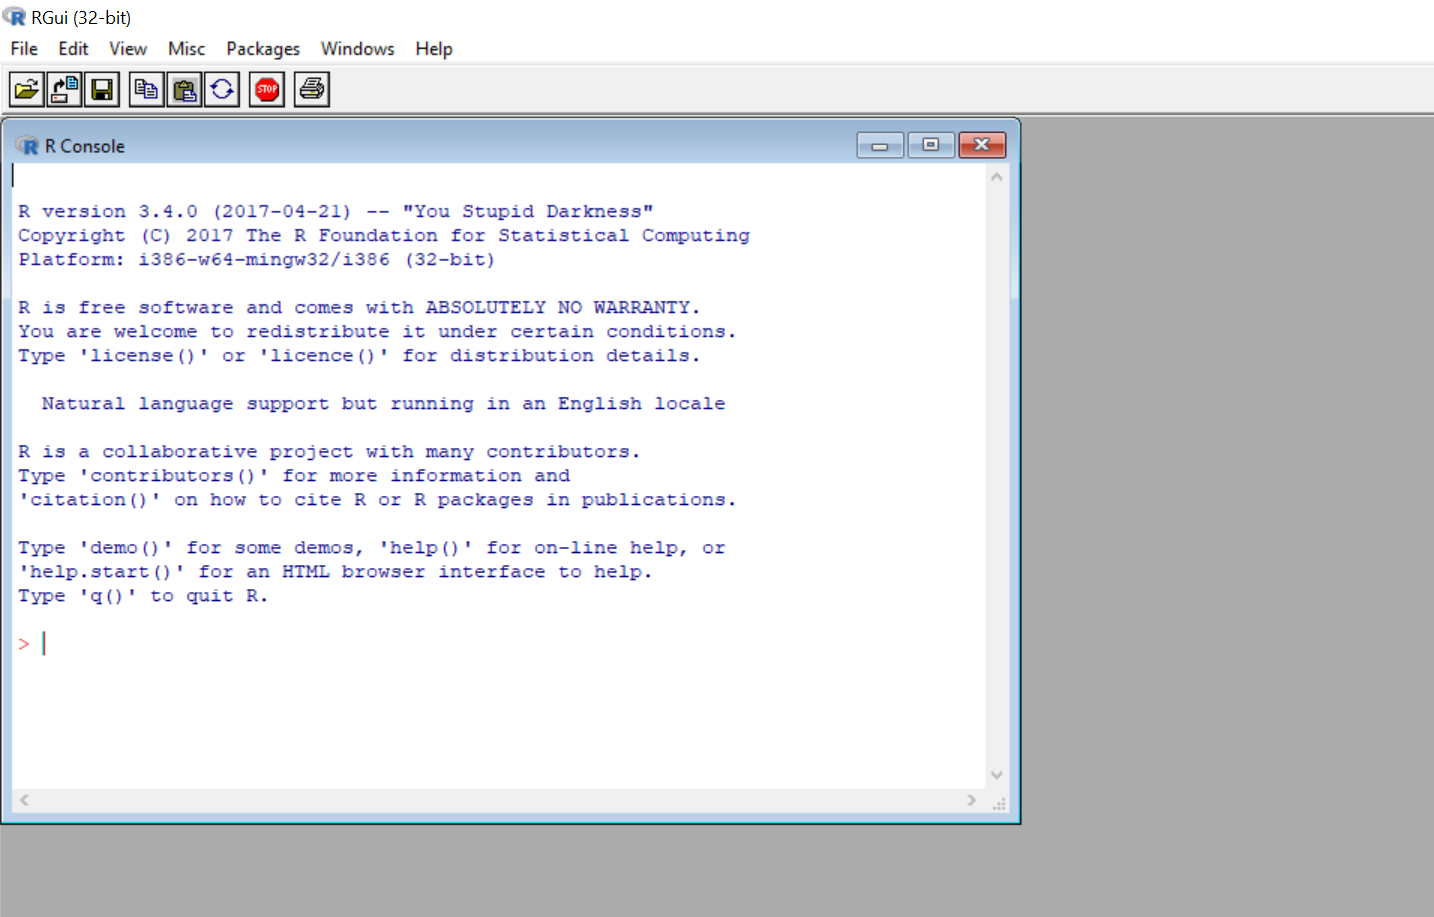
\includegraphics[width=0.7\linewidth]{imagenes/RGui} 

}

\caption{Consola de R}\label{fig:rmark1}
\end{figure}

La \emph{\textbf{consola}} es el corazón de R, allí podemos pedirle cosas y es donde se nos entregan los resultados. También nos avisa de posibles errores (generalmente en color rojo). La consola es lo primero que observamos cuando abrimos el programa. Cuando la consola tiene el cursor \texttt{\textgreater{}} significa que le podemos dar comandos para ejecutar. Si es que tiene el símbolo \texttt{+} quiere decir que nos falta completar el comando anterior.

Un \emph{\textbf{script}} corresponde a una hoja para escribir comandos. Nos sirve para escribir solo los comandos, y cuando seleccionamos y presionamos \emph{\textless Ctrl + R\textgreater{}} (juntos) se ejecuta el comando que hemos escrito y los resultados se visualizaran en la consola Dependiendo del sistema operatio utilizado, la combinación podría ser \textless Ctrl +Enter\textgreater. El script es práctico por que no solo podemos escribir comandos sino también notas personales. Las notas tienen que estar precedidas por el \texttt{\#}.

\hypertarget{r-studio}{%
\section{R Studio}\label{r-studio}}

\href{http://www.rstudio.org}{RStudio} es una interfaz que permite acceder de manera sencilla a todas las funciones de R. Para utilizar RStudio se requiere haber instalado R previamente. La instalación de RStudio se puede realizar desde la \href{http://www.rstudio.org}{página oficial del programa}.

\hypertarget{conociendo-a-rstudio}{%
\subsection{Conociendo a Rstudio}\label{conociendo-a-rstudio}}

Una vez instalados R y RStudio procedemos a ejecutar el programa RStudio desde cualquiera de los iconos que genera y se mostrará la siguiente pantalla:

\begin{figure}

{\centering 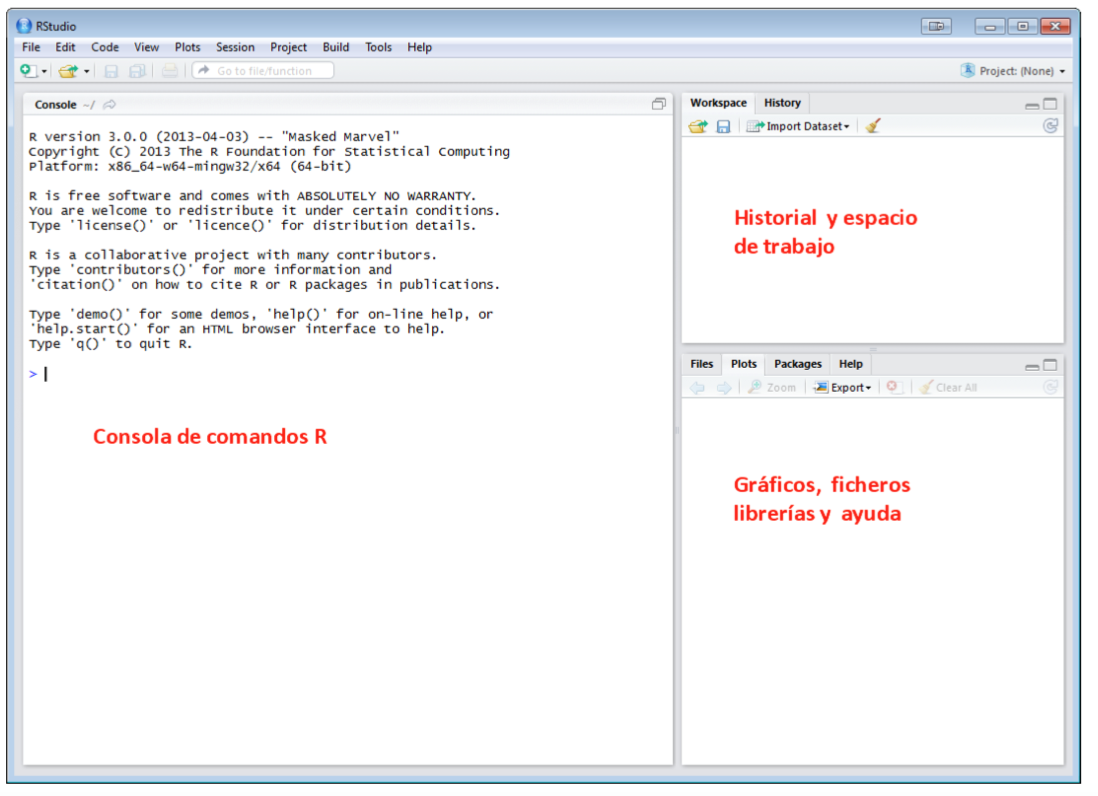
\includegraphics[width=0.7\linewidth]{imagenes/Rstudio} 

}

\caption{Pantalla principal Rstudio}\label{fig:rmark2}
\end{figure}

Esta pantalla está dividida en tres partes:

\begin{enumerate}
\def\labelenumi{\arabic{enumi}.}
\item
  La ventana de la izquierda donde está el prompt \texttt{\textgreater{}} , llamada Consola, es el espacio de trabajo.
\item
  La ventana de la derecha se divide en dos:
\end{enumerate}

\begin{itemize}
\tightlist
\item
  En la ventana superior derecha se encuentra el historial de objetos almacenados en memoria. Desde esta ventana también podemos:\\
\end{itemize}

\begin{enumerate}
\def\labelenumi{\alph{enumi})}
\tightlist
\item
  Limpiar nuestro historial\\
\item
  Importar datos\\
\item
  Muestra los comandos y funciones implementadas de los informes con los que se han trabajado.
\end{enumerate}

\begin{enumerate}
\def\labelenumi{\arabic{enumi}.}
\setcounter{enumi}{2}
\tightlist
\item
  En la ventana inferior de la derecha RStudio muestra el directorio de trabajo, los gráficos que se van generando, paquetes para cargarlos e instalarlos directamente, ayuda y un visor HTML. Estas pestañas se irán describiendo a lo largo del documento
\end{enumerate}

\hypertarget{tipos-de-datos-en-r}{%
\chapter{Tipos de datos en R}\label{tipos-de-datos-en-r}}

\hypertarget{objetos-en-r}{%
\section{Objetos en R}\label{objetos-en-r}}

Hasta ahora nos hemos dedicado a escribir algunas instrucciones para que R las ejecute. A lo largo del curso aprenderemos muchas funciones, sin embargo existen aspectos críticos que debemos saber antes de seguir avanzando.

Lo primero que debemos saber (y que nos evitará que surjan en la consola los nunca agradables errores) es que todos los elementos que maneja R son \textbf{objetos}: un valor numérico es un objeto, un vector es un objeto, una base de datos es un objeto, una función es un objeto, un gráfico es\ldots{} un objeto.

En este laboratorio exploraremos algunos tipos de objetos y sus propiedades básicas para trabajar en R.

\hypertarget{propiedades-de-los-objetos}{%
\subsection{Propiedades de los objetos}\label{propiedades-de-los-objetos}}

\begin{enumerate}
\def\labelenumi{\arabic{enumi}.}
\item
  Los objetos están compuestos por uno o más elementos. Los elementos pueden ser caracteres alfabéticos y/o numéricos. En este curso, los elementos serán considerados datos.
\item
  R guarda los objetos en la memoria activa del ordenador con un nombre especifico. Para ello, asignamos
  un valor a un objeto mediante el uso del operador \texttt{\textless{}-}.
\end{enumerate}

Generemos un objeto de nombre Asignatura que contendrá las palabras \emph{Metodos} y \emph{estadisticos}. En el script de RStudio debemos escribir lo siguiente y luego presionar \textless Ctrl + enter\textgreater:

\begin{Shaded}
\begin{Highlighting}[]
\NormalTok{Asignatura<-}\KeywordTok{c}\NormalTok{(}\StringTok{"Metodos"}\NormalTok{, }\StringTok{"estadisticos"}\NormalTok{)}
\end{Highlighting}
\end{Shaded}

Ahora escribamos \emph{asignatura} y veamos que sucede. En tu script y consola debería aparecer lo siguiente:

\begin{figure}

{\centering 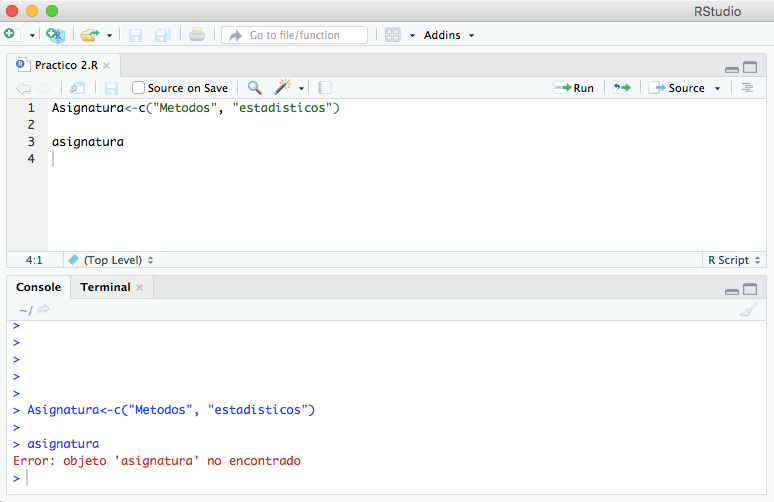
\includegraphics[width=0.7\linewidth]{imagenes/imagen3_asignatura} 

}

\caption{Pantalla principal Rstudio}\label{fig:rmark3}
\end{figure}

Es momento de felicitarnos a nosotros mismos, ya que acabamos de cometer uno de los errores más recurrentes y básicos que se cometen al trabajar en R. ¿Qué fue lo que sucedió?. R discrimina entre letras mayúsculas y minúsculas para el nombre de un objeto, por lo cual no es lo mismo escribir \emph{asignatura} que \emph{Asignatura}.

Ahora escribamos \emph{Asignatura} y veamos que sucede:

\begin{Shaded}
\begin{Highlighting}[]
\NormalTok{Asignatura}
\end{Highlighting}
\end{Shaded}

\begin{verbatim}
## [1] "Metodos"      "estadisticos"
\end{verbatim}

\textbf{IMPORTANTE}: Los datos de caracteres siempre deben estar encerrados entre comillas (\texttt{""}) y los datos son concatenados (combinados) utilizando el comando \texttt{c()}

\hypertarget{tipos-de-objetos}{%
\section{Tipos de Objetos}\label{tipos-de-objetos}}

En este curso nos ocuparemos de aquellos objetos que R utiliza para representar datos: valores, vectores, y dataframes.

\hypertarget{objetos-de-valores-numuxe9ricos}{%
\subsection{Objetos de valores numéricos}\label{objetos-de-valores-numuxe9ricos}}

El objeto mas simple que podemos crear es aquel con contiene solamente un numero real. Generaremos un objeto de nombre \texttt{x} con el valor \texttt{5}:

\begin{Shaded}
\begin{Highlighting}[]
\NormalTok{x<-}\DecValTok{5}
\NormalTok{x}
\end{Highlighting}
\end{Shaded}

\begin{verbatim}
## [1] 5
\end{verbatim}

R permite realizar un sin número de operaciones algebraicas con nuestros objetos. Dichos operaciones
incluyen la adición (\texttt{+}), sustracción (\texttt{-}), multiplicación (\texttt{*}), división (\texttt{/}) y potenciación (\texttt{\^{}}).

\begin{Shaded}
\begin{Highlighting}[]
\CommentTok{# crear objeto a}
\NormalTok{a<-}\DecValTok{15}
\NormalTok{a}
\end{Highlighting}
\end{Shaded}

\begin{verbatim}
## [1] 15
\end{verbatim}

\begin{Shaded}
\begin{Highlighting}[]
\CommentTok{# crear objeto b}
\NormalTok{b<-}\DecValTok{2}
\NormalTok{b}
\end{Highlighting}
\end{Shaded}

\begin{verbatim}
## [1] 2
\end{verbatim}

\begin{Shaded}
\begin{Highlighting}[]
\CommentTok{# sumar a + b}
\NormalTok{a}\OperatorTok{+}\NormalTok{b}
\end{Highlighting}
\end{Shaded}

\begin{verbatim}
## [1] 17
\end{verbatim}

\begin{Shaded}
\begin{Highlighting}[]
\CommentTok{# restar b-a}
\NormalTok{b}\OperatorTok{-}\NormalTok{a}
\end{Highlighting}
\end{Shaded}

\begin{verbatim}
## [1] -13
\end{verbatim}

\begin{Shaded}
\begin{Highlighting}[]
\CommentTok{# restar a - b}
\NormalTok{a}\OperatorTok{-}\NormalTok{b}
\end{Highlighting}
\end{Shaded}

\begin{verbatim}
## [1] 13
\end{verbatim}

\begin{Shaded}
\begin{Highlighting}[]
\CommentTok{# otras operaciones}
\NormalTok{(a}\OperatorTok{+}\NormalTok{b)}\OperatorTok{/}\NormalTok{a}
\end{Highlighting}
\end{Shaded}

\begin{verbatim}
## [1] 1.133333
\end{verbatim}

\begin{Shaded}
\begin{Highlighting}[]
\NormalTok{(a}\OperatorTok{*}\NormalTok{b)}\OperatorTok{/}\NormalTok{(b}\OperatorTok{^}\NormalTok{b)}
\end{Highlighting}
\end{Shaded}

\begin{verbatim}
## [1] 7.5
\end{verbatim}

Otras funciones matemáticas de importancia para nuestro curso son: la raíz cuadrada (\texttt{sqrt}), función
exponencial (\texttt{exp}) y función logarítmica natural (\texttt{log}).

\begin{Shaded}
\begin{Highlighting}[]
\CommentTok{# Raíz cuadrada}
\KeywordTok{sqrt}\NormalTok{(}\DecValTok{9}\NormalTok{)}
\end{Highlighting}
\end{Shaded}

\begin{verbatim}
## [1] 3
\end{verbatim}

\begin{Shaded}
\begin{Highlighting}[]
\CommentTok{# exponencial}
\KeywordTok{exp}\NormalTok{(}\DecValTok{2}\NormalTok{)}
\end{Highlighting}
\end{Shaded}

\begin{verbatim}
## [1] 7.389056
\end{verbatim}

\begin{Shaded}
\begin{Highlighting}[]
\CommentTok{# logaritmo}
\KeywordTok{log}\NormalTok{(}\DecValTok{10}\NormalTok{)}
\end{Highlighting}
\end{Shaded}

\begin{verbatim}
## [1] 2.302585
\end{verbatim}

\hypertarget{vectores}{%
\subsection{Vectores}\label{vectores}}

Un vector representa una secuencia ordenada de elementos (datos) del mismo tipo. Es posible construir vectores de tipo numérico y caracteres. Para nuestros propósitos, los vectores podrán ser considerados como variables.

Generaremos un vector de nombre \texttt{vector1} que contenga tres datos numéricos:

\begin{Shaded}
\begin{Highlighting}[]
\NormalTok{vector1<-}\KeywordTok{c}\NormalTok{(}\DecValTok{1}\NormalTok{,}\DecValTok{5}\NormalTok{,}\DecValTok{7}\NormalTok{)}
\NormalTok{vector1}
\end{Highlighting}
\end{Shaded}

\begin{verbatim}
## [1] 1 5 7
\end{verbatim}

Ahora, generaremos un vector de nombre \texttt{vector2} que contenga tres caracteres:

\begin{Shaded}
\begin{Highlighting}[]
\NormalTok{vector2<-}\KeywordTok{c}\NormalTok{(}\StringTok{"cerezo"}\NormalTok{,}\StringTok{"peral"}\NormalTok{,}\StringTok{"vid"}\NormalTok{) }
\NormalTok{vector2   }
\end{Highlighting}
\end{Shaded}

\begin{verbatim}
## [1] "cerezo" "peral"  "vid"
\end{verbatim}

Intentemos generar un vector de nombre vector3 a partir de los vectores creados:

\textbf{IMPORTANTE}: Los datos son concatenados (combinados) utilizando el comando \texttt{c()}

\hypertarget{funciones-para-generar-vectores}{%
\subsubsection{Funciones para generar vectores}\label{funciones-para-generar-vectores}}

Las funciones \texttt{seq} y \texttt{rep} nos permiten crear patrones de elementos. \texttt{seq} Crea una secuencia de números equiespaciados. Dentro del comando \texttt{seq} el comienzo (\texttt{from}), el fin (\texttt{to}), el espacio entre dos números consecutivos (\texttt{by}) o la cantidad de números en la secuencia (\texttt{length}) pueden ser especificados.

Por ejemplo:

\begin{Shaded}
\begin{Highlighting}[]
\KeywordTok{seq}\NormalTok{(}\DataTypeTok{from=} \DecValTok{2}\NormalTok{, }\DataTypeTok{to=} \DecValTok{8}\NormalTok{, }\DataTypeTok{by=}\DecValTok{2}\NormalTok{)}
\end{Highlighting}
\end{Shaded}

\begin{verbatim}
## [1] 2 4 6 8
\end{verbatim}

\begin{Shaded}
\begin{Highlighting}[]
\KeywordTok{seq}\NormalTok{(}\DataTypeTok{from=}\DecValTok{2}\NormalTok{, }\DataTypeTok{to=} \DecValTok{8}\NormalTok{,}\DataTypeTok{length=}\DecValTok{3}\NormalTok{)}
\end{Highlighting}
\end{Shaded}

\begin{verbatim}
## [1] 2 5 8
\end{verbatim}

Por otra parte, el comando \texttt{rep} repite un elemento (\texttt{x}) una cantidad determinada de veces (\texttt{times}) o hasta lograr una longitud especificada (\texttt{length.out}).

Por ejemplo:

\begin{Shaded}
\begin{Highlighting}[]
\KeywordTok{rep}\NormalTok{ (}\DecValTok{0}\NormalTok{,}\DecValTok{5}\NormalTok{)}
\end{Highlighting}
\end{Shaded}

\begin{verbatim}
## [1] 0 0 0 0 0
\end{verbatim}

\begin{Shaded}
\begin{Highlighting}[]
\KeywordTok{rep}\NormalTok{(}\DecValTok{0}\OperatorTok{:}\DecValTok{2}\NormalTok{,}\DecValTok{3}\NormalTok{)}
\end{Highlighting}
\end{Shaded}

\begin{verbatim}
## [1] 0 1 2 0 1 2 0 1 2
\end{verbatim}

\begin{Shaded}
\begin{Highlighting}[]
\KeywordTok{rep}\NormalTok{(}\DecValTok{1}\OperatorTok{:}\DecValTok{2}\NormalTok{,}\DataTypeTok{length.out=}\DecValTok{7}\NormalTok{)}
\end{Highlighting}
\end{Shaded}

\begin{verbatim}
## [1] 1 2 1 2 1 2 1
\end{verbatim}

\hypertarget{data-frames}{%
\subsection{Data frames}\label{data-frames}}

Un \texttt{data.frame} es un tipo especial de objeto que permite organizar diferentes tipos de vectores
(alfanuméricos). La estructura de un \texttt{data.frame} es muy similar a una hoja de datos, en donde la información
se organiza en filas (observaciones de cada vector) y columnas (vector).

El siguiente ejemplo nos muestra como crear un \texttt{data.frame} llamado \texttt{Notas} a partir de los datos obtenidos de una muestra a 8 alumnos, para cada una de las cuales se ha registrado su edad, género y nota obtenida en la primera prueba parcial del curso Métodos Estadísticos.

Primero, debemos generar los 3 vectores (variables) que utilizaremos para crear nuestro \texttt{data.frame}:

\begin{Shaded}
\begin{Highlighting}[]
\NormalTok{edad <-}\StringTok{ }\KeywordTok{c}\NormalTok{(}\DecValTok{22}\NormalTok{, }\DecValTok{21}\NormalTok{, }\DecValTok{21}\NormalTok{, }\DecValTok{25}\NormalTok{, }\DecValTok{19}\NormalTok{, }\DecValTok{22}\NormalTok{, }\DecValTok{23}\NormalTok{,}\DecValTok{24}\NormalTok{)}
\NormalTok{genero <-}\StringTok{ }\KeywordTok{c}\NormalTok{(}\StringTok{"M"}\NormalTok{,}\StringTok{"F"}\NormalTok{,}\StringTok{"F"}\NormalTok{,}\StringTok{"M"}\NormalTok{,}\StringTok{"M"}\NormalTok{,}\StringTok{"F"}\NormalTok{,}\StringTok{"F"}\NormalTok{,}\StringTok{"M"}\NormalTok{)}
\NormalTok{nota<-}\KeywordTok{c}\NormalTok{(}\FloatTok{3.4}\NormalTok{,}\FloatTok{6.0}\NormalTok{,}\FloatTok{5.1}\NormalTok{,}\FloatTok{4.5}\NormalTok{,}\FloatTok{4.6}\NormalTok{,}\FloatTok{6.1}\NormalTok{,}\FloatTok{4.0}\NormalTok{,}\FloatTok{4.5}\NormalTok{)}
\end{Highlighting}
\end{Shaded}

A continuación, generaremos el \texttt{data.frame} llamado \texttt{Notas}. Es importante tener presente que el lenguaje de R es bastante intuitivo, a tal punto que la función que permite generar un data.frame es \texttt{data.frame\ ()}

\begin{Shaded}
\begin{Highlighting}[]
\NormalTok{Notas <-}\StringTok{ }\KeywordTok{data.frame}\NormalTok{(edad,genero,nota)}
\end{Highlighting}
\end{Shaded}

Un fuerte aplauso para nosotros mismos, acabamos de generar nuestro primer \texttt{data.frame}. Para corroborar si
lo hicimos bien, y al mismo tiempo ver su contenido, simplemente tenemos que llamarlo su nombre:

\begin{Shaded}
\begin{Highlighting}[]
\NormalTok{Notas}
\end{Highlighting}
\end{Shaded}

\begin{verbatim}
##   edad genero nota
## 1   22      M  3.4
## 2   21      F  6.0
## 3   21      F  5.1
## 4   25      M  4.5
## 5   19      M  4.6
## 6   22      F  6.1
## 7   23      F  4.0
## 8   24      M  4.5
\end{verbatim}

En caso de que quisiéramos saber la estructura de nuestro data.frame, podemos utilizar la función:
\texttt{str()}

\begin{Shaded}
\begin{Highlighting}[]
\KeywordTok{str}\NormalTok{(Notas)}
\end{Highlighting}
\end{Shaded}

\begin{verbatim}
## 'data.frame':    8 obs. of  3 variables:
##  $ edad  : num  22 21 21 25 19 22 23 24
##  $ genero: Factor w/ 2 levels "F","M": 2 1 1 2 2 1 1 2
##  $ nota  : num  3.4 6 5.1 4.5 4.6 6.1 4 4.5
\end{verbatim}

R nos acaba de confirmar que Notas es un data.frame de tres variables con 8 observaciones cada una. R
también nos informa además de que dos variables son numéricas y la tercera, el genero, es un factor con dos
valores, ``F'' y ``M''.

En caso de que quisiéramos que R nos entregue el nombre de las variables contenidas en el Notas podemos
utilizar la función \texttt{names()}:

\begin{Shaded}
\begin{Highlighting}[]
\KeywordTok{names}\NormalTok{(Notas)}
\end{Highlighting}
\end{Shaded}

\begin{verbatim}
## [1] "edad"   "genero" "nota"
\end{verbatim}

\hypertarget{valores-perdidos}{%
\subsection{Valores Perdidos}\label{valores-perdidos}}

En algunos casos los elementos que componen un objeto son desconocidos. En estos casos, debemos
especificar que el elemento desconocido se encuentra ``not available'' (\texttt{NA}) , entonces a esa observación le
asignamos el valor especial \texttt{NA}. Es importante tener presente que una operación con elementos \texttt{NA} resulta
\texttt{NA}, ya que por defecto R no incluyen la especificación que omite o remueve las observaciones faltantes.
Para estar seguros de esto, podemos generar un nuevo \texttt{data.frame} llamado \texttt{Notas1} a partir de los datos
obtenidos de una muestra a 8 alumnos.

\begin{Shaded}
\begin{Highlighting}[]
\NormalTok{edad1 <-}\StringTok{ }\KeywordTok{c}\NormalTok{(}\DecValTok{22}\NormalTok{, }\DecValTok{21}\NormalTok{, }\DecValTok{21}\NormalTok{, }\DecValTok{25}\NormalTok{, }\DecValTok{19}\NormalTok{, }\DecValTok{22}\NormalTok{, }\DecValTok{23}\NormalTok{,}\DecValTok{24}\NormalTok{)}
\NormalTok{genero1 <-}\StringTok{ }\KeywordTok{c}\NormalTok{(}\StringTok{"M"}\NormalTok{,}\StringTok{"F"}\NormalTok{,}\StringTok{"F"}\NormalTok{,}\StringTok{"M"}\NormalTok{,}\StringTok{"M"}\NormalTok{,}\StringTok{"F"}\NormalTok{,}\StringTok{"F"}\NormalTok{,}\StringTok{"M"}\NormalTok{)}
\NormalTok{nota1<-}\KeywordTok{c}\NormalTok{(}\FloatTok{3.4}\NormalTok{,}\FloatTok{6.0}\NormalTok{,}\FloatTok{5.1}\NormalTok{,}\FloatTok{4.5}\NormalTok{,}\FloatTok{4.6}\NormalTok{,}\FloatTok{6.1}\NormalTok{,}\FloatTok{4.0}\NormalTok{,}\OtherTok{NA}\NormalTok{)}
\NormalTok{Notas1 <-}\StringTok{ }\KeywordTok{data.frame}\NormalTok{(edad1,genero1,nota1)}
\end{Highlighting}
\end{Shaded}

Apliquemos una operación básica a la información contenida en Notas1. Podemos estimar la nota promedio
de los 8 alumnos, para ello utilizaremos la función \texttt{mean()}, la cual exploraremos más adelante en nuestro
curso:

\begin{Shaded}
\begin{Highlighting}[]
\KeywordTok{mean}\NormalTok{(Notas1}\OperatorTok{$}\NormalTok{nota1)}
\end{Highlighting}
\end{Shaded}

\begin{verbatim}
## [1] NA
\end{verbatim}

Lo que obtuvimos como resultado fue \texttt{NA}. Esto se debe a que no le especificamos a R que debe omitir los
NAs en nuestro data.frame. Una forma de solucionar este problema es utilizar la operación \texttt{na.rm=TRUE}, la
cual especifica que la operación se efectué con los datos válidos excluyendo los NAs:

\begin{Shaded}
\begin{Highlighting}[]
\KeywordTok{mean}\NormalTok{(Notas1}\OperatorTok{$}\NormalTok{nota1, }\DataTypeTok{na.rm=}\OtherTok{TRUE}\NormalTok{)}
\end{Highlighting}
\end{Shaded}

\begin{verbatim}
## [1] 4.814286
\end{verbatim}

Magia! Con una simple orden acabamos de solucionar un simple pero doloroso problema.

\hypertarget{lectura-y-manipulaciuxf3n-de-datos-en-rstudio}{%
\chapter{Lectura y manipulación de datos en RStudio}\label{lectura-y-manipulaciuxf3n-de-datos-en-rstudio}}

Hoy en día la información generada a partir del mundo natural se multiplica minuto a minuto. Desde un punto de vista académico y/o profesional, la correcta toma de decisiones demandará la recolección y manejo de grandes cantidades de datos, los cuales nos permitirán describir y determinar propiedades del mundo natural.

Una base de datos se puede definir como un conjunto de información perteneciente a un mismo contexto y almacenada sistemáticamente para su posterior uso. Cada base de datos se compone de una tablas que guarda un conjunto de datos. Cada tabla tiene una o más columnas y filas.

En este laboratorio comenzaremos a trabajar con bases de datos. Para ello abordaremos cuatro tópicos centrales:

\begin{enumerate}
\def\labelenumi{\arabic{enumi}.}
\tightlist
\item
  La preparación de los datos para poder trabajarlos en R,
\item
  La importación de una base de datos a R,
\item
  La edición de los datos contenidos en la base de datos,
\item
  La exploración de la información contenida en nuestra base de datos.
\end{enumerate}

\hypertarget{preparemos-los-datos-para-r}{%
\section{Preparemos los datos para R}\label{preparemos-los-datos-para-r}}

Al mencionar que trabajaremos con base de datos, inmediatamente surge el desafío de como podemos ingresar nuestra información a R. Lo primero que debemos tener presente es que a R ``le encantan'' las bases de datos que tienen cada observación en una fila y que en cada columna incorpora una variable. Por ejemplo, si tenemos una base de datos con la altura y género de los alumnos del curso ``métodos estadísticos'' de la escuela de Agronomía, esta se vería de la siguiente manera en excel:

\begin{figure}

{\centering 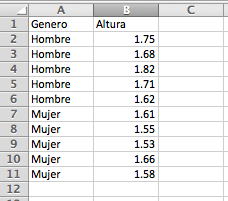
\includegraphics[width=0.4\linewidth]{imagenes/fig4_basedatos} 

}

\caption{Ejemplo de base de datos en excel}\label{fig:rmark4}
\end{figure}

Si creáramaos esta misma base de datos en Rstudio deberíamos hacer lo siguiente:

\begin{Shaded}
\begin{Highlighting}[]
\NormalTok{genero <-}\StringTok{ }\KeywordTok{c}\NormalTok{(}\StringTok{"Hombre"}\NormalTok{,}\StringTok{"Hombre"}\NormalTok{,}\StringTok{"Hombre"}\NormalTok{,}\StringTok{"Hombre"}\NormalTok{,}\StringTok{"Hombre"}\NormalTok{,}\StringTok{"Mujer"}\NormalTok{,}\StringTok{"Mujer"}\NormalTok{,}\StringTok{"Mujer"}\NormalTok{,}\StringTok{"Mujer"}\NormalTok{,}\StringTok{"Mujer"}\NormalTok{)}
\NormalTok{altura<-}\KeywordTok{c}\NormalTok{(}\FloatTok{1.75}\NormalTok{,}\FloatTok{1.68}\NormalTok{,}\FloatTok{1.82}\NormalTok{,}\FloatTok{1.71}\NormalTok{,}\FloatTok{1.62}\NormalTok{,}\FloatTok{1.61}\NormalTok{,}\FloatTok{1.55}\NormalTok{,}\FloatTok{1.53}\NormalTok{,}\FloatTok{1.66}\NormalTok{,}\FloatTok{1.58}\NormalTok{)}
\NormalTok{base_de_datos <-}\StringTok{ }\KeywordTok{data.frame}\NormalTok{(genero,altura)}
\end{Highlighting}
\end{Shaded}

¿Cuáles son las dimensiones de esta base de datos?. La tabla tiene una dimensión de 10x2. Esto quiere decir que está compuesta de diez filas y dos columnas.

\textbf{IMPORTANTE:}

\begin{itemize}
\item
  Las filas contienen nuestras observaciones.
\item
  Las columnas contienen nuestras variables.
\item
  R reconoce puntos (``.'') y no comas (``,'') como separador de decimales.
\item
  Revisar que nuestra base de datos no contenga filas en blanco (sin valores). Cuando eso ocurra se recomienda rellenar el espacio con las letras \texttt{NA} (``Not available'').
\end{itemize}

\hypertarget{quuxe9-formato-de-archivos-reconoce-r}{%
\subsection{¿Qué formato de archivos reconoce R?}\label{quuxe9-formato-de-archivos-reconoce-r}}

R es muy versátil para reconocer y leer múltiples formatos de archivo. Los archivos de texto plano, tales
como TXT o CSV, son la opción más sencilla para importar datos desde hojas de cálculo. Por ejemplo, Excel
permite guardar archivos .txt (texto delimitado por tabulaciones) o .csv (texto delimitados por comas). En
este curso los alentamos a utilizar el formato CSV. Una ventaja de este tipo de representación es que los
datos se pueden visualizar/editar con un editor de texto. CSV representa la información en forma de tabla
donde las columnas se delimitan con un carácter (por defecto, con coma)* y las filas con saltos de línea.

\hypertarget{importemos-los-datos-a-r}{%
\section{Importemos los datos a R}\label{importemos-los-datos-a-r}}

Para importar los datos, necesitamos especificar a R la localización (ruta) de los datos en el computador. El
problema es que la ruta de los archivos generalmente son muy largas y difícil de memorizar. Además, si se
equivocan al escribirla, R no la reconocerá. Es por ello que es preferible que RStudio haga ese difícil trabajo.

A lo largo de nuestro curso, el método que utilizaremos para importar la base de datos se basará en la
herramienta Import dataset. Rstudio proporciona una función de importación a través de la pestaña Import
dataset en la parte superior derecha.

\begin{figure}

{\centering 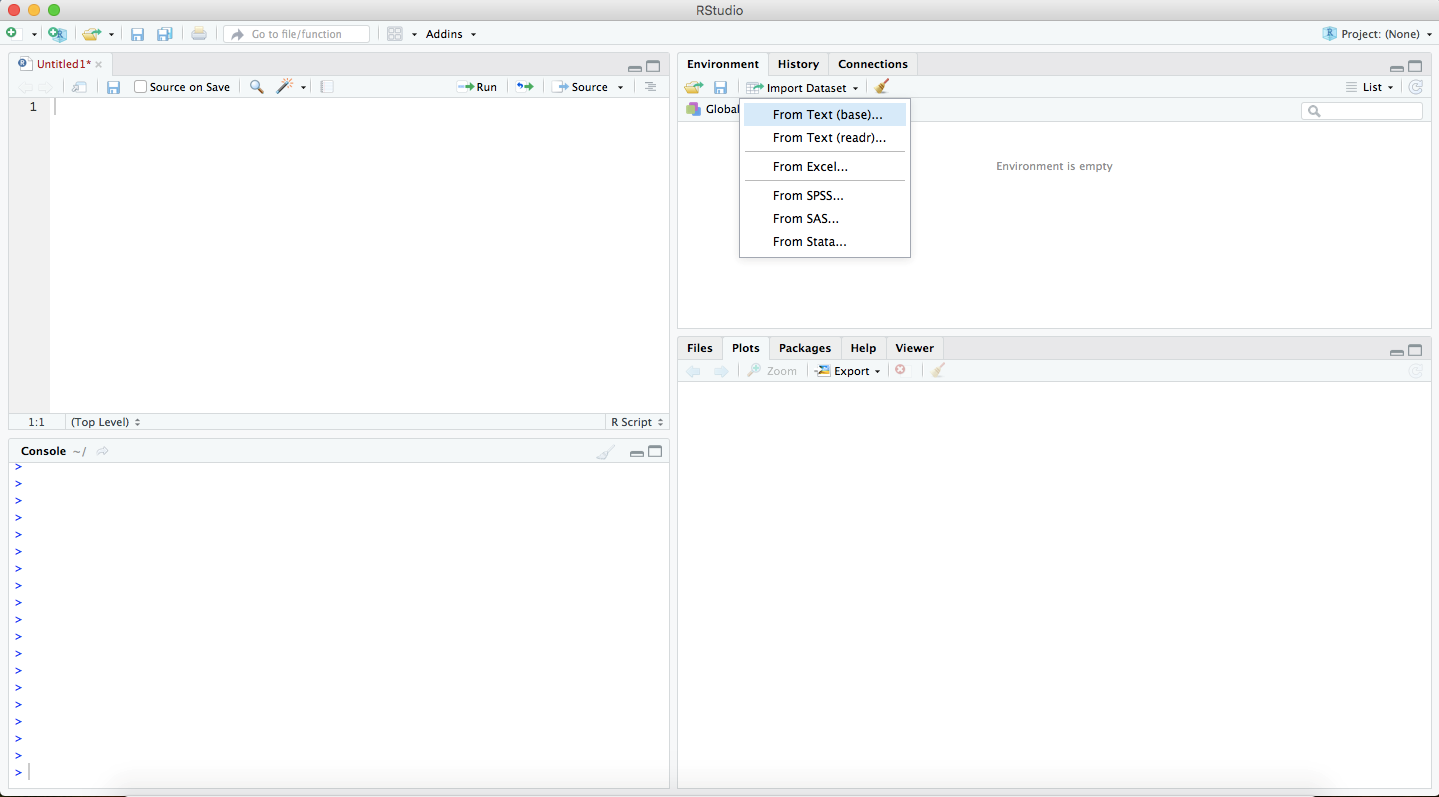
\includegraphics[width=0.8\linewidth]{imagenes/fig5_imp_datos} 

}

\caption{Importación de datos desde Rstudio}\label{fig:rmark5}
\end{figure}

Esta función nos permitirá buscar el archivo de datos, seleccionarlo y finalmente para poder cargar la base de
datos en R. Al seleccionar la opción From Text (base), podemos navegar en nuestro computador para
encontrar nuestro archivo con la base de datos. Una vez lo seleccionamos, solamente debemos hacer clic en
el botón Open para que la magia se haga realidad.

\begin{itemize}
\tightlist
\item
  Para aprender sobre otros métodos de importación de datos les sugerimos visitar el siguiente \href{https://thepracticalr.wordpress.com/2016/09/23/importing-data-into-r/}{link}
\end{itemize}

Una vez seleccionado el archivo, se abrirá una ventana que entrega una vista preliminar del archivo
seleccionado. En la parte superior izquierda, podrán observar la opción name, la cual nos permite asignar un
nombre a nuestra base de datos (¿Recuerdan el comando \texttt{\textless{}-}?). En este caso, nuestra base de datos recibirá
el nombre \texttt{data}. Lo único que resta por hacer es darle la orden a R para que importe la base de datos. Esto lo
lo podemos hacer habiendo clic en el botón \texttt{Import}.

\begin{figure}

{\centering 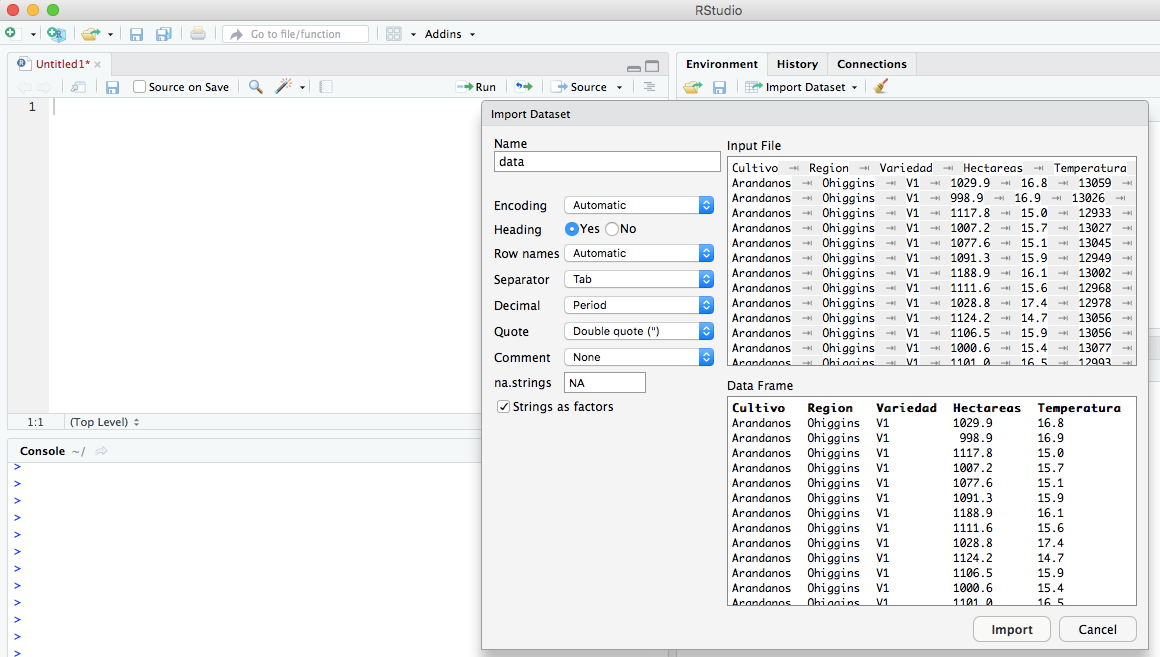
\includegraphics[width=0.8\linewidth]{imagenes/fig5_import} 

}

\caption{Paso final para Importación de datos}\label{fig:rmark6}
\end{figure}

La base de datos que trabajaremos a lo largo del curso contiene nueve diferentes variables:

\begin{enumerate}
\def\labelenumi{\arabic{enumi}.}
\item
  \textbf{Cultivo}: Proporciona el cultivo sobre el cuales realizaron las observaciones.
\item
  \textbf{Region}: Hace referencia a la división territorial de Chile en donde se realizó el muestreo.
\item
  \textbf{Variedad}: Indica las diferentes variedades del cultivo que fueron estudiadas.
\item
  \textbf{Hectareas}: Proporciona la superficie plantada con el cultivo (hectáreas).
\item
  \textbf{Temperatura}: Indica el valor de temperatura ambiental promedio anual para cada sitio de muestreo.
\item
  \textbf{costo\_jh}: Indica el valor pagado por jornada hombre (pesos chilenos).
\item
  \textbf{rendimiento}: Proporciona el rendimiento del cultivo en cada sitio de muestreo (toneladas/hectárea).
\item
  \textbf{Perdida\_plaga}: Indica las perdidas en rendimiento causadas por la presencia de insectos plaga (porcentaje).
\item
  \textbf{mano\_de\_obra}: Proporciona el número de personas contratadas para realizar las labores asociadas a la temporada de cosecha en cada sitio de muestreo.
\end{enumerate}

\textbf{Importante:}

\begin{itemize}
\tightlist
\item
  La base de datos acá presentada es una base de datos ficticia creada sólo con fines académicos
\end{itemize}

\hypertarget{exploremos-los-datos-a-r}{%
\section{Exploremos los datos a R}\label{exploremos-los-datos-a-r}}

Al importar nuestro archivo, lo que buscamos es analizar incluso graficar la información contenida en la
base de datos. Sin embargo, antes de eso existe un paso sensible y crítico que jamás debemos olvidar. Es
importante asegurarnos que importamos correctamente nuestros datos!

La función \texttt{str()} nos mostrará el tipo de datos contenido en nuestra base de datos y enumerará cada variable
de columna junto con su tipo de datos.

\begin{Shaded}
\begin{Highlighting}[]
\KeywordTok{str}\NormalTok{(data)}
\end{Highlighting}
\end{Shaded}

\begin{verbatim}
## 'data.frame':    120 obs. of  9 variables:
##  $ Cultivo      : Factor w/ 1 level "Arandanos": 1 1 1 1 1 1 1 1 1 1 ...
##  $ Region       : Factor w/ 4 levels "BioBio","La_Araucania",..: 4 4 4 4 4 4 4 4 4 4 ...
##  $ Variedad     : Factor w/ 2 levels "V1","V2": 1 1 1 1 1 1 1 1 1 1 ...
##  $ Hectareas    : num  1030 999 1118 1007 1078 ...
##  $ Temperatura  : num  16.8 16.9 15 15.7 15.1 15.9 16.1 15.6 17.4 14.7 ...
##  $ costo_jh     : int  13059 13026 12933 13027 13045 12949 13002 12968 12978 13056 ...
##  $ rendimiento  : num  6866 7122 7041 6892 6928 ...
##  $ Perdida_plaga: num  35.1 34.3 31.7 40.5 35.6 33 38.1 37.9 34.8 34.4 ...
##  $ mano_de_obra : int  3080 2728 3120 3135 3276 2966 2725 2874 2785 3193 ...
\end{verbatim}

Como podemos ver, nuestra base contiene variables con diferentes tipos de datos.

La función \texttt{summary()} nos proporciona para cada variable un conjunto de estadísticas descriptivas, según el tipo de variable:

\begin{Shaded}
\begin{Highlighting}[]
\KeywordTok{summary}\NormalTok{(data)}
\end{Highlighting}
\end{Shaded}

\begin{verbatim}
##       Cultivo             Region   Variedad   Hectareas     
##  Arandanos:120   BioBio      :30   V1:60    Min.   : 998.9  
##                  La_Araucania:30   V2:60    1st Qu.:1477.7  
##                  Maule       :30            Median :1797.0  
##                  Ohiggins    :30            Mean   :2090.7  
##                                             3rd Qu.:2352.7  
##                                             Max.   :3788.0  
##   Temperatura       costo_jh      rendimiento   Perdida_plaga  
##  Min.   :10.00   Min.   :11893   Min.   :4166   Min.   :24.70  
##  1st Qu.:12.50   1st Qu.:11997   1st Qu.:4765   1st Qu.:32.95  
##  Median :13.75   Median :12490   Median :5457   Median :34.60  
##  Mean   :13.74   Mean   :12500   Mean   :5617   Mean   :34.66  
##  3rd Qu.:15.10   3rd Qu.:13002   3rd Qu.:6285   3rd Qu.:37.30  
##  Max.   :17.40   Max.   :13121   Max.   :7247   Max.   :42.80  
##   mano_de_obra 
##  Min.   :2609  
##  1st Qu.:3092  
##  Median :3312  
##  Mean   :3384  
##  3rd Qu.:3645  
##  Max.   :4274
\end{verbatim}

\begin{enumerate}
\def\labelenumi{\arabic{enumi}.}
\item
  \textbf{Variables numéricas:} \texttt{summary()} proporciona el rango, los cuartiles, la mediana y la media.
\item
  \textbf{Variables factoriales:} \texttt{summary()} proporciona una tabla con frecuencias.
\item
  \textbf{Variables numéricas y factoriales:} \texttt{summary()}, en caso de que existan, nos entregará información sobre el número de valores faltantes (\texttt{NAs}).
\item
  \textbf{Variables de caracteres:} \texttt{summary()} solo proporciona la longitud de la variable.
\end{enumerate}

La función \texttt{head()} nos entregará las primeras filas de nuestra base de datos. Por defecto serán las primeras 6:

\begin{Shaded}
\begin{Highlighting}[]
\KeywordTok{head}\NormalTok{(data)}
\end{Highlighting}
\end{Shaded}

\begin{verbatim}
##     Cultivo   Region Variedad Hectareas Temperatura costo_jh rendimiento
## 1 Arandanos Ohiggins       V1    1029.9        16.8    13059      6866.5
## 2 Arandanos Ohiggins       V1     998.9        16.9    13026      7122.1
## 3 Arandanos Ohiggins       V1    1117.8        15.0    12933      7041.2
## 4 Arandanos Ohiggins       V1    1007.2        15.7    13027      6891.5
## 5 Arandanos Ohiggins       V1    1077.6        15.1    13045      6927.7
## 6 Arandanos Ohiggins       V1    1091.3        15.9    12949      6900.4
##   Perdida_plaga mano_de_obra
## 1          35.1         3080
## 2          34.3         2728
## 3          31.7         3120
## 4          40.5         3135
## 5          35.6         3276
## 6          33.0         2966
\end{verbatim}

En caso de que quisiéramos ampliar el número de filas:

\begin{Shaded}
\begin{Highlighting}[]
\KeywordTok{head}\NormalTok{(data, }\DecValTok{10}\NormalTok{)}
\end{Highlighting}
\end{Shaded}

\begin{verbatim}
##      Cultivo   Region Variedad Hectareas Temperatura costo_jh rendimiento
## 1  Arandanos Ohiggins       V1    1029.9        16.8    13059      6866.5
## 2  Arandanos Ohiggins       V1     998.9        16.9    13026      7122.1
## 3  Arandanos Ohiggins       V1    1117.8        15.0    12933      7041.2
## 4  Arandanos Ohiggins       V1    1007.2        15.7    13027      6891.5
## 5  Arandanos Ohiggins       V1    1077.6        15.1    13045      6927.7
## 6  Arandanos Ohiggins       V1    1091.3        15.9    12949      6900.4
## 7  Arandanos Ohiggins       V1    1188.9        16.1    13002      6943.9
## 8  Arandanos Ohiggins       V1    1111.6        15.6    12968      6885.7
## 9  Arandanos Ohiggins       V1    1028.8        17.4    12978      6724.3
## 10 Arandanos Ohiggins       V1    1124.2        14.7    13056      6920.4
##    Perdida_plaga mano_de_obra
## 1           35.1         3080
## 2           34.3         2728
## 3           31.7         3120
## 4           40.5         3135
## 5           35.6         3276
## 6           33.0         2966
## 7           38.1         2725
## 8           37.9         2874
## 9           34.8         2785
## 10          34.4         3193
\end{verbatim}

Por otro lado, la función \texttt{tail()} nos entregará las últimas filas de nuestra base de datos. Por defecto serán
las últimas 6:

\begin{Shaded}
\begin{Highlighting}[]
\KeywordTok{tail}\NormalTok{(data)}
\end{Highlighting}
\end{Shaded}

\begin{verbatim}
##       Cultivo       Region Variedad Hectareas Temperatura costo_jh
## 115 Arandanos La_Araucania       V2    1857.6        11.1    11974
## 116 Arandanos La_Araucania       V2    1862.7        11.6    11960
## 117 Arandanos La_Araucania       V2    1894.5        10.6    12023
## 118 Arandanos La_Araucania       V2    1873.5        11.1    11971
## 119 Arandanos La_Araucania       V2    1915.4        11.5    12065
## 120 Arandanos La_Araucania       V2    1932.1        13.5    12084
##     rendimiento Perdida_plaga mano_de_obra
## 115      4591.7          33.2         3439
## 116      4689.4          38.1         3566
## 117      4400.5          24.7         3552
## 118      4380.6          37.6         3449
## 119      4424.1          35.1         3550
## 120      4331.0          38.3         3162
\end{verbatim}

La función \texttt{names()} nos entregará el nombre de las variables (columnas) contenidas en nuestra base de
datos:

\begin{Shaded}
\begin{Highlighting}[]
\KeywordTok{names}\NormalTok{(data)}
\end{Highlighting}
\end{Shaded}

\begin{verbatim}
## [1] "Cultivo"       "Region"        "Variedad"      "Hectareas"    
## [5] "Temperatura"   "costo_jh"      "rendimiento"   "Perdida_plaga"
## [9] "mano_de_obra"
\end{verbatim}

En caso de que quisiéramos conocer las dimensiones (número de columnas y filas) de nuestra base de datos,
podemos utilizar la función \texttt{dim()}:

\begin{Shaded}
\begin{Highlighting}[]
\KeywordTok{dim}\NormalTok{(data)}
\end{Highlighting}
\end{Shaded}

\begin{verbatim}
## [1] 120   9
\end{verbatim}

\textbf{Tips:}

Mucho de lo anteriormente visto lo podemos transformar en tablas mucho más amigables con la función \texttt{ktable} del paquete \texttt{knitr}. Por ejemplo la siguiente Tabla se obtuvo mediante el siguiente código:

\begin{Shaded}
\begin{Highlighting}[]
\NormalTok{knitr}\OperatorTok{::}\KeywordTok{kable}\NormalTok{(}
  \KeywordTok{head}\NormalTok{(data), }
  \DataTypeTok{caption =} \StringTok{"Ejemplo de Tabla de Datos con ktable"}\NormalTok{)}
\end{Highlighting}
\end{Shaded}

\begin{table}[t]

\caption{\label{tab:unnamed-chunk-10}Ejemplo de Tabla de Datos con ktable}
\centering
\begin{tabular}{l|l|l|r|r|r|r|r|r}
\hline
Cultivo & Region & Variedad & Hectareas & Temperatura & costo\_jh & rendimiento & Perdida\_plaga & mano\_de\_obra\\
\hline
Arandanos & Ohiggins & V1 & 1029.9 & 16.8 & 13059 & 6866.5 & 35.1 & 3080\\
\hline
Arandanos & Ohiggins & V1 & 998.9 & 16.9 & 13026 & 7122.1 & 34.3 & 2728\\
\hline
Arandanos & Ohiggins & V1 & 1117.8 & 15.0 & 12933 & 7041.2 & 31.7 & 3120\\
\hline
Arandanos & Ohiggins & V1 & 1007.2 & 15.7 & 13027 & 6891.5 & 40.5 & 3135\\
\hline
Arandanos & Ohiggins & V1 & 1077.6 & 15.1 & 13045 & 6927.7 & 35.6 & 3276\\
\hline
Arandanos & Ohiggins & V1 & 1091.3 & 15.9 & 12949 & 6900.4 & 33.0 & 2966\\
\hline
\end{tabular}
\end{table}

\hypertarget{exploremos-los-datos-r-con-la-libreria-dplyr}{%
\section{Exploremos los datos R con la libreria dplyr}\label{exploremos-los-datos-r-con-la-libreria-dplyr}}

Una de las grandes ventajas de R es la ampliación de sus funcionalidades básicas mediante paquetes
(packages) o librerías. Las librerías de R se pueden instalar de múltiples formas. En RStudio, lo haremos de
siguiendo una serie de sencillos pasos.

Debemos hacer clic en la pestaña package ubicada en el panel inferior derecho. Al hacer clic en esta pestaña,
aparecerá una pequeña ventana con tres campos principales: Install from, packages, and Install to Library.
Solo necesitamos preocuparnos por el campo packages, los otros dos los dejaremos en su valor
predeterminado.

\begin{figure}

{\centering 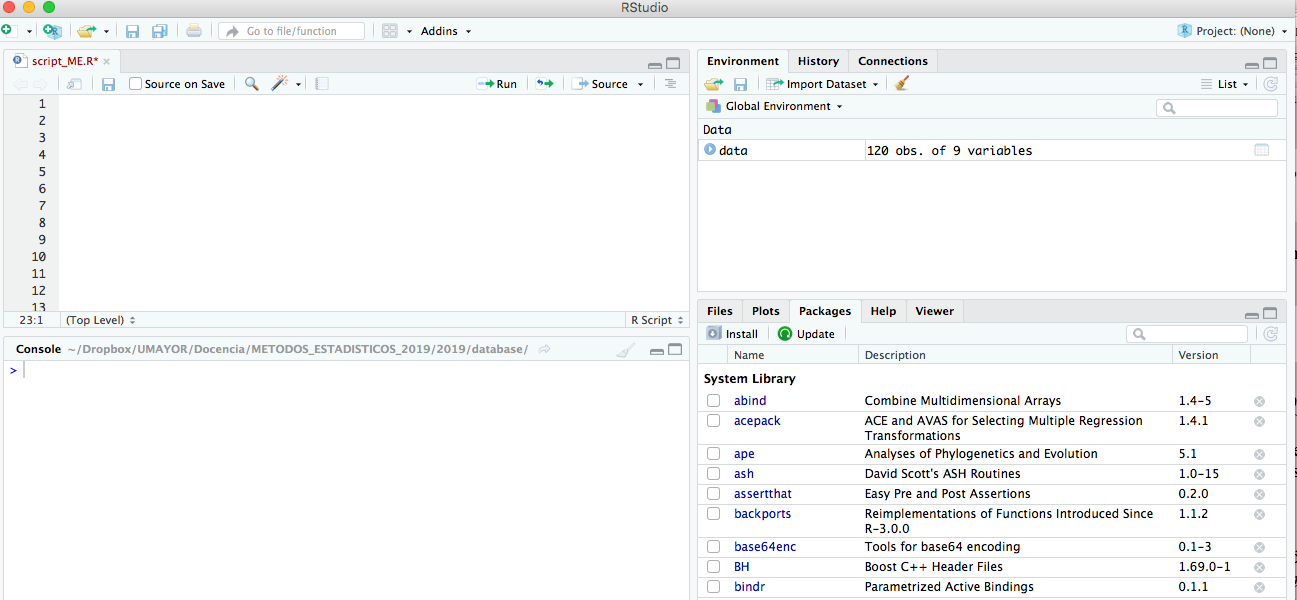
\includegraphics[width=0.8\linewidth]{imagenes/fig7_dplyr} 

}

\caption{Instalación de paquete dplyr}\label{fig:rmark7}
\end{figure}

Ahora, al escribir las primeras letras del nombre de una librería (en este caso \texttt{dplyr}), Rstudio proporcionará
una lista de librerías disponibles que coincidan con esta palabra. Después de encontrar la librería, todo lo
que tenemos que hacer es hacer clic en el botón Install y dejar que Rstudio trabaje.

\begin{figure}

{\centering 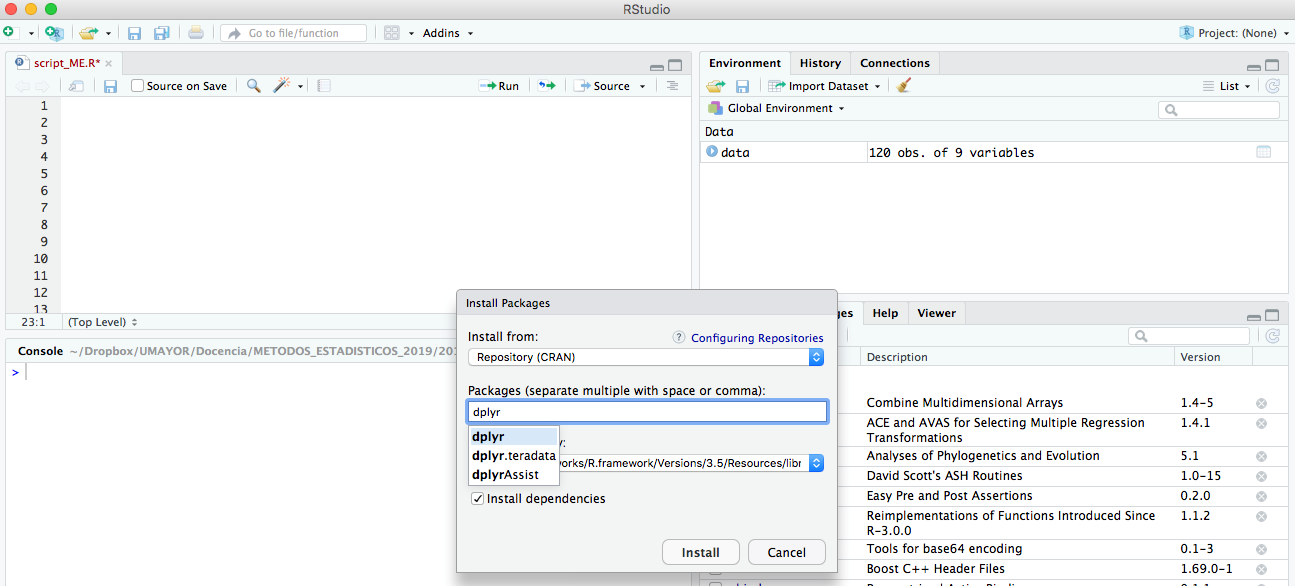
\includegraphics[width=0.8\linewidth]{imagenes/fig8_dplyr} 

}

\caption{Instalación de paquete dplyr (2do paso)}\label{fig:rmark8}
\end{figure}

A pesar de estar instalada, a menos que lo especifiquemos, R no cargará la librería en la consola. Entonces,
debemos ``llamar'' a la librería que acabamos de instalar con el comando \texttt{library(dplyr)}.

\begin{Shaded}
\begin{Highlighting}[]
\KeywordTok{library}\NormalTok{(dplyr)}
\end{Highlighting}
\end{Shaded}

La librería dplyr incluye un conjunto de comandos que coinciden con las acciones más comunes que se
realizan sobre un conjunto de datos (seleccionar filas \texttt{filter}, seleccionar columnas \texttt{select}, resumir mediante
alguna medida numérica \texttt{summarise}, entre muchas otras). Para mayor información sobre la librería dplyr
puedes acceder al siguiente \href{https://rpubs.com/joser/dplyr}{link}.

La función \texttt{select()} selecciona columnas de nuestra base:

Intentemos seleccionar la columna Region en la base de datos llamada data

\begin{Shaded}
\begin{Highlighting}[]
\KeywordTok{select}\NormalTok{(data, Region)}
\end{Highlighting}
\end{Shaded}

\begin{verbatim}
##           Region
## 1       Ohiggins
## 2       Ohiggins
## 3       Ohiggins
## 4       Ohiggins
## 5       Ohiggins
## 6       Ohiggins
## 7       Ohiggins
## 8       Ohiggins
## 9       Ohiggins
## 10      Ohiggins
## 11      Ohiggins
## 12      Ohiggins
## 13      Ohiggins
## 14      Ohiggins
## 15      Ohiggins
## 16      Ohiggins
## 17      Ohiggins
## 18      Ohiggins
## 19      Ohiggins
## 20      Ohiggins
## 21      Ohiggins
## 22      Ohiggins
## 23      Ohiggins
## 24      Ohiggins
## 25      Ohiggins
## 26      Ohiggins
## 27      Ohiggins
## 28      Ohiggins
## 29      Ohiggins
## 30      Ohiggins
## 31         Maule
## 32         Maule
## 33         Maule
## 34         Maule
## 35         Maule
## 36         Maule
## 37         Maule
## 38         Maule
## 39         Maule
## 40         Maule
## 41         Maule
## 42         Maule
## 43         Maule
## 44         Maule
## 45         Maule
## 46         Maule
## 47         Maule
## 48         Maule
## 49         Maule
## 50         Maule
## 51         Maule
## 52         Maule
## 53         Maule
## 54         Maule
## 55         Maule
## 56         Maule
## 57         Maule
## 58         Maule
## 59         Maule
## 60         Maule
## 61        BioBio
## 62        BioBio
## 63        BioBio
## 64        BioBio
## 65        BioBio
## 66        BioBio
## 67        BioBio
## 68        BioBio
## 69        BioBio
## 70        BioBio
## 71        BioBio
## 72        BioBio
## 73        BioBio
## 74        BioBio
## 75        BioBio
## 76        BioBio
## 77        BioBio
## 78        BioBio
## 79        BioBio
## 80        BioBio
## 81        BioBio
## 82        BioBio
## 83        BioBio
## 84        BioBio
## 85        BioBio
## 86        BioBio
## 87        BioBio
## 88        BioBio
## 89        BioBio
## 90        BioBio
## 91  La_Araucania
## 92  La_Araucania
## 93  La_Araucania
## 94  La_Araucania
## 95  La_Araucania
## 96  La_Araucania
## 97  La_Araucania
## 98  La_Araucania
## 99  La_Araucania
## 100 La_Araucania
## 101 La_Araucania
## 102 La_Araucania
## 103 La_Araucania
## 104 La_Araucania
## 105 La_Araucania
## 106 La_Araucania
## 107 La_Araucania
## 108 La_Araucania
## 109 La_Araucania
## 110 La_Araucania
## 111 La_Araucania
## 112 La_Araucania
## 113 La_Araucania
## 114 La_Araucania
## 115 La_Araucania
## 116 La_Araucania
## 117 La_Araucania
## 118 La_Araucania
## 119 La_Araucania
## 120 La_Araucania
\end{verbatim}

La función \texttt{select()} también nos permite seleccionar todas las columnas excepto una:

\begin{Shaded}
\begin{Highlighting}[]
\KeywordTok{select}\NormalTok{(data, }\OperatorTok{-}\NormalTok{Region)}
\end{Highlighting}
\end{Shaded}

\begin{verbatim}
##       Cultivo Variedad Hectareas Temperatura costo_jh rendimiento
## 1   Arandanos       V1    1029.9        16.8    13059      6866.5
## 2   Arandanos       V1     998.9        16.9    13026      7122.1
## 3   Arandanos       V1    1117.8        15.0    12933      7041.2
## 4   Arandanos       V1    1007.2        15.7    13027      6891.5
## 5   Arandanos       V1    1077.6        15.1    13045      6927.7
## 6   Arandanos       V1    1091.3        15.9    12949      6900.4
## 7   Arandanos       V1    1188.9        16.1    13002      6943.9
## 8   Arandanos       V1    1111.6        15.6    12968      6885.7
## 9   Arandanos       V1    1028.8        17.4    12978      6724.3
## 10  Arandanos       V1    1124.2        14.7    13056      6920.4
## 11  Arandanos       V1    1106.5        15.9    13056      7056.9
## 12  Arandanos       V1    1000.6        15.4    13077      6898.6
## 13  Arandanos       V1    1101.0        16.5    12993      6797.2
## 14  Arandanos       V1    1113.9        14.0    12975      6858.2
## 15  Arandanos       V1    1159.9        14.7    13003      7064.3
## 16  Arandanos       V2    1110.8        14.3    12970      7028.4
## 17  Arandanos       V2    1091.4        13.7    13003      7127.7
## 18  Arandanos       V2    1173.8        15.7    12994      7247.3
## 19  Arandanos       V2    1034.9        15.1    13033      6896.8
## 20  Arandanos       V2    1081.7        14.3    13107      6927.3
## 21  Arandanos       V2    1120.4        14.8    13013      6893.3
## 22  Arandanos       V2    1054.0        16.9    12998      6929.0
## 23  Arandanos       V2    1099.7        15.0    12895      7237.8
## 24  Arandanos       V2    1083.0        15.2    12991      6964.5
## 25  Arandanos       V2    1063.7        15.3    12969      6776.9
## 26  Arandanos       V2    1097.1        13.5    13055      7017.3
## 27  Arandanos       V2    1132.5        14.9    13005      7080.4
## 28  Arandanos       V2    1086.0        14.4    12988      7171.5
## 29  Arandanos       V2    1035.5        12.5    12920      7246.0
## 30  Arandanos       V2    1110.5        16.4    12936      6928.1
## 31  Arandanos       V1    3750.2        15.6    12968      5931.1
## 32  Arandanos       V1    3668.7        11.6    13013      6076.3
## 33  Arandanos       V1    3586.2        15.8    13007      6005.6
## 34  Arandanos       V1    3678.0        15.0    13033      5964.3
## 35  Arandanos       V1    3729.1        12.5    13057      6003.4
## 36  Arandanos       V1    3709.2        15.9    13039      6026.0
## 37  Arandanos       V1    3636.3        15.6    12961      5973.5
## 38  Arandanos       V1    3749.6        13.7    13023      6046.6
## 39  Arandanos       V1    3644.6        12.5    12985      5960.2
## 40  Arandanos       V1    3634.6        14.5    13041      6011.1
## 41  Arandanos       V1    3649.5        15.1    12942      6012.2
## 42  Arandanos       V1    3788.0        13.7    13121      6100.5
## 43  Arandanos       V1    3699.9        15.9    12945      5932.6
## 44  Arandanos       V1    3718.2        14.0    12967      5876.5
## 45  Arandanos       V1    3645.8        13.2    13098      5745.2
## 46  Arandanos       V2    3699.5        14.0    13065      5890.1
## 47  Arandanos       V2    3627.4        13.5    13008      6078.3
## 48  Arandanos       V2    3685.2        16.8    13088      6062.3
## 49  Arandanos       V2    3770.5        14.5    13034      5852.9
## 50  Arandanos       V2    3711.1        15.5    13064      6016.7
## 51  Arandanos       V2    3758.2        13.7    12975      6112.8
## 52  Arandanos       V2    3685.5        12.7    13087      6032.1
## 53  Arandanos       V2    3619.6        13.5    12902      6139.0
## 54  Arandanos       V2    3724.8        14.7    12974      6008.3
## 55  Arandanos       V2    3735.7        13.5    12976      5936.0
## 56  Arandanos       V2    3672.5        15.1    12937      5929.8
## 57  Arandanos       V2    3657.3        15.3    12946      6036.1
## 58  Arandanos       V2    3657.9        13.4    12963      6084.7
## 59  Arandanos       V2    3721.7        15.8    12955      5848.1
## 60  Arandanos       V2    3762.6        16.2    13059      6125.2
## 61  Arandanos       V1    1642.1        13.5    12018      4957.5
## 62  Arandanos       V1    1823.2        13.6    12051      5025.6
## 63  Arandanos       V1    1801.9        12.4    12004      5118.6
## 64  Arandanos       V1    1742.7        12.6    12005      4980.2
## 65  Arandanos       V1    1731.6        13.8    12069      5024.6
## 66  Arandanos       V1    1601.4        11.7    11906      5007.0
## 67  Arandanos       V1    1793.8        13.9    11901      4825.8
## 68  Arandanos       V1    1766.3        14.1    11962      5164.7
## 69  Arandanos       V1    1793.7        14.8    11989      4767.4
## 70  Arandanos       V1    1742.0        11.5    11988      5013.5
## 71  Arandanos       V1    1656.7        14.0    11976      5013.0
## 72  Arandanos       V1    1659.9        14.8    12014      5102.8
## 73  Arandanos       V1    1573.9        14.9    12083      4924.8
## 74  Arandanos       V1    1781.8        13.4    11997      5061.5
## 75  Arandanos       V1    1724.4        12.5    11893      4892.4
## 76  Arandanos       V2    1800.3        13.9    11927      5129.7
## 77  Arandanos       V2    1683.0        11.9    12046      5115.4
## 78  Arandanos       V2    1733.9        13.3    11993      4992.5
## 79  Arandanos       V2    1803.5        13.7    11900      4962.0
## 80  Arandanos       V2    1679.8        14.8    11987      4905.3
## 81  Arandanos       V2    1743.7        15.2    12005      5037.2
## 82  Arandanos       V2    1664.5        14.8    11906      5107.2
## 83  Arandanos       V2    1715.7        14.5    11962      4914.6
## 84  Arandanos       V2    1706.4        12.4    11985      5058.8
## 85  Arandanos       V2    1698.5        12.1    11919      4934.8
## 86  Arandanos       V2    1734.7        13.8    11997      4965.1
## 87  Arandanos       V2    1785.3        14.0    11967      4970.2
## 88  Arandanos       V2    1694.2        15.7    11967      5137.6
## 89  Arandanos       V2    1680.7        12.1    11938      5140.9
## 90  Arandanos       V2    1681.4        12.7    11988      5168.7
## 91  Arandanos       V1    1907.5        11.3    12005      4166.3
## 92  Arandanos       V1    1896.7        12.4    12015      4439.0
## 93  Arandanos       V1    1867.3        11.9    12011      4374.1
## 94  Arandanos       V1    1922.1        13.0    11995      4506.7
## 95  Arandanos       V1    1941.5        11.2    12018      4466.9
## 96  Arandanos       V1    1846.2        12.8    12023      4469.6
## 97  Arandanos       V1    1854.6        11.9    12084      4517.0
## 98  Arandanos       V1    1898.1        10.0    12069      4538.1
## 99  Arandanos       V1    1783.3        11.9    11923      4456.1
## 100 Arandanos       V1    1833.6        13.1    11970      4444.0
## 101 Arandanos       V1    1801.7        12.8    12007      4525.9
## 102 Arandanos       V1    1931.0        11.5    12023      4632.6
## 103 Arandanos       V1    1865.6        13.3    12022      4327.5
## 104 Arandanos       V1    1819.9        10.3    12063      4526.0
## 105 Arandanos       V1    1855.1        11.6    12042      4523.7
## 106 Arandanos       V2    1910.0        12.6    11924      4447.8
## 107 Arandanos       V2    1708.3        10.4    11962      4421.7
## 108 Arandanos       V2    1823.3        13.2    11951      4554.1
## 109 Arandanos       V2    1780.9        11.6    12050      4344.9
## 110 Arandanos       V2    1886.3        10.1    12020      4456.3
## 111 Arandanos       V2    1838.7        13.1    11961      4528.3
## 112 Arandanos       V2    1858.9        10.1    12038      4651.1
## 113 Arandanos       V2    1761.6        12.0    12037      4758.3
## 114 Arandanos       V2    1908.1        10.6    12055      4539.7
## 115 Arandanos       V2    1857.6        11.1    11974      4591.7
## 116 Arandanos       V2    1862.7        11.6    11960      4689.4
## 117 Arandanos       V2    1894.5        10.6    12023      4400.5
## 118 Arandanos       V2    1873.5        11.1    11971      4380.6
## 119 Arandanos       V2    1915.4        11.5    12065      4424.1
## 120 Arandanos       V2    1932.1        13.5    12084      4331.0
##     Perdida_plaga mano_de_obra
## 1            35.1         3080
## 2            34.3         2728
## 3            31.7         3120
## 4            40.5         3135
## 5            35.6         3276
## 6            33.0         2966
## 7            38.1         2725
## 8            37.9         2874
## 9            34.8         2785
## 10           34.4         3193
## 11           37.9         2872
## 12           30.0         2983
## 13           37.3         2932
## 14           33.9         2965
## 15           31.0         2609
## 16           33.0         3104
## 17           36.4         2790
## 18           33.9         2720
## 19           27.2         3099
## 20           37.9         2868
## 21           41.8         3307
## 22           36.9         3155
## 23           36.0         3093
## 24           34.6         2928
## 25           29.5         2996
## 26           29.9         3002
## 27           34.7         3285
## 28           38.2         3068
## 29           28.3         3308
## 30           32.6         2724
## 31           27.5         3446
## 32           34.5         3204
## 33           38.0         3225
## 34           36.9         2979
## 35           33.2         3222
## 36           36.1         3504
## 37           37.7         3349
## 38           36.4         3066
## 39           34.3         3186
## 40           35.6         3205
## 41           38.5         3080
## 42           29.2         3463
## 43           36.9         3410
## 44           31.5         2956
## 45           38.5         3316
## 46           35.5         3027
## 47           34.2         2980
## 48           38.1         3319
## 49           33.5         3640
## 50           32.1         2891
## 51           37.5         3559
## 52           33.5         3278
## 53           33.3         3356
## 54           37.9         3159
## 55           40.2         3363
## 56           34.2         3341
## 57           33.3         3094
## 58           37.8         3480
## 59           30.7         3088
## 60           30.0         3434
## 61           33.6         3914
## 62           32.8         3901
## 63           27.6         3673
## 64           36.3         3953
## 65           35.7         4171
## 66           32.1         4013
## 67           34.2         3864
## 68           34.2         3947
## 69           34.0         3908
## 70           33.4         3764
## 71           34.6         4029
## 72           29.6         4132
## 73           35.0         4030
## 74           31.4         3882
## 75           41.8         3698
## 76           37.7         3880
## 77           34.6         3785
## 78           35.6         4175
## 79           39.3         3660
## 80           36.7         3832
## 81           34.6         4087
## 82           31.6         4101
## 83           37.1         4205
## 84           41.2         3755
## 85           37.0         3889
## 86           34.6         4036
## 87           37.5         4274
## 88           33.3         4101
## 89           31.7         4250
## 90           33.5         3938
## 91           33.2         3198
## 92           33.6         3303
## 93           37.6         3207
## 94           37.8         3484
## 95           37.1         3212
## 96           33.4         3356
## 97           31.8         3408
## 98           34.9         3319
## 99           42.8         3280
## 100          35.4         3105
## 101          37.4         3404
## 102          32.0         3258
## 103          31.4         2927
## 104          33.6         3028
## 105          31.1         3004
## 106          32.8         3403
## 107          37.6         3503
## 108          35.0         3300
## 109          37.3         3325
## 110          29.8         3160
## 111          34.1         3553
## 112          30.4         3614
## 113          32.8         3208
## 114          34.1         3595
## 115          33.2         3439
## 116          38.1         3566
## 117          24.7         3552
## 118          37.6         3449
## 119          35.1         3550
## 120          38.3         3162
\end{verbatim}

La función \texttt{slice()} selecciona filas de nuestra base. Intentemos seleccionar la quinta fila en la base de datos llamada data:

\begin{Shaded}
\begin{Highlighting}[]
\KeywordTok{slice}\NormalTok{(data, }\DecValTok{5}\NormalTok{)}
\end{Highlighting}
\end{Shaded}

\begin{verbatim}
##     Cultivo   Region Variedad Hectareas Temperatura costo_jh rendimiento
## 1 Arandanos Ohiggins       V1    1077.6        15.1    13045      6927.7
##   Perdida_plaga mano_de_obra
## 1          35.6         3276
\end{verbatim}

La función \texttt{slice()} también nos permite seleccionar una secuencia de filas. Seleccionemos desde la tercera hasta la decima en la base de datos llamada data:

\begin{Shaded}
\begin{Highlighting}[]
\KeywordTok{slice}\NormalTok{(data, }\DecValTok{3}\OperatorTok{:}\DecValTok{10}\NormalTok{)}
\end{Highlighting}
\end{Shaded}

\begin{verbatim}
##     Cultivo   Region Variedad Hectareas Temperatura costo_jh rendimiento
## 1 Arandanos Ohiggins       V1    1117.8        15.0    12933      7041.2
## 2 Arandanos Ohiggins       V1    1007.2        15.7    13027      6891.5
## 3 Arandanos Ohiggins       V1    1077.6        15.1    13045      6927.7
## 4 Arandanos Ohiggins       V1    1091.3        15.9    12949      6900.4
## 5 Arandanos Ohiggins       V1    1188.9        16.1    13002      6943.9
## 6 Arandanos Ohiggins       V1    1111.6        15.6    12968      6885.7
## 7 Arandanos Ohiggins       V1    1028.8        17.4    12978      6724.3
## 8 Arandanos Ohiggins       V1    1124.2        14.7    13056      6920.4
##   Perdida_plaga mano_de_obra
## 1          31.7         3120
## 2          40.5         3135
## 3          35.6         3276
## 4          33.0         2966
## 5          38.1         2725
## 6          37.9         2874
## 7          34.8         2785
## 8          34.4         3193
\end{verbatim}

La versatilidad de la función \texttt{slice()} es aún mayor. Por ejemplo, podemos seleccionar una secuencia de filas
discontinua:

\begin{Shaded}
\begin{Highlighting}[]
\KeywordTok{slice}\NormalTok{(data, }\KeywordTok{c}\NormalTok{(}\DecValTok{3}\NormalTok{,}\DecValTok{10}\NormalTok{,}\DecValTok{25}\NormalTok{,}\DecValTok{100}\NormalTok{))}
\end{Highlighting}
\end{Shaded}

\begin{verbatim}
##     Cultivo       Region Variedad Hectareas Temperatura costo_jh
## 1 Arandanos     Ohiggins       V1    1117.8        15.0    12933
## 2 Arandanos     Ohiggins       V1    1124.2        14.7    13056
## 3 Arandanos     Ohiggins       V2    1063.7        15.3    12969
## 4 Arandanos La_Araucania       V1    1833.6        13.1    11970
##   rendimiento Perdida_plaga mano_de_obra
## 1      7041.2          31.7         3120
## 2      6920.4          34.4         3193
## 3      6776.9          29.5         2996
## 4      4444.0          35.4         3105
\end{verbatim}

También existe la función `filter()``, la cual nos permite seleccionar las observaciones (filas) que cumplen las condiciones que nos interesan.

En caso de que quisiéramos seleccionar todas aquellas observaciones en donde el rendimiento fue mayor 7000 toneladas/hectárea:

\begin{Shaded}
\begin{Highlighting}[]
\KeywordTok{filter}\NormalTok{(data, rendimiento }\OperatorTok{>}\StringTok{ }\DecValTok{7000}\NormalTok{)}
\end{Highlighting}
\end{Shaded}

\begin{verbatim}
##      Cultivo   Region Variedad Hectareas Temperatura costo_jh rendimiento
## 1  Arandanos Ohiggins       V1     998.9        16.9    13026      7122.1
## 2  Arandanos Ohiggins       V1    1117.8        15.0    12933      7041.2
## 3  Arandanos Ohiggins       V1    1106.5        15.9    13056      7056.9
## 4  Arandanos Ohiggins       V1    1159.9        14.7    13003      7064.3
## 5  Arandanos Ohiggins       V2    1110.8        14.3    12970      7028.4
## 6  Arandanos Ohiggins       V2    1091.4        13.7    13003      7127.7
## 7  Arandanos Ohiggins       V2    1173.8        15.7    12994      7247.3
## 8  Arandanos Ohiggins       V2    1099.7        15.0    12895      7237.8
## 9  Arandanos Ohiggins       V2    1097.1        13.5    13055      7017.3
## 10 Arandanos Ohiggins       V2    1132.5        14.9    13005      7080.4
## 11 Arandanos Ohiggins       V2    1086.0        14.4    12988      7171.5
## 12 Arandanos Ohiggins       V2    1035.5        12.5    12920      7246.0
##    Perdida_plaga mano_de_obra
## 1           34.3         2728
## 2           31.7         3120
## 3           37.9         2872
## 4           31.0         2609
## 5           33.0         3104
## 6           36.4         2790
## 7           33.9         2720
## 8           36.0         3093
## 9           29.9         3002
## 10          34.7         3285
## 11          38.2         3068
## 12          28.3         3308
\end{verbatim}

Si estuviésemos interesados en seleccionar aquellas observaciones en donde el rendimiento fue mayor 7000
toneladas/hectárea solamente para la variedad 1 de arándanos:

\begin{Shaded}
\begin{Highlighting}[]
\KeywordTok{filter}\NormalTok{(data, rendimiento }\OperatorTok{>}\StringTok{ }\DecValTok{7000}\NormalTok{, Variedad }\OperatorTok{==}\StringTok{ "V1"}\NormalTok{)}
\end{Highlighting}
\end{Shaded}

\begin{verbatim}
##     Cultivo   Region Variedad Hectareas Temperatura costo_jh rendimiento
## 1 Arandanos Ohiggins       V1     998.9        16.9    13026      7122.1
## 2 Arandanos Ohiggins       V1    1117.8        15.0    12933      7041.2
## 3 Arandanos Ohiggins       V1    1106.5        15.9    13056      7056.9
## 4 Arandanos Ohiggins       V1    1159.9        14.7    13003      7064.3
##   Perdida_plaga mano_de_obra
## 1          34.3         2728
## 2          31.7         3120
## 3          37.9         2872
## 4          31.0         2609
\end{verbatim}

Ahora, intentemos seleccionar aquellas observaciones en donde el rendimiento fue mayor 7000 toneladas/hectárea ``o'' que sean de la Variedad 1:

\begin{Shaded}
\begin{Highlighting}[]
\KeywordTok{filter}\NormalTok{(data, rendimiento }\OperatorTok{>}\StringTok{ }\DecValTok{7000} \OperatorTok{|}\StringTok{ }\NormalTok{Variedad }\OperatorTok{==}\StringTok{ "V1"}\NormalTok{)}
\end{Highlighting}
\end{Shaded}

\begin{verbatim}
##      Cultivo       Region Variedad Hectareas Temperatura costo_jh
## 1  Arandanos     Ohiggins       V1    1029.9        16.8    13059
## 2  Arandanos     Ohiggins       V1     998.9        16.9    13026
## 3  Arandanos     Ohiggins       V1    1117.8        15.0    12933
## 4  Arandanos     Ohiggins       V1    1007.2        15.7    13027
## 5  Arandanos     Ohiggins       V1    1077.6        15.1    13045
## 6  Arandanos     Ohiggins       V1    1091.3        15.9    12949
## 7  Arandanos     Ohiggins       V1    1188.9        16.1    13002
## 8  Arandanos     Ohiggins       V1    1111.6        15.6    12968
## 9  Arandanos     Ohiggins       V1    1028.8        17.4    12978
## 10 Arandanos     Ohiggins       V1    1124.2        14.7    13056
## 11 Arandanos     Ohiggins       V1    1106.5        15.9    13056
## 12 Arandanos     Ohiggins       V1    1000.6        15.4    13077
## 13 Arandanos     Ohiggins       V1    1101.0        16.5    12993
## 14 Arandanos     Ohiggins       V1    1113.9        14.0    12975
## 15 Arandanos     Ohiggins       V1    1159.9        14.7    13003
## 16 Arandanos     Ohiggins       V2    1110.8        14.3    12970
## 17 Arandanos     Ohiggins       V2    1091.4        13.7    13003
## 18 Arandanos     Ohiggins       V2    1173.8        15.7    12994
## 19 Arandanos     Ohiggins       V2    1099.7        15.0    12895
## 20 Arandanos     Ohiggins       V2    1097.1        13.5    13055
## 21 Arandanos     Ohiggins       V2    1132.5        14.9    13005
## 22 Arandanos     Ohiggins       V2    1086.0        14.4    12988
## 23 Arandanos     Ohiggins       V2    1035.5        12.5    12920
## 24 Arandanos        Maule       V1    3750.2        15.6    12968
## 25 Arandanos        Maule       V1    3668.7        11.6    13013
## 26 Arandanos        Maule       V1    3586.2        15.8    13007
## 27 Arandanos        Maule       V1    3678.0        15.0    13033
## 28 Arandanos        Maule       V1    3729.1        12.5    13057
## 29 Arandanos        Maule       V1    3709.2        15.9    13039
## 30 Arandanos        Maule       V1    3636.3        15.6    12961
## 31 Arandanos        Maule       V1    3749.6        13.7    13023
## 32 Arandanos        Maule       V1    3644.6        12.5    12985
## 33 Arandanos        Maule       V1    3634.6        14.5    13041
## 34 Arandanos        Maule       V1    3649.5        15.1    12942
## 35 Arandanos        Maule       V1    3788.0        13.7    13121
## 36 Arandanos        Maule       V1    3699.9        15.9    12945
## 37 Arandanos        Maule       V1    3718.2        14.0    12967
## 38 Arandanos        Maule       V1    3645.8        13.2    13098
## 39 Arandanos       BioBio       V1    1642.1        13.5    12018
## 40 Arandanos       BioBio       V1    1823.2        13.6    12051
## 41 Arandanos       BioBio       V1    1801.9        12.4    12004
## 42 Arandanos       BioBio       V1    1742.7        12.6    12005
## 43 Arandanos       BioBio       V1    1731.6        13.8    12069
## 44 Arandanos       BioBio       V1    1601.4        11.7    11906
## 45 Arandanos       BioBio       V1    1793.8        13.9    11901
## 46 Arandanos       BioBio       V1    1766.3        14.1    11962
## 47 Arandanos       BioBio       V1    1793.7        14.8    11989
## 48 Arandanos       BioBio       V1    1742.0        11.5    11988
## 49 Arandanos       BioBio       V1    1656.7        14.0    11976
## 50 Arandanos       BioBio       V1    1659.9        14.8    12014
## 51 Arandanos       BioBio       V1    1573.9        14.9    12083
## 52 Arandanos       BioBio       V1    1781.8        13.4    11997
## 53 Arandanos       BioBio       V1    1724.4        12.5    11893
## 54 Arandanos La_Araucania       V1    1907.5        11.3    12005
## 55 Arandanos La_Araucania       V1    1896.7        12.4    12015
## 56 Arandanos La_Araucania       V1    1867.3        11.9    12011
## 57 Arandanos La_Araucania       V1    1922.1        13.0    11995
## 58 Arandanos La_Araucania       V1    1941.5        11.2    12018
## 59 Arandanos La_Araucania       V1    1846.2        12.8    12023
## 60 Arandanos La_Araucania       V1    1854.6        11.9    12084
## 61 Arandanos La_Araucania       V1    1898.1        10.0    12069
## 62 Arandanos La_Araucania       V1    1783.3        11.9    11923
## 63 Arandanos La_Araucania       V1    1833.6        13.1    11970
## 64 Arandanos La_Araucania       V1    1801.7        12.8    12007
## 65 Arandanos La_Araucania       V1    1931.0        11.5    12023
## 66 Arandanos La_Araucania       V1    1865.6        13.3    12022
## 67 Arandanos La_Araucania       V1    1819.9        10.3    12063
## 68 Arandanos La_Araucania       V1    1855.1        11.6    12042
##    rendimiento Perdida_plaga mano_de_obra
## 1       6866.5          35.1         3080
## 2       7122.1          34.3         2728
## 3       7041.2          31.7         3120
## 4       6891.5          40.5         3135
## 5       6927.7          35.6         3276
## 6       6900.4          33.0         2966
## 7       6943.9          38.1         2725
## 8       6885.7          37.9         2874
## 9       6724.3          34.8         2785
## 10      6920.4          34.4         3193
## 11      7056.9          37.9         2872
## 12      6898.6          30.0         2983
## 13      6797.2          37.3         2932
## 14      6858.2          33.9         2965
## 15      7064.3          31.0         2609
## 16      7028.4          33.0         3104
## 17      7127.7          36.4         2790
## 18      7247.3          33.9         2720
## 19      7237.8          36.0         3093
## 20      7017.3          29.9         3002
## 21      7080.4          34.7         3285
## 22      7171.5          38.2         3068
## 23      7246.0          28.3         3308
## 24      5931.1          27.5         3446
## 25      6076.3          34.5         3204
## 26      6005.6          38.0         3225
## 27      5964.3          36.9         2979
## 28      6003.4          33.2         3222
## 29      6026.0          36.1         3504
## 30      5973.5          37.7         3349
## 31      6046.6          36.4         3066
## 32      5960.2          34.3         3186
## 33      6011.1          35.6         3205
## 34      6012.2          38.5         3080
## 35      6100.5          29.2         3463
## 36      5932.6          36.9         3410
## 37      5876.5          31.5         2956
## 38      5745.2          38.5         3316
## 39      4957.5          33.6         3914
## 40      5025.6          32.8         3901
## 41      5118.6          27.6         3673
## 42      4980.2          36.3         3953
## 43      5024.6          35.7         4171
## 44      5007.0          32.1         4013
## 45      4825.8          34.2         3864
## 46      5164.7          34.2         3947
## 47      4767.4          34.0         3908
## 48      5013.5          33.4         3764
## 49      5013.0          34.6         4029
## 50      5102.8          29.6         4132
## 51      4924.8          35.0         4030
## 52      5061.5          31.4         3882
## 53      4892.4          41.8         3698
## 54      4166.3          33.2         3198
## 55      4439.0          33.6         3303
## 56      4374.1          37.6         3207
## 57      4506.7          37.8         3484
## 58      4466.9          37.1         3212
## 59      4469.6          33.4         3356
## 60      4517.0          31.8         3408
## 61      4538.1          34.9         3319
## 62      4456.1          42.8         3280
## 63      4444.0          35.4         3105
## 64      4525.9          37.4         3404
## 65      4632.6          32.0         3258
## 66      4327.5          31.4         2927
## 67      4526.0          33.6         3028
## 68      4523.7          31.1         3004
\end{verbatim}

\hypertarget{reducciuxf3n-de-una-base-de-datos}{%
\section{Reducción de una base de datos}\label{reducciuxf3n-de-una-base-de-datos}}

La importancia de estas funciones radica en que nos permiten trabajar con subconjuntos de la base de datos
original. Por ejemplo, podemos generar una nueva base de datos que solo contenga la información referida a
las plantaciones de arándanos provenientes de la región del Maule:

\begin{Shaded}
\begin{Highlighting}[]
\NormalTok{data1 <-}\StringTok{ }\KeywordTok{filter}\NormalTok{(data, Region }\OperatorTok{==}\StringTok{ "Maule"}\NormalTok{)}
\NormalTok{data1}
\end{Highlighting}
\end{Shaded}

\begin{verbatim}
##      Cultivo Region Variedad Hectareas Temperatura costo_jh rendimiento
## 1  Arandanos  Maule       V1    3750.2        15.6    12968      5931.1
## 2  Arandanos  Maule       V1    3668.7        11.6    13013      6076.3
## 3  Arandanos  Maule       V1    3586.2        15.8    13007      6005.6
## 4  Arandanos  Maule       V1    3678.0        15.0    13033      5964.3
## 5  Arandanos  Maule       V1    3729.1        12.5    13057      6003.4
## 6  Arandanos  Maule       V1    3709.2        15.9    13039      6026.0
## 7  Arandanos  Maule       V1    3636.3        15.6    12961      5973.5
## 8  Arandanos  Maule       V1    3749.6        13.7    13023      6046.6
## 9  Arandanos  Maule       V1    3644.6        12.5    12985      5960.2
## 10 Arandanos  Maule       V1    3634.6        14.5    13041      6011.1
## 11 Arandanos  Maule       V1    3649.5        15.1    12942      6012.2
## 12 Arandanos  Maule       V1    3788.0        13.7    13121      6100.5
## 13 Arandanos  Maule       V1    3699.9        15.9    12945      5932.6
## 14 Arandanos  Maule       V1    3718.2        14.0    12967      5876.5
## 15 Arandanos  Maule       V1    3645.8        13.2    13098      5745.2
## 16 Arandanos  Maule       V2    3699.5        14.0    13065      5890.1
## 17 Arandanos  Maule       V2    3627.4        13.5    13008      6078.3
## 18 Arandanos  Maule       V2    3685.2        16.8    13088      6062.3
## 19 Arandanos  Maule       V2    3770.5        14.5    13034      5852.9
## 20 Arandanos  Maule       V2    3711.1        15.5    13064      6016.7
## 21 Arandanos  Maule       V2    3758.2        13.7    12975      6112.8
## 22 Arandanos  Maule       V2    3685.5        12.7    13087      6032.1
## 23 Arandanos  Maule       V2    3619.6        13.5    12902      6139.0
## 24 Arandanos  Maule       V2    3724.8        14.7    12974      6008.3
## 25 Arandanos  Maule       V2    3735.7        13.5    12976      5936.0
## 26 Arandanos  Maule       V2    3672.5        15.1    12937      5929.8
## 27 Arandanos  Maule       V2    3657.3        15.3    12946      6036.1
## 28 Arandanos  Maule       V2    3657.9        13.4    12963      6084.7
## 29 Arandanos  Maule       V2    3721.7        15.8    12955      5848.1
## 30 Arandanos  Maule       V2    3762.6        16.2    13059      6125.2
##    Perdida_plaga mano_de_obra
## 1           27.5         3446
## 2           34.5         3204
## 3           38.0         3225
## 4           36.9         2979
## 5           33.2         3222
## 6           36.1         3504
## 7           37.7         3349
## 8           36.4         3066
## 9           34.3         3186
## 10          35.6         3205
## 11          38.5         3080
## 12          29.2         3463
## 13          36.9         3410
## 14          31.5         2956
## 15          38.5         3316
## 16          35.5         3027
## 17          34.2         2980
## 18          38.1         3319
## 19          33.5         3640
## 20          32.1         2891
## 21          37.5         3559
## 22          33.5         3278
## 23          33.3         3356
## 24          37.9         3159
## 25          40.2         3363
## 26          34.2         3341
## 27          33.3         3094
## 28          37.8         3480
## 29          30.7         3088
## 30          30.0         3434
\end{verbatim}

Ahora, podemos aplicar todas las funciones que hemos aprendido para explorar la información contenida en
una base de datos.

\hypertarget{visualizaciuxf3n-de-datos-en-rstudio}{%
\chapter{Visualización de datos en RStudio}\label{visualizaciuxf3n-de-datos-en-rstudio}}

En el laboratorio anterior aprendimos a importar una base de datos a R y a realizar una exploración básica de
la información contenida en nuestra base de datos. Ahora, ha llegado del momento de seguir explorando
nuestros datos pero de una manera diferente. En este laboratorio realizaremos una exploración visual de
nuestros datos. Para ello aprenderemos una serie de gráficos básicos en R y luego los \emph{``enchularemos''}. Al
realizar gráficos podremos ver posibles patrones en nuestros datos, formas de las distribuciones de nuestras
variables y posibles valores \emph{``extraños''} o fuera de rango ( \emph{outliers} ).

\hypertarget{gruxe1fico-de-dispersiuxf3n-o-scatterplot}{%
\section{\texorpdfstring{Gráfico de dispersión o \emph{Scatterplot}}{Gráfico de dispersión o Scatterplot}}\label{gruxe1fico-de-dispersiuxf3n-o-scatterplot}}

Un gráfico de dispersión es una visualización de datos bidimensionales que usa puntos para representar los
valores obtenidos para dos variables diferentes: una graficada a lo largo del eje x y la otra graficada a lo
largo del eje y.

Existen muchas maneras de crear un gráfico de dispersión en R. La función básica es \texttt{plot(x,y)}.

Por ejemplo visualicemos las variables Temperatura (eje x) y rendimiento (eje y) de la base de datos utilizada en el laboratorio 3:

\begin{Shaded}
\begin{Highlighting}[]
\NormalTok{data <-}\StringTok{ }\KeywordTok{read.csv}\NormalTok{(}\StringTok{"./datos/dataset.csv"}\NormalTok{)}
\KeywordTok{plot}\NormalTok{(data}\OperatorTok{$}\NormalTok{Temperatura, data}\OperatorTok{$}\NormalTok{rendimiento)}
\end{Highlighting}
\end{Shaded}

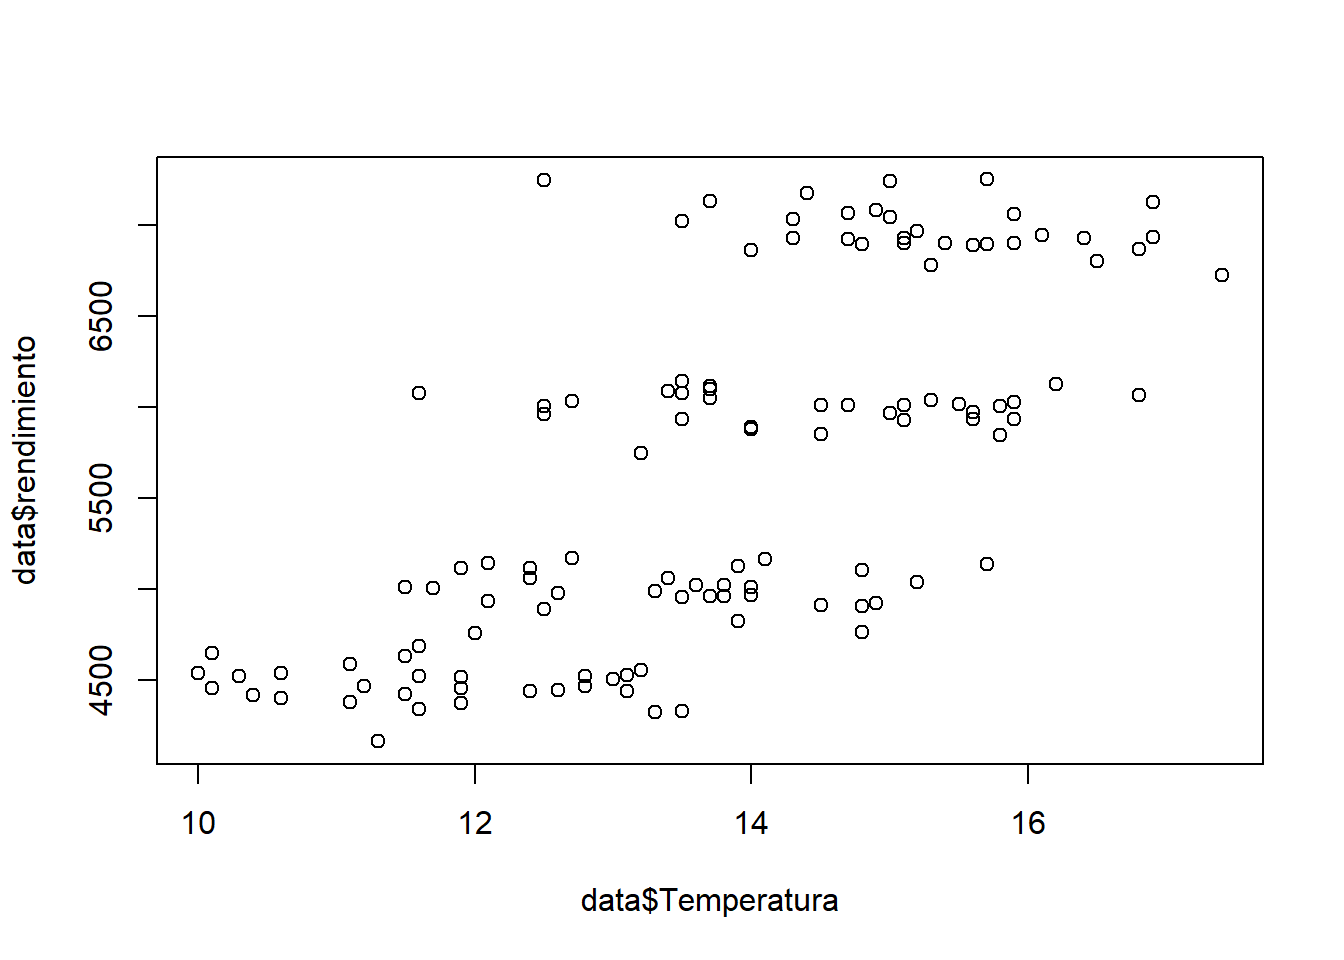
\includegraphics{04-lab_files/figure-latex/unnamed-chunk-1-1.pdf}

Felicitaciones, acaban de generar el primero de muchos gráficos que aprenderán en este curso. Sin embargo,
la tarea no está completa. Como podemos apreciar, el gráfico que nos entregó R es bastante ``rústico''.
Siempre intenten presentar sus datos de una forma atractiva. Esto puede marcar la diferencia entre un buen
trabajo y un trabajo sobresaliente.

Afortunadamente, R nos permite ``enchular'' nuestros gráficos. Para ello debemos ingresar comandos
específicos para cada una de las características que queremos modificar:

\begin{Shaded}
\begin{Highlighting}[]
\KeywordTok{plot}\NormalTok{(data}\OperatorTok{$}\NormalTok{Temperatura,data}\OperatorTok{$}\NormalTok{rendimiento,}
\DataTypeTok{xlab =} \StringTok{"Temperatura ambiental (Celcius)"}\NormalTok{,}
\DataTypeTok{ylab =} \StringTok{"Rendimiento (Ton/hect)"}\NormalTok{,}
\DataTypeTok{xlim =} \KeywordTok{c}\NormalTok{(}\DecValTok{9}\NormalTok{,}\DecValTok{18}\NormalTok{),}
\DataTypeTok{ylim =} \KeywordTok{c}\NormalTok{(}\DecValTok{4000}\NormalTok{,}\DecValTok{8000}\NormalTok{),}
\DataTypeTok{main =} \StringTok{"Mi primer grafico en R"}\NormalTok{,}
\DataTypeTok{pch=}\DecValTok{20}\NormalTok{,}
\DataTypeTok{col=}\StringTok{"red"}\NormalTok{,}
\DataTypeTok{cex=}\DecValTok{2}\NormalTok{,}
\DataTypeTok{cex.lab=}\FloatTok{1.2}\NormalTok{,}
\DataTypeTok{cex.axis=}\FloatTok{1.1}\NormalTok{)}
\end{Highlighting}
\end{Shaded}

\includegraphics{04-lab_files/figure-latex/unnamed-chunk-2-1.pdf}

A simple vista, son múltiples los parámetros gráficos que hemos cambiado. A continuación, se detalla la
lista de los parámetros utilizados y sus definiciones:

\begin{itemize}
\item
  \texttt{xlab} = Permite modificar el nombre del eje x
\item
  \texttt{ylab} = Permite modificar el nombre del eje y
\item
  \texttt{xlim} = Establece los limites del eje x
\item
  \texttt{ylim} = Establece los limites del eje y
\item
  \texttt{main} = Permite agregar un título a nuestro gráfico
\item
  \texttt{pch} = Permite modificar la forma de los puntos en nuestro gráfico
\item
  \texttt{col} = Permite modificar el color
\item
  \texttt{cex} = Permite modificar el tamaño del texto
\end{itemize}

Para aprender sobre otros comandos que permiten modificar parámetros les sugerimos visitar el siguiente \href{https://www.statmethods.net/advgraphs/parameters.html}{link}.

Nunca olviden que aprender R implica un constante prueba y error, por lo cual ahora que tienen una lista de
parámetros, comiencen a probar que sucede cuando cambian los valores de cada uno de ellos. No tengan
miedo a equivocarse!

Hasta ahora hemos generados dos gráficos, sin embargo solo podemos ver uno a la vez. R proporciona los
comandos necesarios para ver más de un gráfico de forma simultánea. Con la función \texttt{par()}, podemos
incluir la opción \texttt{mfrow=c()} para crear una matriz de filas y columnas.

Utilicemos los dos scatterplot anteriores para generar una matriz gráfica que contenga dos gráficos
ordenados en una fila y con dos columnas:

\begin{Shaded}
\begin{Highlighting}[]
\KeywordTok{par}\NormalTok{(}\DataTypeTok{mfrow=}\KeywordTok{c}\NormalTok{(}\DecValTok{1}\NormalTok{,}\DecValTok{2}\NormalTok{))}

\KeywordTok{plot}\NormalTok{(data}\OperatorTok{$}\NormalTok{Temperatura,data}\OperatorTok{$}\NormalTok{rendimiento)}

\KeywordTok{plot}\NormalTok{(data}\OperatorTok{$}\NormalTok{Temperatura,data}\OperatorTok{$}\NormalTok{rendimiento,}
\DataTypeTok{xlab =} \StringTok{"Temperatura ambiental (Celcius)"}\NormalTok{,}
\DataTypeTok{ylab =} \StringTok{"Rendimiento (Ton/hect)"}\NormalTok{,}
\DataTypeTok{xlim =} \KeywordTok{c}\NormalTok{(}\DecValTok{9}\NormalTok{,}\DecValTok{18}\NormalTok{),}
\DataTypeTok{ylim =} \KeywordTok{c}\NormalTok{(}\DecValTok{4000}\NormalTok{,}\DecValTok{8000}\NormalTok{),}
\DataTypeTok{main =} \StringTok{"Mi primer grafico en R"}\NormalTok{,}
\DataTypeTok{pch=}\DecValTok{20}\NormalTok{,}
\DataTypeTok{col=}\StringTok{"red"}\NormalTok{,}
\DataTypeTok{cex=}\FloatTok{1.5}\NormalTok{,}
\DataTypeTok{cex.lab=}\FloatTok{1.0}\NormalTok{,}
\DataTypeTok{cex.axis=}\FloatTok{1.0}\NormalTok{)}
\end{Highlighting}
\end{Shaded}

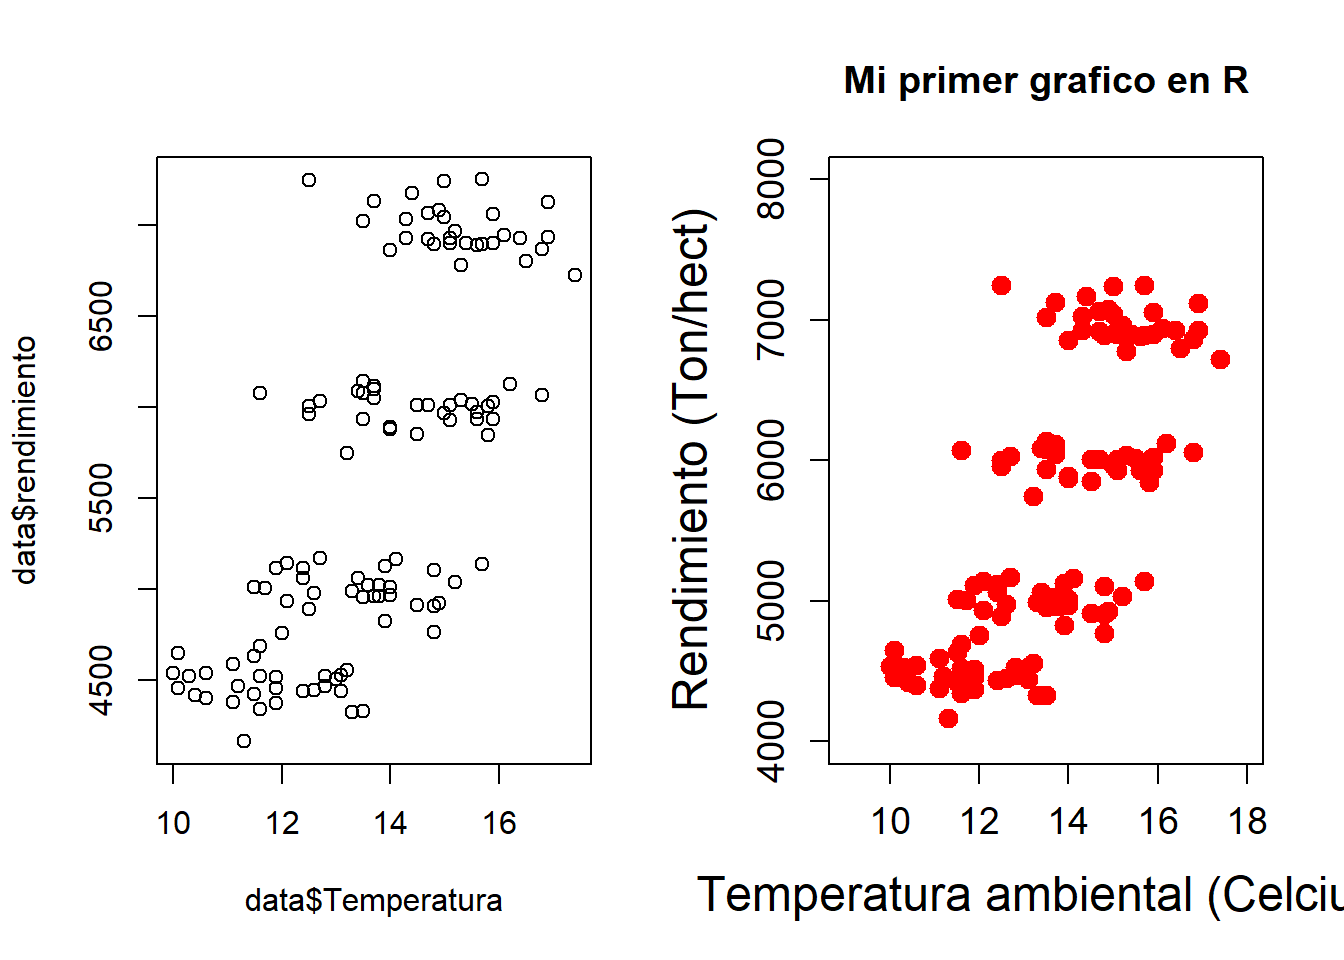
\includegraphics{04-lab_files/figure-latex/unnamed-chunk-3-1.pdf}

Fantástico! Tenemos ambos scatterplot graficados al mismo tiempo, uno al lado del otro. Ahora bien, en
caso de que quisiéramos que estén un scatterplot sobre el otro, ¿¿como lo harían??

\hypertarget{diagrama-de-cajas-o-boxplot}{%
\section{\texorpdfstring{Diagrama de cajas o \emph{Boxplot}}{Diagrama de cajas o Boxplot}}\label{diagrama-de-cajas-o-boxplot}}

Un diagrama de cajas es un gráfico que está basado en cuartiles y mediante el cual se visualiza la

distribución de un conjunto de datos. Está compuesto por un rectángulo (la «caja») y dos brazos (los
«bigotes»). Los diagramas de caja se pueden crear para variables individuales o para grupos de variables.

La función es \texttt{boxplot(x)}, donde \texttt{x} es nuestra variable a graficar:

Generemos un gráfico de cajas para la información contenida en la variable rendimiento:

\begin{Shaded}
\begin{Highlighting}[]
\KeywordTok{boxplot}\NormalTok{(data}\OperatorTok{$}\NormalTok{rendimiento)}
\end{Highlighting}
\end{Shaded}

\includegraphics{04-lab_files/figure-latex/unnamed-chunk-4-1.pdf}

Ahora, generemos el diagrama para la información contenida en la variable rendimiento según la región en la
cual se realizó el muestreo (grupo de variable):

\begin{Shaded}
\begin{Highlighting}[]
\KeywordTok{boxplot}\NormalTok{(data}\OperatorTok{$}\NormalTok{rendimiento }\OperatorTok{~}\StringTok{ }\NormalTok{data}\OperatorTok{$}\NormalTok{Region)}
\end{Highlighting}
\end{Shaded}

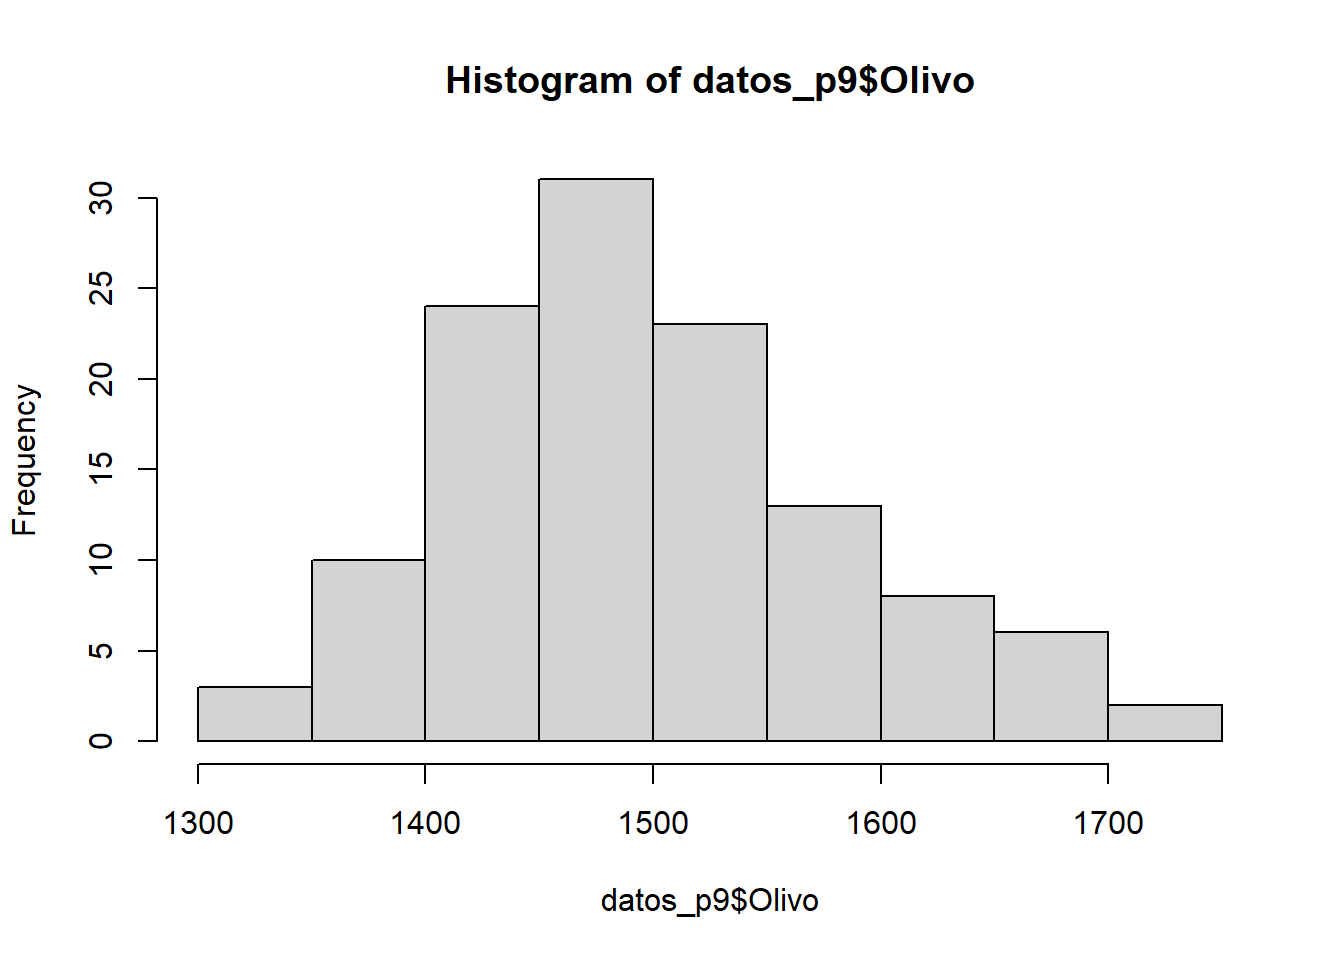
\includegraphics{04-lab_files/figure-latex/unnamed-chunk-5-1.pdf}

En caso de que quisiéramos enchular nuestro gráfico de cajas con dos variables, solamente debemos
modificar los parámetros gráficos:

\begin{Shaded}
\begin{Highlighting}[]
\KeywordTok{plot}\NormalTok{(data}\OperatorTok{$}\NormalTok{rendimiento }\OperatorTok{~}\StringTok{ }\NormalTok{data}\OperatorTok{$}\NormalTok{Region,}
\DataTypeTok{xlab =} \StringTok{"Region"}\NormalTok{,}
\DataTypeTok{ylab =} \StringTok{"Rendimiento (Ton/hect)"}\NormalTok{,}
\DataTypeTok{ylim =} \KeywordTok{c}\NormalTok{(}\DecValTok{4000}\NormalTok{,}\DecValTok{8000}\NormalTok{),}
\DataTypeTok{main =} \StringTok{"Diagrama de cajas"}\NormalTok{,}
\DataTypeTok{pch=}\DecValTok{18}\NormalTok{,}
\DataTypeTok{col=}\StringTok{"red"}\NormalTok{,}
\DataTypeTok{col.main=}\StringTok{"red"}\NormalTok{,}
\DataTypeTok{cex=}\DecValTok{2}\NormalTok{,}
\DataTypeTok{cex.main=}\FloatTok{1.5}\NormalTok{,}
\DataTypeTok{cex.lab=}\FloatTok{1.0}\NormalTok{,}
\DataTypeTok{cex.axis=}\FloatTok{1.0}\NormalTok{)}
\end{Highlighting}
\end{Shaded}

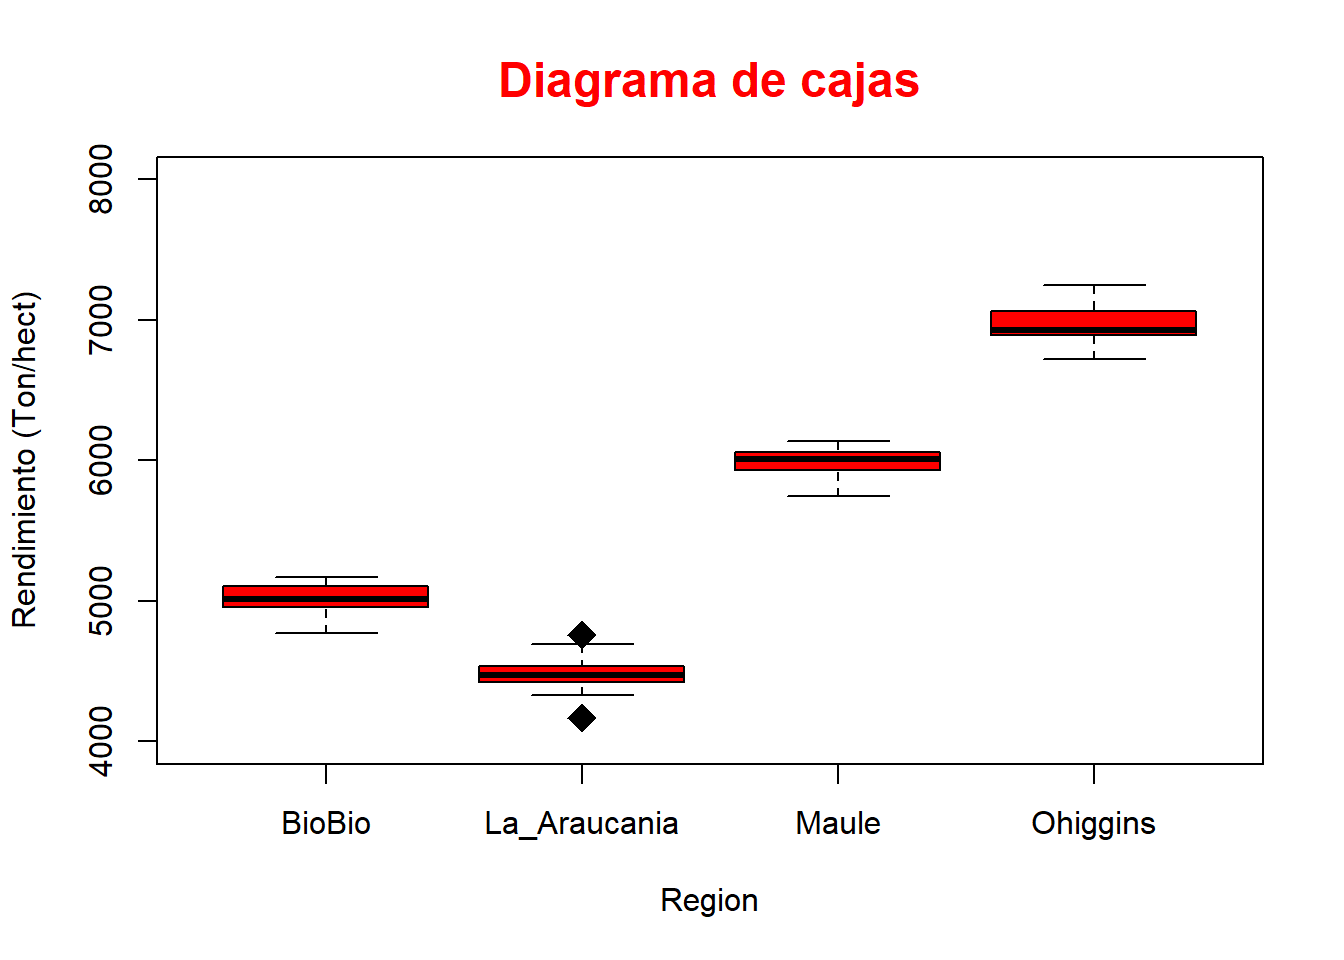
\includegraphics{04-lab_files/figure-latex/unnamed-chunk-6-1.pdf}

\hypertarget{histogramas}{%
\section{Histogramas}\label{histogramas}}

Un histograma es una representación visual de la distribución de un conjunto de datos. Como tal, la forma de
un histograma es su característica más obvia e informativa: nos permite ver fácilmente dónde está el medio
en su distribución de datos, qué tan cerca están los datos de este medio y dónde se encuentran posibles
valores atípicos.

El histograma consiste en un eje x, un eje y, además de varias barras de diferentes alturas. El eje y muestra
con qué frecuencia (número de veces que se repite una observación) se producen los valores en el eje,
mientras que las barras agrupan rangos de valores o categorías continuas en el eje x (intervalos). Esto explica
por qué los histogramas se llaman ``histograma de frecuencia''.

La función es \texttt{hist(x)}, donde \texttt{x} es nuestra variable a graficar.

Generemos un histograma de frecuencias para la información contenida en la variable rendimiento:

\begin{Shaded}
\begin{Highlighting}[]
\KeywordTok{hist}\NormalTok{(data}\OperatorTok{$}\NormalTok{rendimiento)}
\end{Highlighting}
\end{Shaded}

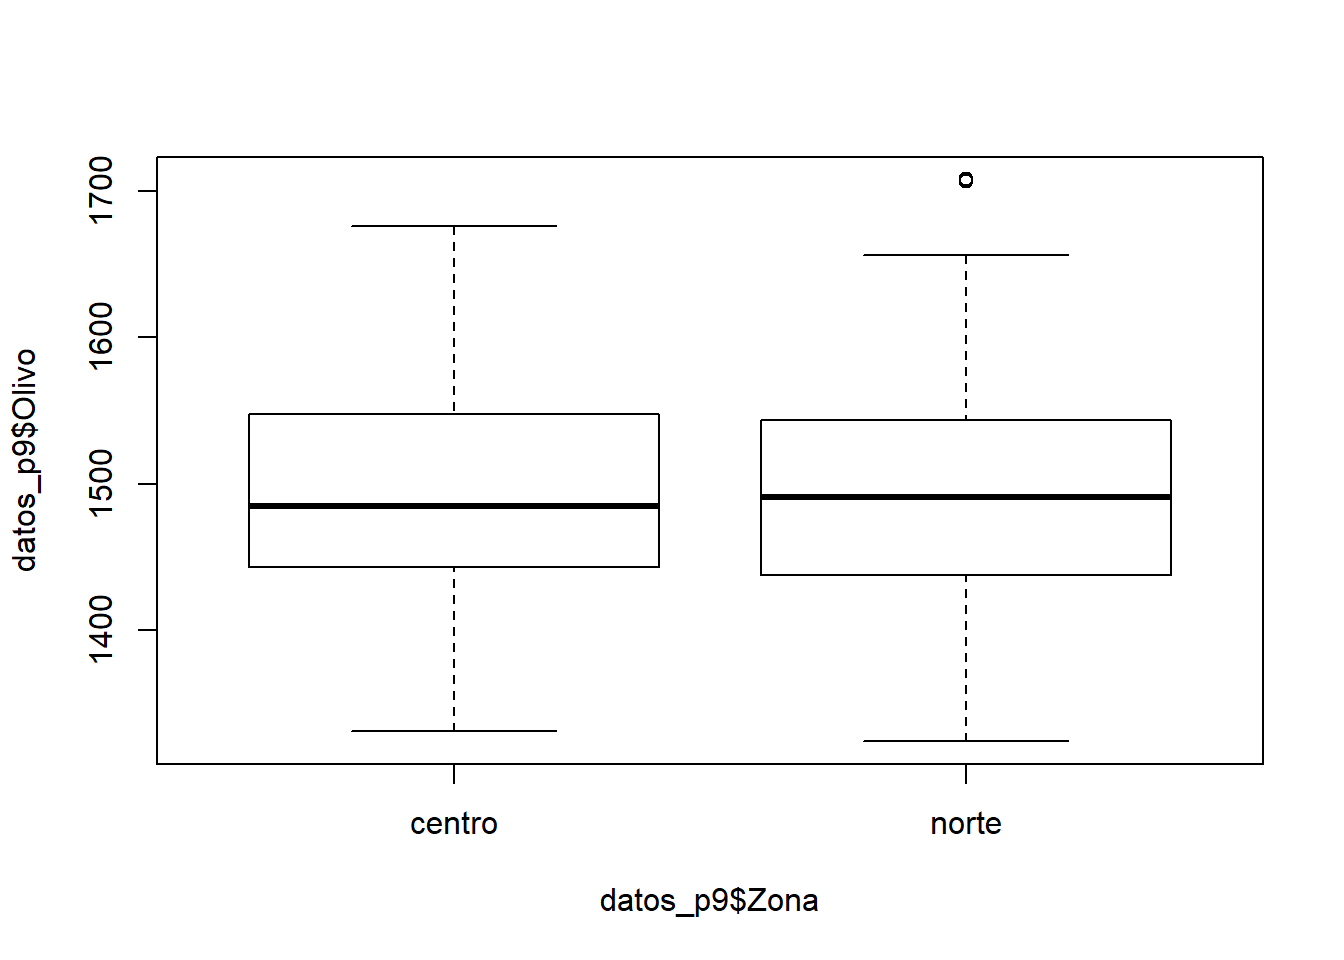
\includegraphics{04-lab_files/figure-latex/unnamed-chunk-7-1.pdf}

Al igual que los gráficos anteriores, R nos permite modificar parámetros gráficos de los histograma de
frecuencia. Por ejemplo, podemos especificar el número de intervalos en las cuales queremos que se agrupen
nuestros datos. Para ello utilizamos el comando \texttt{breaks=}.

Generemos un histograma de frecuencias para la información contenida en la variable rendimiento pero que
esté agrupada solamente en 4 intervalos:

\begin{Shaded}
\begin{Highlighting}[]
\KeywordTok{hist}\NormalTok{(data}\OperatorTok{$}\NormalTok{rendimiento,}\DataTypeTok{breaks=}\DecValTok{4}\NormalTok{)}
\end{Highlighting}
\end{Shaded}

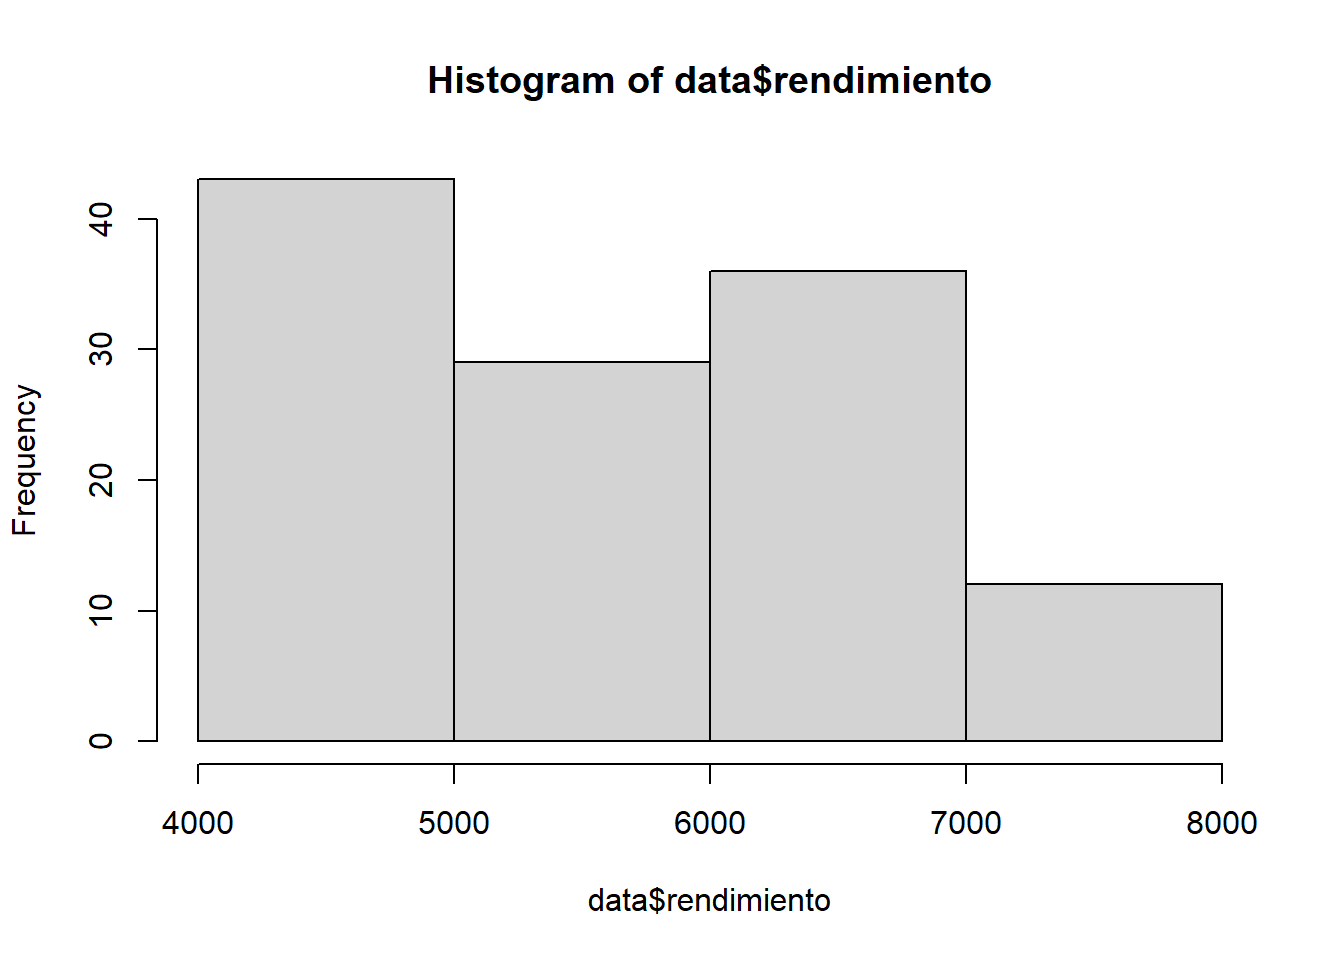
\includegraphics{04-lab_files/figure-latex/unnamed-chunk-8-1.pdf}

Intentemos algo más que nos servirá para los próximos laboratorios. En algunas ocasiones, estaremos más
interesados en la densidad (probabilidad relativa de un dato) que en la frecuencia de nuestros datos. En lugar
de contar el número de puntos de datos por intervalo, R puede dar las densidades de probabilidad usando la
opción \texttt{freq=\ FALSE}, lo cual nos permite normalizar el histograma de modo que el área total es igual a 1.
Ahora el eje y está etiquetado como densidad en lugar de frecuencia.

Modifiquemos nuestro histograma de frecuencia anterior por un histograma de densidad y grafiquemos uno
al lado del otro:

\begin{Shaded}
\begin{Highlighting}[]
\KeywordTok{par}\NormalTok{(}\DataTypeTok{mfrow=}\KeywordTok{c}\NormalTok{(}\DecValTok{1}\NormalTok{,}\DecValTok{2}\NormalTok{))}

\KeywordTok{hist}\NormalTok{(data}\OperatorTok{$}\NormalTok{rendimiento)}

\KeywordTok{hist}\NormalTok{(data}\OperatorTok{$}\NormalTok{rendimiento,}
\DataTypeTok{main=}\StringTok{"Histograma de densidad"}\NormalTok{,}
\DataTypeTok{xlab=}\StringTok{"Rendimiento (Ton/hect)"}\NormalTok{,}
\DataTypeTok{xlim=}\KeywordTok{c}\NormalTok{(}\DecValTok{3500}\NormalTok{,}\DecValTok{8500}\NormalTok{),}
\DataTypeTok{col=}\StringTok{"red"}\NormalTok{,}
\DataTypeTok{freq=}\OtherTok{FALSE}\NormalTok{,}
\DataTypeTok{cex.main=}\FloatTok{1.2}\NormalTok{,}
\DataTypeTok{cex.lab=}\FloatTok{1.0}\NormalTok{,}
\DataTypeTok{cex.axis=}\FloatTok{1.0}\NormalTok{,}
\DataTypeTok{Freq=}\OtherTok{FALSE}\NormalTok{)}
\end{Highlighting}
\end{Shaded}

\begin{verbatim}
## Warning in plot.window(xlim, ylim, "", ...): "Freq" is not a graphical
## parameter
\end{verbatim}

\begin{verbatim}
## Warning in title(main = main, sub = sub, xlab = xlab, ylab = ylab, ...):
## "Freq" is not a graphical parameter
\end{verbatim}

\begin{verbatim}
## Warning in axis(1, ...): "Freq" is not a graphical parameter
\end{verbatim}

\begin{verbatim}
## Warning in axis(2, ...): "Freq" is not a graphical parameter
\end{verbatim}

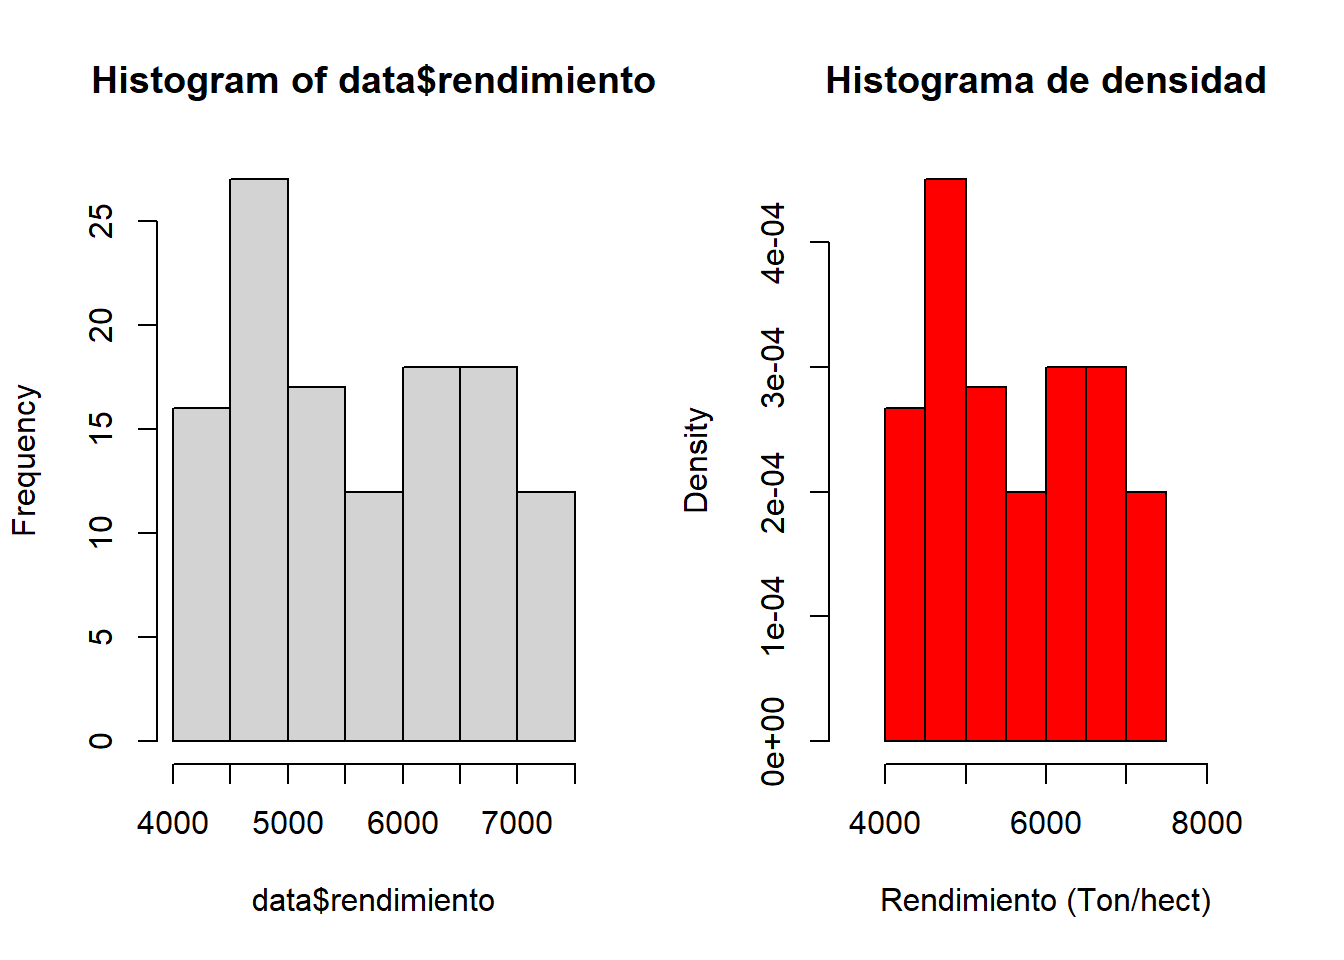
\includegraphics{04-lab_files/figure-latex/unnamed-chunk-9-1.pdf}

\hypertarget{ejercicios-para-la-casa}{%
\section{Ejercicios para la casa}\label{ejercicios-para-la-casa}}

\begin{enumerate}
\def\labelenumi{\arabic{enumi}.}
\item
  Generar un gráfico que permita visualizar la relación entre las variables Temperatura y rendimiento.
  El gráfico debe contener solamente los datos obtenidos de las regiones del Maule y Araucanía.
\item
  Generar un histograma de frecuencia con los rendimientos superiores a 5000 Toneladas/hectárea.
\item
  Generar un gráfico de cajas para la variedad 1 que muestre solamente los rendimientos superiores a
  5000 Toneladas/hectárea.
\end{enumerate}

\hypertarget{estaduxedstica-descriptiva-medidas-de-tendencia-central-y-dispersiuxf3n}{%
\chapter{Estadística descriptiva: Medidas de tendencia central y dispersión}\label{estaduxedstica-descriptiva-medidas-de-tendencia-central-y-dispersiuxf3n}}

En el laboratorio anterior aprendimos a graficar la información contenida en nuestra base de datos. El paso siguiente es resumir la información contenida en nuestra base de datos mediante la estimación de medidas de tendencia central y dispersión.

\hypertarget{medidas-de-tendencia-central}{%
\section{Medidas de tendencia central}\label{medidas-de-tendencia-central}}

Las medidas de tendencia central son medidas estadísticas que permiten resumir en un solo valor a un conjunto de valores. Representan un centro en torno al cual se encuentra ubicado el conjunto de los datos.

Las medidas de tendencia central más utilizadas son: media, mediana y moda.

\textbf{Funciones:}

\begin{itemize}
\item
  \texttt{sum(x)}: Suma de los elementos en \texttt{x}
\item
  \texttt{mean(x)}: Promedio de los elementos en \texttt{x}
\item
  \texttt{median(x)}: Mediana de los elementos en \texttt{x}
\item
  \texttt{length(x)}: Número de elementos en \texttt{x}
\end{itemize}

Calculemos el promedio y la mediana de la temperatura ambiental en todas las muestras incluidas en nuestra base de datos:

\begin{Shaded}
\begin{Highlighting}[]
\KeywordTok{mean}\NormalTok{(data}\OperatorTok{$}\NormalTok{Temperatura)}
\end{Highlighting}
\end{Shaded}

\begin{verbatim}
## [1] 13.74167
\end{verbatim}

\begin{Shaded}
\begin{Highlighting}[]
\KeywordTok{median}\NormalTok{(data}\OperatorTok{$}\NormalTok{Temperatura)}
\end{Highlighting}
\end{Shaded}

\begin{verbatim}
## [1] 13.75
\end{verbatim}

Estas estimaciones las hemos realizado sobre todas las observaciones contenidas en nuestra variable. Sin embargo, en algunas ocasiones, estaremos interesados en un subconjunto de las observaciones que cumplan con alguna condición de nuestro interés. Por ejemplo, podemos estar interesados en el promedio de la temperatura ambiental en aquellas muestras que provienen solamente de la región del Maule. Para seleccionar aquellas muestras que cumplen con esta restricción podemos generar un subconjunto o subset:

\texttt{"Nombre\ del\ objeto"\ \textless{}-\ "base\ de\ datos"\$\ "columna\ de\ interés"\ ==\ "restricción"}

\begin{Shaded}
\begin{Highlighting}[]
\NormalTok{subset_data <-}\StringTok{ }\NormalTok{data}\OperatorTok{$}\NormalTok{Region }\OperatorTok{==}\StringTok{ "Maule"}
\NormalTok{subset_data}
\end{Highlighting}
\end{Shaded}

\begin{verbatim}
##   [1] FALSE FALSE FALSE FALSE FALSE FALSE FALSE FALSE FALSE FALSE FALSE
##  [12] FALSE FALSE FALSE FALSE FALSE FALSE FALSE FALSE FALSE FALSE FALSE
##  [23] FALSE FALSE FALSE FALSE FALSE FALSE FALSE FALSE  TRUE  TRUE  TRUE
##  [34]  TRUE  TRUE  TRUE  TRUE  TRUE  TRUE  TRUE  TRUE  TRUE  TRUE  TRUE
##  [45]  TRUE  TRUE  TRUE  TRUE  TRUE  TRUE  TRUE  TRUE  TRUE  TRUE  TRUE
##  [56]  TRUE  TRUE  TRUE  TRUE  TRUE FALSE FALSE FALSE FALSE FALSE FALSE
##  [67] FALSE FALSE FALSE FALSE FALSE FALSE FALSE FALSE FALSE FALSE FALSE
##  [78] FALSE FALSE FALSE FALSE FALSE FALSE FALSE FALSE FALSE FALSE FALSE
##  [89] FALSE FALSE FALSE FALSE FALSE FALSE FALSE FALSE FALSE FALSE FALSE
## [100] FALSE FALSE FALSE FALSE FALSE FALSE FALSE FALSE FALSE FALSE FALSE
## [111] FALSE FALSE FALSE FALSE FALSE FALSE FALSE FALSE FALSE FALSE
\end{verbatim}

Al revisar el contenido de nuestro objeto llamado \texttt{subset\_data}, R nos dice cuál o cuáles de las observaciones cumplen (TRUE) o no cumplen (FALSE) con nuestro requerimiento. Ahora, podemos calcular el promedio de la temperatura ambiental promedio en aquellas muestras que provienen solamente de la región del Maule:

\begin{Shaded}
\begin{Highlighting}[]
\KeywordTok{mean}\NormalTok{(data}\OperatorTok{$}\NormalTok{Temperatura[subset_data])}
\end{Highlighting}
\end{Shaded}

\begin{verbatim}
## [1] 14.42667
\end{verbatim}

\hypertarget{operadores-luxf3gicos}{%
\subsection{Operadores lógicos}\label{operadores-luxf3gicos}}

\begin{itemize}
\item
  \texttt{==} Igual a\ldots{}
\item
  \texttt{¡=} No es igual a\ldots{}
\item
  \texttt{\textgreater{}} Mayor que\ldots{}
\item
  \texttt{\textless{}} Menor que\ldots{}
\item
  \texttt{\textgreater{}=} Mayor o igual que\ldots{}
\item
  \texttt{\textless{}=} Menor o igual que\ldots{}
\item
  \texttt{\textbar{}} ``o'' (al menos una de las condiciones debe ser cierta)
\item
  \texttt{\&} ``y'' (ambas condiciones deben ser ciertas)
\end{itemize}

Para estimar el número de observaciones que cumplen con nuestra condición podemos utilizar la función \texttt{length()}:

\begin{Shaded}
\begin{Highlighting}[]
\KeywordTok{length}\NormalTok{(data}\OperatorTok{$}\NormalTok{Temperatura[subset_data])}
\end{Highlighting}
\end{Shaded}

\begin{verbatim}
## [1] 30
\end{verbatim}

Regresemos a nuestra base de datos. Pasos atrás calculamos el promedio de la temperatura ambiental en todas las muestras incluidas en nuestra base de datos. Eso es un gran paso para describir la variable temperatura ambiental. Sin embargo, la base de datos contiene mucha información adicional que nos permitirá describir de mejor forma la temperatura ambiental registrada en nuestro estudio. Por ejemplo, podríamos preguntarnos si la temperatura ambiental difiere según la región en la que fue medida. Para ello, debemos conocer el promedio de la variable Temperatura para las cuatro diferentes regiones contenidas en la variable Region. Una opción es generar cuatro diferentes ``subset'':

\begin{Shaded}
\begin{Highlighting}[]
\NormalTok{subset1<-data}\OperatorTok{$}\NormalTok{Region }\OperatorTok{==}\StringTok{ "Ohiggins"}
\KeywordTok{mean}\NormalTok{(data}\OperatorTok{$}\NormalTok{Temperatura[subset1])}
\end{Highlighting}
\end{Shaded}

\begin{verbatim}
## [1] 15.25667
\end{verbatim}

\begin{Shaded}
\begin{Highlighting}[]
\NormalTok{subset2<-data}\OperatorTok{$}\NormalTok{Region }\OperatorTok{==}\StringTok{ "Maule"}
\KeywordTok{mean}\NormalTok{(data}\OperatorTok{$}\NormalTok{Temperatura[subset2])}
\end{Highlighting}
\end{Shaded}

\begin{verbatim}
## [1] 14.42667
\end{verbatim}

\begin{Shaded}
\begin{Highlighting}[]
\NormalTok{subset3<-data}\OperatorTok{$}\NormalTok{Region }\OperatorTok{==}\StringTok{ "BioBio"}
\KeywordTok{mean}\NormalTok{(data}\OperatorTok{$}\NormalTok{Temperatura[subset3])}
\end{Highlighting}
\end{Shaded}

\begin{verbatim}
## [1] 13.54667
\end{verbatim}

\begin{Shaded}
\begin{Highlighting}[]
\NormalTok{subset4<-data}\OperatorTok{$}\NormalTok{Region }\OperatorTok{==}\StringTok{ "La_Araucania"}
\KeywordTok{mean}\NormalTok{(data}\OperatorTok{$}\NormalTok{Temperatura[subset4])}
\end{Highlighting}
\end{Shaded}

\begin{verbatim}
## [1] 11.73667
\end{verbatim}

Afortunadamente, R nos ofrece alternativas mucho más eficientes y elegantes para realizar la misma tarea. Por ejemplo, `tapply()``aplica una función (en este caso mean()) a cada grupo de observaciones de una variable definidos por los niveles de una segunda variable:

\begin{Shaded}
\begin{Highlighting}[]
\KeywordTok{tapply}\NormalTok{(data}\OperatorTok{$}\NormalTok{Temperatura,data}\OperatorTok{$}\NormalTok{Region,mean)}
\end{Highlighting}
\end{Shaded}

\begin{verbatim}
##       BioBio La_Araucania        Maule     Ohiggins 
##     13.54667     11.73667     14.42667     15.25667
\end{verbatim}

Incluso, R nos permite guardar nuestros cálculos en forma de objeto:

\begin{Shaded}
\begin{Highlighting}[]
\NormalTok{Temperatura_regional<-}\KeywordTok{tapply}\NormalTok{(data}\OperatorTok{$}\NormalTok{Temperatura,data}\OperatorTok{$}\NormalTok{Region,mean)}
\NormalTok{Temperatura_regional}
\end{Highlighting}
\end{Shaded}

\begin{verbatim}
##       BioBio La_Araucania        Maule     Ohiggins 
##     13.54667     11.73667     14.42667     15.25667
\end{verbatim}

\hypertarget{medidas-de-dispersiuxf3n}{%
\section{Medidas de dispersión}\label{medidas-de-dispersiuxf3n}}

A diferencia de las medidas de tendencia central, las medidas de dispersión sirven como indicador de la variabilidad de los datos de la variable. Dicho en otros términos, las medidas de dispersión pretenden evaluar en qué medida los datos difieren entre sí. Las medidas de tendencia central más utilizadas son: desviación estándar, varianza y el coeficiente de variación.

\textbf{Funciones:}

\begin{itemize}
\item
  \texttt{var(x)} Varianza de los elementos en x
\item
  \texttt{sd(x)} Desviación estándar de los elementos en x
\item
  \texttt{range(x)} Rango de los elementos en x
\item
  \texttt{min(x)} Mínimo valor observado entre los elementos en x
\item
  \texttt{max(x)} Máximo valor observado entre los elementos en x
\end{itemize}

Calculemos la desviación estándar y la varianza de la temperatura ambiental en todas las muestras incluidas en nuestra base de datos:

\begin{Shaded}
\begin{Highlighting}[]
\KeywordTok{sd}\NormalTok{(data}\OperatorTok{$}\NormalTok{Temperatura)}
\end{Highlighting}
\end{Shaded}

\begin{verbatim}
## [1] 1.736972
\end{verbatim}

\begin{Shaded}
\begin{Highlighting}[]
\KeywordTok{var}\NormalTok{(data}\OperatorTok{$}\NormalTok{Temperatura)}
\end{Highlighting}
\end{Shaded}

\begin{verbatim}
## [1] 3.017073
\end{verbatim}

Intentemos calcular manualmente la desviación estándar a partir de la varianza:

\begin{Shaded}
\begin{Highlighting}[]
\NormalTok{desvest <-}\StringTok{ }\KeywordTok{sqrt}\NormalTok{(}\KeywordTok{var}\NormalTok{(data}\OperatorTok{$}\NormalTok{Temperatura))}
\end{Highlighting}
\end{Shaded}

Ahora, evaluemos si la desviación estándar de la temperatura ambiental difiere según la región en la que fue medida:

\begin{Shaded}
\begin{Highlighting}[]
\NormalTok{desvest_temperatura <-}\StringTok{ }\KeywordTok{tapply}\NormalTok{(data}\OperatorTok{$}\NormalTok{Temperatura,data}\OperatorTok{$}\NormalTok{Region,sd)}
\NormalTok{desvest_temperatura}
\end{Highlighting}
\end{Shaded}

\begin{verbatim}
##       BioBio La_Araucania        Maule     Ohiggins 
##     1.136156     1.064630     1.291333     1.109422
\end{verbatim}

El Coeficiente de variación (C.V.) es un índice adimensional de variabilidad especialmente útil para comparar variabilidades de características de diferente naturaleza o de la misma naturaleza en diferentes grupos. El C.V. se obtiene al dividir la desviación estándar por la media aritmética, y multiplicado este cuociente por 100. A mayor valor del C.V. mayor heterogeneidad (variabilidad) de los valores de la variable; y a menor C.V. mayor homogeneidad en los valores de la variable.

En caso de que estuviésemos interesados en comparar la variabilidad existente en las variables temperatura ambiental y superficie cultivada (dos variables de naturaleza diferente), el coeficiente de variación es de gran utilidad:

\begin{Shaded}
\begin{Highlighting}[]
\NormalTok{cv_temperatura<-}\StringTok{ }\NormalTok{(}\KeywordTok{sd}\NormalTok{(data}\OperatorTok{$}\NormalTok{Temperatura)}\OperatorTok{/}\KeywordTok{mean}\NormalTok{(data}\OperatorTok{$}\NormalTok{Temperatura))}\OperatorTok{*}\DecValTok{100}
\NormalTok{cv_temperatura}
\end{Highlighting}
\end{Shaded}

\begin{verbatim}
## [1] 12.64019
\end{verbatim}

\begin{Shaded}
\begin{Highlighting}[]
\NormalTok{cv_superficie<-}\StringTok{ }\NormalTok{(}\KeywordTok{sd}\NormalTok{(data}\OperatorTok{$}\NormalTok{Hectareas)}\OperatorTok{/}\KeywordTok{mean}\NormalTok{(data}\OperatorTok{$}\NormalTok{Hectareas))}\OperatorTok{*}\DecValTok{100}
\NormalTok{cv_superficie}
\end{Highlighting}
\end{Shaded}

\begin{verbatim}
## [1] 46.64448
\end{verbatim}

De acuerdo a nuestros resultados, la variable superficie cultivada (\texttt{Hectareas}) presenta mayor variabilidad (casi 3 veces) que la variable temperatura ambiental (\texttt{Temperatura}).

\hypertarget{tabla-resumen}{%
\section{Tabla Resumen}\label{tabla-resumen}}

Las medidas de tendencia central y dispersión las podemos presentar por medio de una tabla resumen. Una tabla representa un medio para organizar datos en filas y columnas. Para crear nuestra tabla resumen, podemos generar un objeto utilizando el comando \texttt{cbind()}, el cual nos permite unir diferentes columnas. Por otro lado el comando \texttt{rbind()} nos permite unir diferentes filas.

Ahora, generaremos una tabla que resuma la información contenida en la variable temperatura ambiental. Esta tabla nos especificará como el promedio, mediana, desviación estándar y coeficiente de variación difiere entre las diferentes regiones. Para ello utilizaremos la función \texttt{tapply()}.

Lo primero que haremos será generar 4 objetos que contengan las medidas que nos interesan:

\begin{Shaded}
\begin{Highlighting}[]
\NormalTok{promedio_temp<-}\KeywordTok{tapply}\NormalTok{(data}\OperatorTok{$}\NormalTok{Temperatura,data}\OperatorTok{$}\NormalTok{Region, mean)}
\NormalTok{promedio_temp}
\end{Highlighting}
\end{Shaded}

\begin{verbatim}
##       BioBio La_Araucania        Maule     Ohiggins 
##     13.54667     11.73667     14.42667     15.25667
\end{verbatim}

\begin{Shaded}
\begin{Highlighting}[]
\NormalTok{mediana_temp<-}\KeywordTok{tapply}\NormalTok{(data}\OperatorTok{$}\NormalTok{Temperatura,data}\OperatorTok{$}\NormalTok{Region, median)}
\NormalTok{mediana_temp}
\end{Highlighting}
\end{Shaded}

\begin{verbatim}
##       BioBio La_Araucania        Maule     Ohiggins 
##        13.75        11.60        14.50        15.15
\end{verbatim}

\begin{Shaded}
\begin{Highlighting}[]
\NormalTok{desvest_temp<-}\KeywordTok{tapply}\NormalTok{(data}\OperatorTok{$}\NormalTok{Temperatura,data}\OperatorTok{$}\NormalTok{Region, sd)}
\NormalTok{desvest_temp}
\end{Highlighting}
\end{Shaded}

\begin{verbatim}
##       BioBio La_Araucania        Maule     Ohiggins 
##     1.136156     1.064630     1.291333     1.109422
\end{verbatim}

\begin{Shaded}
\begin{Highlighting}[]
\NormalTok{coefvar_temp<-}\StringTok{ }\NormalTok{(desvest_temperatura}\OperatorTok{/}\NormalTok{promedio_temp)}\OperatorTok{*}\DecValTok{100}
\NormalTok{coefvar_temp}
\end{Highlighting}
\end{Shaded}

\begin{verbatim}
##       BioBio La_Araucania        Maule     Ohiggins 
##     8.386979     9.070973     8.951012     7.271716
\end{verbatim}

Podemos genera la tabla con el comando \texttt{cbind()}. Le especificaremos a R que cada uno de nuestros objetos será una columna en nuestra tabla:

\begin{Shaded}
\begin{Highlighting}[]
\NormalTok{tabla_resumen<-}\KeywordTok{cbind}\NormalTok{(promedio_temp,mediana_temp, desvest_temp, coefvar_temp)}
\NormalTok{tabla_resumen}
\end{Highlighting}
\end{Shaded}

\begin{verbatim}
##              promedio_temp mediana_temp desvest_temp coefvar_temp
## BioBio            13.54667        13.75     1.136156     8.386979
## La_Araucania      11.73667        11.60     1.064630     9.070973
## Maule             14.42667        14.50     1.291333     8.951012
## Ohiggins          15.25667        15.15     1.109422     7.271716
\end{verbatim}

Aunque una tabla resumen encierra toda la información disponible, siempre es recomendable realizar un análisis visual de los datos. Para ello debemos\ldots graficar!

\hypertarget{gruxe1fico-de-barras}{%
\section{Gráfico de Barras}\label{gruxe1fico-de-barras}}

Un gráfico de barras (barplot) es uno de los gráficos más comunes. Nos muestra la relación entre una variable numérica (generalmente en el eje \texttt{y}) y una variable categórica (generalmente en el eje \texttt{x}). A continuación, generaremos un gráfico de barras para evaluar si la temperatura ambiental difiere según la región en la que fue medida.

Lo primero que haremos será generar (otra vez!) 2 objetos que contengan el promedio y la desviación estándar de la temperatura ambiental medida en cada una de las regiones.

\begin{Shaded}
\begin{Highlighting}[]
\NormalTok{promedio_temp<-}\KeywordTok{tapply}\NormalTok{(data}\OperatorTok{$}\NormalTok{Temperatura,data}\OperatorTok{$}\NormalTok{Region, mean)}
\NormalTok{promedio_temp}
\end{Highlighting}
\end{Shaded}

\begin{verbatim}
##       BioBio La_Araucania        Maule     Ohiggins 
##     13.54667     11.73667     14.42667     15.25667
\end{verbatim}

\begin{Shaded}
\begin{Highlighting}[]
\NormalTok{desvest_temp<-}\KeywordTok{tapply}\NormalTok{(data}\OperatorTok{$}\NormalTok{Temperatura,data}\OperatorTok{$}\NormalTok{Region, sd)}
\NormalTok{desvest_temp}
\end{Highlighting}
\end{Shaded}

\begin{verbatim}
##       BioBio La_Araucania        Maule     Ohiggins 
##     1.136156     1.064630     1.291333     1.109422
\end{verbatim}

Ahora, utilizaremos el primero de los objetos creados para graficar el promedio de la temperatura según la región en la que fue medida. Pare ello generaremos un objeto que contenga los comandos necesarios para generar nuestro gráfico de barras:

\begin{Shaded}
\begin{Highlighting}[]
\NormalTok{GRAFICO<-}\StringTok{ }\KeywordTok{barplot}\NormalTok{(promedio_temp, }\DataTypeTok{ylim=}\KeywordTok{c}\NormalTok{(}\DecValTok{0}\NormalTok{,}\DecValTok{20}\NormalTok{), }\DataTypeTok{xlab=}\StringTok{"Region"}\NormalTok{, }\DataTypeTok{ylab=}\StringTok{"Temperatura ambiental"}\NormalTok{,}\DataTypeTok{col=}\KeywordTok{c}\NormalTok{(}\StringTok{"indianred"}\NormalTok{,}\StringTok{"red3"}\NormalTok{,}\StringTok{"red4"}\NormalTok{,}\StringTok{"orangered"}\NormalTok{), }\DataTypeTok{main=} \StringTok{"promedio y desviacion estandar"}\NormalTok{)}
\end{Highlighting}
\end{Shaded}

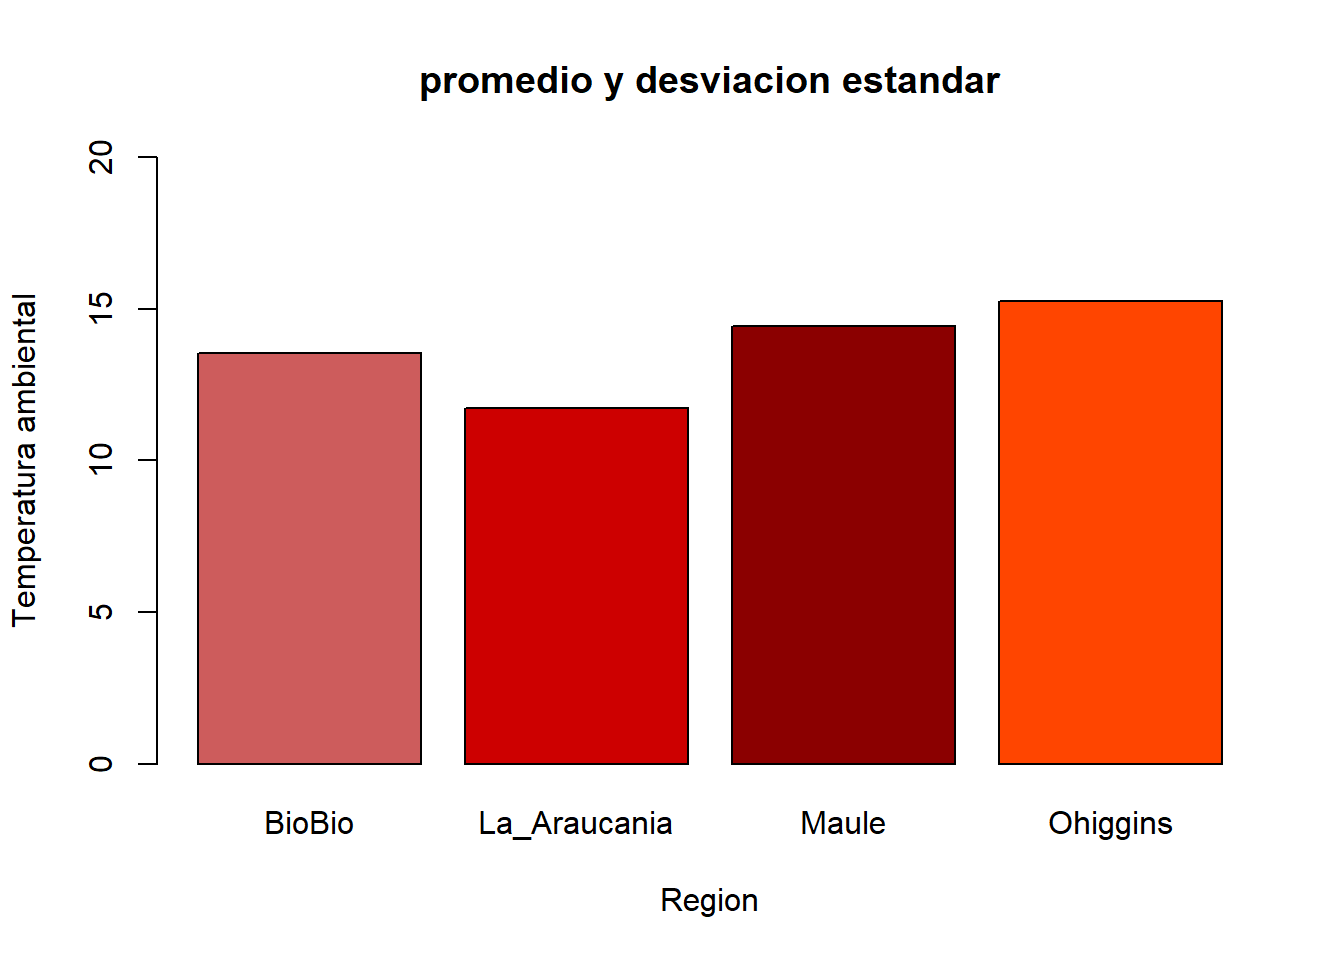
\includegraphics{05-lab_files/figure-latex/unnamed-chunk-26-1.pdf}

Solo nos falta agregar las respectivas desviaciones estándar asociadas a cada promedio. Pare ello utilizaremos el comando arrows y así agregar las líneas con las desviaciones estándar al objeto que contiene nuestro gráfico:

\begin{Shaded}
\begin{Highlighting}[]
\NormalTok{GRAFICO<-}\StringTok{ }\KeywordTok{barplot}\NormalTok{(promedio_temp, }\DataTypeTok{ylim=}\KeywordTok{c}\NormalTok{(}\DecValTok{0}\NormalTok{,}\DecValTok{20}\NormalTok{), }\DataTypeTok{xlab=}\StringTok{"Region"}\NormalTok{, }\DataTypeTok{ylab=}\StringTok{"Temperatura ambiental"}\NormalTok{,}\DataTypeTok{col=}\KeywordTok{c}\NormalTok{(}\StringTok{"indianred"}\NormalTok{,}\StringTok{"red3"}\NormalTok{,}\StringTok{"red4"}\NormalTok{,}\StringTok{"orangered"}\NormalTok{), }\DataTypeTok{main=} \StringTok{"promedio y desviacion estandar"}\NormalTok{)}
\KeywordTok{arrows}\NormalTok{(GRAFICO, promedio_temp }\OperatorTok{+}\StringTok{ }\NormalTok{desvest_temp, GRAFICO, promedio_temp }\OperatorTok{-}\StringTok{ }\NormalTok{desvest_temp,}
       \DataTypeTok{angle =} \DecValTok{90}\NormalTok{, }\DataTypeTok{code =} \DecValTok{1}\NormalTok{, }\DataTypeTok{length =} \FloatTok{0.1}\NormalTok{, }\DataTypeTok{col =} \KeywordTok{c}\NormalTok{(}\StringTok{"indianred"}\NormalTok{,}\StringTok{"red3"}\NormalTok{,}\StringTok{"red4"}\NormalTok{,}\StringTok{"orangered"}\NormalTok{))}
\end{Highlighting}
\end{Shaded}

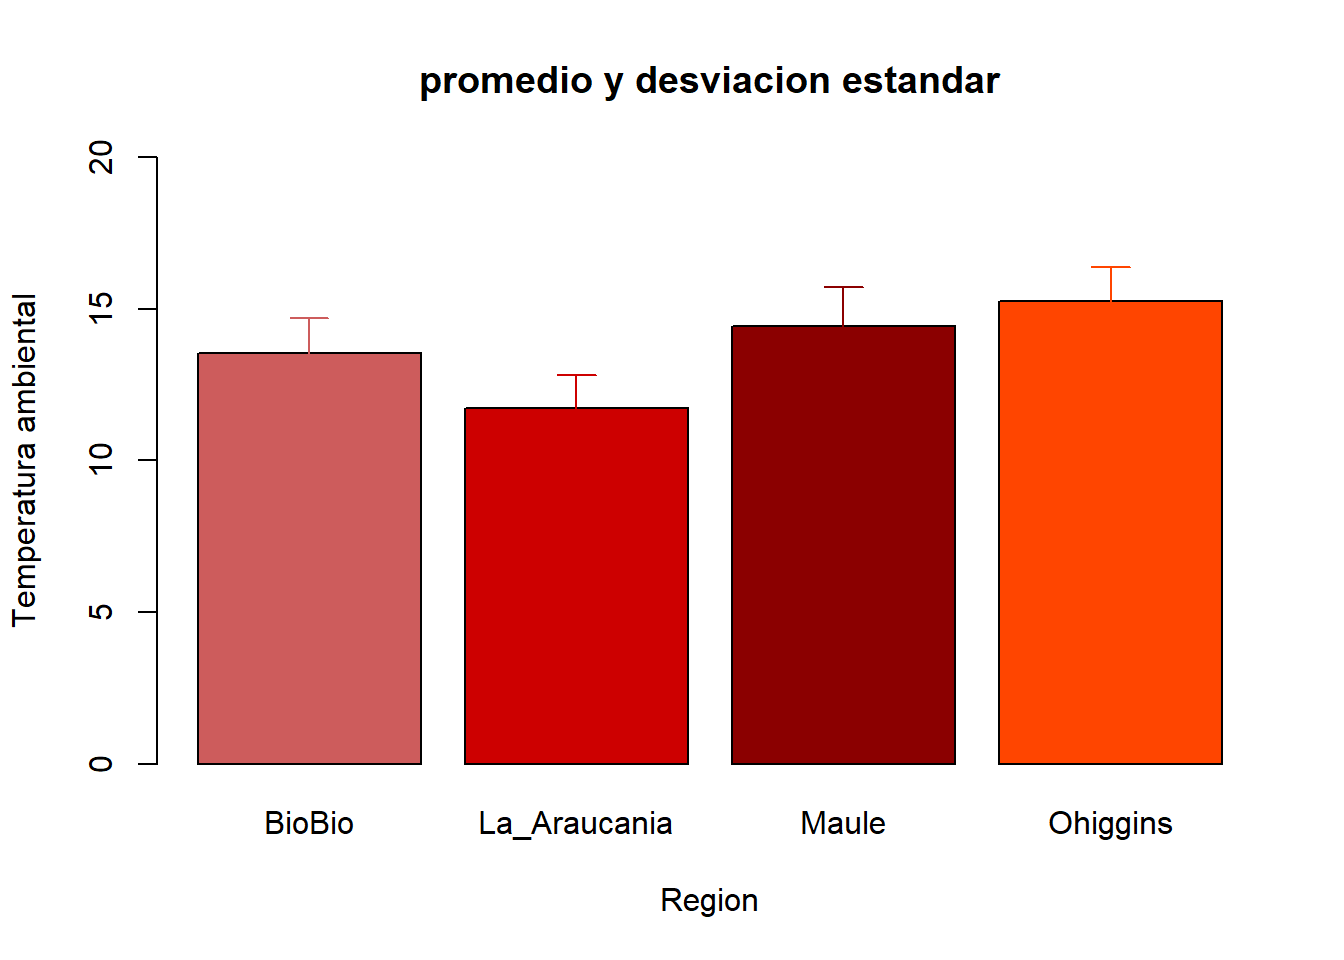
\includegraphics{05-lab_files/figure-latex/unnamed-chunk-27-1.pdf}

\hypertarget{estaduxedstica-inferencial-pruebas-estaduxedsticas}{%
\chapter{Estadística inferencial: Pruebas estadísticas}\label{estaduxedstica-inferencial-pruebas-estaduxedsticas}}

La Estadística inferencial es la rama de la Estadística que comprende los métodos empleados para deducir propiedades (hacer inferencias) de una población, a partir de una pequeña parte de la misma (muestra). También permite comparar muestras de diferentes poblaciones. Generalmente comprende las pruebas de estimación (puntual o por intervalos de confianza), y las pruebas de hipótesis.

En estadística inferencial existen dos grandes familias de pruebas estadísticas, las pruebas paramétricas y las no paramétricas.

\hypertarget{pruebas-paramuxe9tricas.}{%
\section{Pruebas paramétricas.}\label{pruebas-paramuxe9tricas.}}

Asumen que las muestras provienen de una población con una distribución conocida (generalmente distribución normal).

Para utilizar estas pruebas estadísticas, se deben cumplir algunas condiciones o supuestos:

\textbf{a. Normalidad}

Las pruebas paramétricas suponen que los datos se extraen de poblaciones que siguen una distribución normal. Es decir, los datos se distribuyen normalmente una vez que se tienen en cuenta los efectos de las variables en el modelo. En la práctica, esto significa que los residuos del análisis deberían distribuirse normalmente.

\textbf{b. Homogeneidad (homocedasticdad) de varianzas}

Las pruebas paramétricas consideran que la varianza es constante (no varía) en los diferentes grupos (niveles) de una variable (factor). Homoscedasticidad significa ``tener la misma dispersión''. Lo contrario es la heterocedasticidad (``dispersión diferente''). Datos atípicos modifican la varianza.

\textbf{c.~Independencia}

Los datos deben ser independientes unos de otros.

\hypertarget{pruebas-no-paramuxe9tricas}{%
\section{Pruebas no-paramétricas}\label{pruebas-no-paramuxe9tricas}}

Las pruebas no paramétricas no asumen una distribución a priori y generalmente utilizan rangos en las estimaciones. Estas pruebas tienden a ser menos potentes que la prueba paramétrica correspondiente cuando se cumple el supuesto de normalidad. Por lo tanto, es menos probable que usted rechace la hipótesis nula cuando sea falsa si los datos provienen de la distribución normal.

En el presente laboratorio evaluaremos si las variables incluidas en nuestra base de datos cumplen con los supuestos de normalidad y homocedasticidad. Ambos supuestos pueden ser evaluados mediante una inspección visual o mediante un contraste de hipótesis (pruebas estadísticas).

\hypertarget{normalidad}{%
\section{Normalidad}\label{normalidad}}

\hypertarget{muxe9todo-visual-histograma-de-frecuencia}{%
\subsection{Método visual: histograma de frecuencia}\label{muxe9todo-visual-histograma-de-frecuencia}}

Graficar un histograma de la variable de interés nos dará una idea de la forma de la distribución que siguen nuestros datos. Recordemos que la distribución normal alcanza su punto máximo en el medio y es simétrica respecto del media. No es necesario que los datos se distribuyan de manera perfectamente normal para que las pruebas sean confiables.

Evaluemos visualmente si los datos del número de personas contratadas para realizar las labores asociadas a la temporada de cosecha en cada sitio de muestreo se distribuyen de forma normal:

\begin{Shaded}
\begin{Highlighting}[]
\KeywordTok{hist}\NormalTok{(data}\OperatorTok{$}\NormalTok{mano_de_obra)}
\end{Highlighting}
\end{Shaded}

\includegraphics{06-lab_files/figure-latex/unnamed-chunk-2-1.pdf}

A simple vista podemos establecer que los datos del número de personas contratadas para realizar las labores asociadas a la temporada de cosecha en cada sitio de muestreo siguen una distribución normal. Este tipo de aproximación es útil como herramienta exploratoria. Sin embargo, el análisis visual es subjetivo porque dependemos de la interpretación personal de los gráficos. Una alternativa objetiva es el uso de análisis estadísticos basados en contraste de hipótesis.

\hypertarget{pruebas-estaduxedsticas-prueba-de-shapiro-wilk}{%
\subsection{Pruebas estadísticas: prueba de Shapiro-Wilk}\label{pruebas-estaduxedsticas-prueba-de-shapiro-wilk}}

En estadística, la prueba de Shapiro--Wilk permite para contrastar la normalidad de un conjunto de datos. Se pondrán a prueba las siguientes hipótesis:

\begin{itemize}
\item
  Hipótesis nula (H\textasciitilde0) = Los datos provienen de una distribución normal
\item
  Hipótesis alternativa (H\textasciitilde a) = Los datos \textbf{NO} provienen de una distribución normal
\end{itemize}

Recuerden que el \textbf{\emph{p-value}} asociado al análisis nos permitirá rechazar (\(p < 0.05\)) o no (\(p > 0.05\)) nuestra hipótesis nula o de igualdad. Entonces, si el valor de probabilidad es mayor a 0.05, no rechazamos la hipótesis nula y asumimos que los datos provienen de una distribución normal.

\begin{Shaded}
\begin{Highlighting}[]
\NormalTok{stest <-}\KeywordTok{shapiro.test}\NormalTok{(data}\OperatorTok{$}\NormalTok{mano_de_obra)}
\NormalTok{stest}
\end{Highlighting}
\end{Shaded}

\begin{verbatim}
## 
##  Shapiro-Wilk normality test
## 
## data:  data$mano_de_obra
## W = 0.96107, p-value = 0.001544
\end{verbatim}

El valor de probabilidad asociado a nuestro análisis (0.0015442. es decir \(p<0.05\)) sugiere que los datos del número de personas contratadas para realizar las labores asociadas a la temporada de cosecha en cada sitio de muestreo \textbf{No} siguen una distribución normal. ¿qué podemos hacer? Bueno, existen dos opciones:

\begin{enumerate}
\def\labelenumi{\alph{enumi})}
\item
  Podemos transformar nuestra variable y volver a aplicar los métodos para comprobar normalidad. Las transformaciones más comunes incluyen aplicar logaritmo o estimar la raíz cuadrada de la variable.
\item
  Utilizar pruebas no-paramétricas.
\end{enumerate}

\hypertarget{homocedasticidad}{%
\section{Homocedasticidad}\label{homocedasticidad}}

\hypertarget{muxe9todo-visual-boxplot}{%
\subsection{Método visual: boxplot}\label{muxe9todo-visual-boxplot}}

Visualizar un gráfico de cajas de la variable de interés nos dará una idea de la dispersión de los datos en torno a una medida de tendencia central. Para ello podemos considerar el tamaño de los bigotes de nuestro gráfico de cajas.

Evaluemos visualmente si los datos del número de personas contratadas para realizar las labores asociadas a la temporada de cosecha presentan varianzas similares dependiendo de la región en las cual trabajan:

\begin{Shaded}
\begin{Highlighting}[]
\KeywordTok{boxplot}\NormalTok{(data}\OperatorTok{$}\NormalTok{mano_de_obra}\OperatorTok{~}\StringTok{ }\NormalTok{data}\OperatorTok{$}\NormalTok{Region)}
\end{Highlighting}
\end{Shaded}

\includegraphics{06-lab_files/figure-latex/unnamed-chunk-4-1.pdf}

Nuestro análisis visual muestra que los datos del número de personas contratadas para realizar las labores según la región presentan niveles similares de dispersión entorno a la mediana para todas las regiones evaluadas. Sin embargo, pequeñas diferencias se observan en las regiones de O'Higgins y La Araucanía.

Otra opción es comparar directamente los valores de las varianza entre los grupos de interés. Para ello utilizaremos la función \texttt{tapply}:

\begin{Shaded}
\begin{Highlighting}[]
\KeywordTok{tapply}\NormalTok{(data}\OperatorTok{$}\NormalTok{mano_de_obra, data}\OperatorTok{$}\NormalTok{Region, var)}
\end{Highlighting}
\end{Shaded}

\begin{verbatim}
##       BioBio La_Araucania        Maule     Ohiggins 
##     29011.08     34126.69     38013.66     37485.26
\end{verbatim}

Los valores muestran que la varianza es relativamente similar solamente en tres de las cuatro regiones comparadas. Para evaluar de mejor forma la posible igualdad de varianzas entre las cuatro regiones, podemos realizar una prueba estadística basada en contraste de hipótesis.

\hypertarget{pruebas-estaduxedsticas-prueba-de-levene}{%
\subsection{Pruebas estadísticas: Prueba de Levene}\label{pruebas-estaduxedsticas-prueba-de-levene}}

En estadística, la prueba de Levene permite evaluar la igualdad de las varianzas (homocedasticidad) para una variable calculada para dos o más grupos. Se pondrán a prueba las siguientes hipótesis:

\begin{itemize}
\item
  Hipótesis nula (H0) = Las varianzas poblacionales de los grupos son iguales.
\item
  Hipótesis alternativa (HA) = Las varianzas poblacionales de los grupos \textbf{NO} son iguales.
\end{itemize}

Recuerden que el p-value asociado al análisis nos permitirá rechazar (\(p < 0.05\)) o no (\(p > 0.05\)) nuestra hipótesis nula. Si el p-value resultante de la prueba de Levene es inferior a 0.05 es poco probable que las diferencias obtenidas en las variaciones de la muestra se hayan producido sobre la base de un muestreo aleatorio de una población con varianzas iguales. Por lo tanto, la hipótesis nula de igualdad de varianzas se rechaza y se concluye que hay una diferencia entre las variaciones en la población.

La función \texttt{leveneTest} es parte de la librería \texttt{car}. Es por ello que necesitamos instalar y cargar esta librería antes de hacer el análisis.

\begin{Shaded}
\begin{Highlighting}[]
\KeywordTok{library}\NormalTok{(car)}
\end{Highlighting}
\end{Shaded}

\begin{verbatim}
## Loading required package: carData
\end{verbatim}

\begin{Shaded}
\begin{Highlighting}[]
\NormalTok{ltest <-}\StringTok{ }\KeywordTok{leveneTest}\NormalTok{(data}\OperatorTok{$}\NormalTok{mano_de_obra}\OperatorTok{~}\NormalTok{data}\OperatorTok{$}\NormalTok{Region)}
\NormalTok{ltest}
\end{Highlighting}
\end{Shaded}

\begin{verbatim}
## Levene's Test for Homogeneity of Variance (center = median)
##        Df F value Pr(>F)
## group   3  0.3247 0.8075
##       116
\end{verbatim}

El valor de probabilidad (\(p > 0.05\)) asociado a nuestro análisis sugiere que las varianzas del número de personas contratadas para realizar las labores son estadísticamente similares para las muestras de la cuatro regiones analizadas.

Dado que la variable analizada no cumple con el supuesto de normalidad, no podemos aplicar métodos estadísticos paramétricos sobre ella.

\hypertarget{prueba-de-chi-cuadrado-chi2}{%
\chapter{\texorpdfstring{Prueba de chi-cuadrado (\(\chi^2\))}{Prueba de chi-cuadrado (\textbackslash chi\^{}2)}}\label{prueba-de-chi-cuadrado-chi2}}

La prueba de \(\chi^2\) es una de las técnicas estadísticas más utilizadas en la evaluación de datos de conteo o frecuencias, principalmente en los análisis de tablas de contingencia (f x c) donde se resumen \textbf{datos categóricos}.

Existen dos tareas principales en las que podemos utilizar una prueba de Chi-cuadrado: Una prueba de bondad de ajuste (para una variable categórica) y una prueba de independencia (2 variables categóricas).

Es importante tener en cuenta que para utilizar una distribución \(\chi^2\) como una aproximación teórica de distribucion, necesitamos chequear la condición de que cada uno de los conteos esperados sea al menos 5

\hypertarget{prueba-de-bondad-de-ajuste}{%
\section{Prueba de bondad de ajuste}\label{prueba-de-bondad-de-ajuste}}

Esta variante de \(\chi^2\) permite determinar qué tan bien una muestra de datos categóricos se ajusta a una distribución teórica (\(\chi^2\)).

Para ilustrar el uso del test de (\(\chi^2\)) consideremos el siguiente ejemplo:

\hypertarget{creemos-nuestros-datos}{%
\subsection{Creemos nuestros datos}\label{creemos-nuestros-datos}}

Supongamos que deseamos probar el modelo de que los nacimientos masculinos y femeninos son igualmente probables para una raza particular de una especie y que una muestra aleatoria de nacimientos da como resultado 32 machos y 41 hembras.

\begin{Shaded}
\begin{Highlighting}[]
\CommentTok{# Datos extraidos de Mead et al. (1993). Statistical Methods in Agriculture and Experimental Biology}
\NormalTok{sexo_nacimientos <-}\StringTok{ }\KeywordTok{c}\NormalTok{(}\KeywordTok{rep}\NormalTok{(}\StringTok{"Macho"}\NormalTok{, }\DecValTok{32}\NormalTok{), }\KeywordTok{rep}\NormalTok{(}\StringTok{"Hembra"}\NormalTok{, }\DecValTok{41}\NormalTok{)) }
\NormalTok{muestra <-}\StringTok{ }\KeywordTok{seq}\NormalTok{(}\DecValTok{1}\OperatorTok{:}\DecValTok{73}\NormalTok{)}

\NormalTok{data_}\DecValTok{1}\NormalTok{ <-}\StringTok{ }\KeywordTok{data.frame}\NormalTok{(muestra, sexo_nacimientos)}
\end{Highlighting}
\end{Shaded}

\begin{Shaded}
\begin{Highlighting}[]
\KeywordTok{head}\NormalTok{(data_}\DecValTok{1}\NormalTok{)}
\end{Highlighting}
\end{Shaded}

\begin{verbatim}
##   muestra sexo_nacimientos
## 1       1            Macho
## 2       2            Macho
## 3       3            Macho
## 4       4            Macho
## 5       5            Macho
## 6       6            Macho
\end{verbatim}

\begin{Shaded}
\begin{Highlighting}[]
\KeywordTok{tail}\NormalTok{(data_}\DecValTok{1}\NormalTok{)}
\end{Highlighting}
\end{Shaded}

\begin{verbatim}
##    muestra sexo_nacimientos
## 68      68           Hembra
## 69      69           Hembra
## 70      70           Hembra
## 71      71           Hembra
## 72      72           Hembra
## 73      73           Hembra
\end{verbatim}

\hypertarget{analicemos-nuestros-datos}{%
\subsection{Analicemos nuestros datos}\label{analicemos-nuestros-datos}}

Empecemos por ver un resumen de nuestros datos

\begin{Shaded}
\begin{Highlighting}[]
\KeywordTok{library}\NormalTok{(tidyverse)}
\end{Highlighting}
\end{Shaded}

\begin{verbatim}
## -- Attaching packages ----------------------------- tidyverse 1.2.1 --
\end{verbatim}

\begin{verbatim}
## v ggplot2 3.3.1     v purrr   0.3.4
## v tibble  2.1.3     v dplyr   0.8.3
## v tidyr   1.1.0     v stringr 1.4.0
## v readr   1.3.1     v forcats 0.4.0
\end{verbatim}

\begin{verbatim}
## Warning: package 'ggplot2' was built under R version 3.6.3
\end{verbatim}

\begin{verbatim}
## Warning: package 'tidyr' was built under R version 3.6.3
\end{verbatim}

\begin{verbatim}
## Warning: package 'purrr' was built under R version 3.6.3
\end{verbatim}

\begin{verbatim}
## -- Conflicts -------------------------------- tidyverse_conflicts() --
## x dplyr::filter() masks stats::filter()
## x dplyr::lag()    masks stats::lag()
\end{verbatim}

\begin{Shaded}
\begin{Highlighting}[]
\NormalTok{tabla <-}\StringTok{ }\NormalTok{data_}\DecValTok{1} \OperatorTok\StringTok{ }
\StringTok{  }\KeywordTok{group_by}\NormalTok{(sexo_nacimientos) }\OperatorTok\StringTok{ }
\StringTok{  }\KeywordTok{summarise}\NormalTok{(}\DataTypeTok{n=}\KeywordTok{n}\NormalTok{()) }\OperatorTok\StringTok{ }
\StringTok{  }\KeywordTok{mutate}\NormalTok{(}\DataTypeTok{proporcion =}\NormalTok{ n}\OperatorTok{/}\KeywordTok{sum}\NormalTok{(n))}

\NormalTok{tabla}
\end{Highlighting}
\end{Shaded}

\begin{verbatim}
## # A tibble: 2 x 3
##   sexo_nacimientos     n proporcion
##   <fct>            <int>      <dbl>
## 1 Hembra              41      0.562
## 2 Macho               32      0.438
\end{verbatim}

También podemos graficar nuestros datos para tener una idea visual de nuestra muestra. Para esto podemos aplicar la función barplot() para generar un grafico con las frecuencias de las categorías de la variable. Ya que la función barplot() no muestra directamente las frecuencias de una variable categórica. Es necesario calcular previamente dichas frecuencias, para lo cual usaremos la función table()

\begin{Shaded}
\begin{Highlighting}[]
\KeywordTok{barplot}\NormalTok{(}\KeywordTok{table}\NormalTok{(data_}\DecValTok{1}\OperatorTok{$}\NormalTok{sexo_nacimientos))}
\end{Highlighting}
\end{Shaded}

\includegraphics{07-lab_files/figure-latex/unnamed-chunk-4-1.pdf}

\hypertarget{expresar-la-hipuxf3tesis-de-investigaciuxf3n}{%
\subsection{Expresar la hipótesis de investigación}\label{expresar-la-hipuxf3tesis-de-investigaciuxf3n}}

Para este ejemplo vamos a considerar la variable \texttt{sexo\_nacimientos} de nuestra base de datos que creamos anteriormente (\texttt{data}). De estos 73 nacimientos, esperaríamos que la mitad fueran machos y la otra mitad hembras. Por lo tanto, para esto nos gustaría estudiar la siguiente hipotesis:

\[
H_0: p_{\text{Hembra}} = 0.5, p_{\text{Macho}} = 0.5\\
H_a: \text{Las proporciones son diferentes}
\]

\hypertarget{calculemos-chi2-y-el-p-value}{%
\subsection{\texorpdfstring{Calculemos \(\chi^2\) y el p-value}{Calculemos \textbackslash chi\^{}2 y el p-value}}\label{calculemos-chi2-y-el-p-value}}

En R, la función \texttt{chisq.test} permite realizar pruebas de bondad de ajuste y de independencia de dos variables categóricas.

\begin{itemize}
\tightlist
\item
  \texttt{chisq.test(x,\ y\ =\ NULL)}
\end{itemize}

\textbf{Donde:}

\begin{itemize}
\item
  \texttt{x} Es un vector numérico o matriz. \texttt{x} e \texttt{y} también pueden ser ambos factores.
\item
  \texttt{y} Es un vector numérico; ignorado si \texttt{x} es una matriz. Si \texttt{y} es un factor, \texttt{y} debe ser un factor de la misma longitud.
\end{itemize}

Además, es posible extraer la siguiente información a partir del modelo generado:

\begin{itemize}
\item
  \texttt{\$statistic} El valor del estadístico de prueba de X\textsuperscript{2}.
\item
  \texttt{\$p.value} El valor de probabilidad para la prueba.
\item
  \texttt{\$method} Una cadena de caracteres que indica el tipo de prueba realizada.
\item
  \texttt{\$data.name} Una cadena de caracteres que da el nombre(s) de los datos.
\item
  \texttt{\$observed} Los conteos observados.
\item
  \texttt{\$expected} Los conteos esperados bajo la hipótesis nula.
\item
  \texttt{\$residuals} Los residuos del modelo. Se calculan como (observado - esperado) / sqrt (esperado).
\end{itemize}

Para probar si se cumple estadísticamente nuestras hipotesis usaremos la función \texttt{chisq.test}. Para este caso recuerden que debemos utilizar el conteo de cada categoría (Hembra y Macho).

\begin{Shaded}
\begin{Highlighting}[]
\NormalTok{res_ajuste <-}\StringTok{ }\KeywordTok{chisq.test}\NormalTok{(tabla}\OperatorTok{$}\NormalTok{n, }\DataTypeTok{p =} \KeywordTok{c}\NormalTok{(}\FloatTok{0.5}\NormalTok{,}\FloatTok{0.5}\NormalTok{))}
\NormalTok{res_ajuste}
\end{Highlighting}
\end{Shaded}

\begin{verbatim}
## 
##  Chi-squared test for given probabilities
## 
## data:  tabla$n
## X-squared = 1.1096, df = 1, p-value = 0.2922
\end{verbatim}

Nuestra prueba estadística fue de 1.1096, con 1 grado de libertad y con un p-value de 0.29222

\hypertarget{conclusiuxf3n-del-test}{%
\subsection{Conclusión del test}\label{conclusiuxf3n-del-test}}

Ya que nuestro valor de probabilidad (\texttt{p-value}) es mayor a 0.05 no se rechaza la hipotesis nula. Por lo tanto, encontramos que los datos de nuestro modelo no proporcionan evidencia estadísticamente significativa para rechazar la hipotesis nula de que los nacimientos masculinos y femeninos son igualmente probables.

\hypertarget{prueba-de-independencia}{%
\section{Prueba de Independencia}\label{prueba-de-independencia}}

Esta variante de \(\chi^2\) permite determinar si el valor observado de una variable depende del valor observado de otra variable. Dicho de otro modo, se evalúa la relación entre dos variables categóricas.

Para esto consideremos los datos de siempre.

\hypertarget{cargar-nuestros-datos}{%
\subsection{Cargar nuestros datos}\label{cargar-nuestros-datos}}

Recuerden que necesitaremos cargar nuestros datos \texttt{dataset.csv}. Recuerden que podemos hacer esto a través del comando \texttt{read.csv}

\begin{Shaded}
\begin{Highlighting}[]
\NormalTok{data <-}\StringTok{ }\KeywordTok{read.csv}\NormalTok{(}\StringTok{"./datos/dataset.csv"}\NormalTok{)}
\end{Highlighting}
\end{Shaded}

Primero, revisemos el tipo de variables contenidas en nuestra base de datos data. Recordemos que la función \texttt{str()} nos permite visualizar la estructura interna de un objeto en R. Otra función de diagnostico alternativa a \texttt{str()} es \texttt{summary()}.

\begin{Shaded}
\begin{Highlighting}[]
\KeywordTok{str}\NormalTok{(data)}
\end{Highlighting}
\end{Shaded}

\begin{verbatim}
## 'data.frame':    120 obs. of  9 variables:
##  $ Cultivo      : Factor w/ 1 level "Arandanos": 1 1 1 1 1 1 1 1 1 1 ...
##  $ Region       : Factor w/ 4 levels "BioBio","La_Araucania",..: 4 4 4 4 4 4 4 4 4 4 ...
##  $ Variedad     : Factor w/ 2 levels "V1","V2": 1 1 1 1 1 1 1 1 1 1 ...
##  $ Hectareas    : num  1030 999 1118 1007 1078 ...
##  $ Temperatura  : num  16.8 16.9 15 15.7 15.1 15.9 16.1 15.6 17.4 14.7 ...
##  $ costo_jh     : int  13059 13026 12933 13027 13045 12949 13002 12968 12978 13056 ...
##  $ rendimiento  : num  6866 7122 7041 6892 6928 ...
##  $ Perdida_plaga: num  35.1 34.3 31.7 40.5 35.6 33 38.1 37.9 34.8 34.4 ...
##  $ mano_de_obra : int  3080 2728 3120 3135 3276 2966 2725 2874 2785 3193 ...
\end{verbatim}

\begin{Shaded}
\begin{Highlighting}[]
\KeywordTok{summary}\NormalTok{(data)}
\end{Highlighting}
\end{Shaded}

\begin{verbatim}
##       Cultivo             Region   Variedad   Hectareas     
##  Arandanos:120   BioBio      :30   V1:60    Min.   : 998.9  
##                  La_Araucania:30   V2:60    1st Qu.:1477.7  
##                  Maule       :30            Median :1797.0  
##                  Ohiggins    :30            Mean   :2090.7  
##                                             3rd Qu.:2352.7  
##                                             Max.   :3788.0  
##   Temperatura       costo_jh      rendimiento   Perdida_plaga  
##  Min.   :10.00   Min.   :11893   Min.   :4166   Min.   :24.70  
##  1st Qu.:12.50   1st Qu.:11997   1st Qu.:4765   1st Qu.:32.95  
##  Median :13.75   Median :12490   Median :5457   Median :34.60  
##  Mean   :13.74   Mean   :12500   Mean   :5617   Mean   :34.66  
##  3rd Qu.:15.10   3rd Qu.:13002   3rd Qu.:6285   3rd Qu.:37.30  
##  Max.   :17.40   Max.   :13121   Max.   :7247   Max.   :42.80  
##   mano_de_obra 
##  Min.   :2609  
##  1st Qu.:3092  
##  Median :3312  
##  Mean   :3384  
##  3rd Qu.:3645  
##  Max.   :4274
\end{verbatim}

\hypertarget{agreguemos-nuevas-variables}{%
\subsubsection{Agreguemos nuevas variables}\label{agreguemos-nuevas-variables}}

Agreguemos a nuestra base de datos la medición de 2 nuevas variables derivadas de una encuesta que se les hizo a los trabajadores en cada uno de los sitios de muestreo.

A ellos se les hicieron las siguientes preguntas:

\begin{enumerate}
\def\labelenumi{\alph{enumi}.}
\item
  Durante los últimos seis meses ¿Usted ha aplicado algún tipo de herbicida de forma manual?
\item
  Durante el mismo periodo de tiempo ¿Usted ha experimentado algún problema de salud?
\end{enumerate}

Los resultados de la encuesta fueron los siguientes:

\begin{Shaded}
\begin{Highlighting}[]
\CommentTok{#¿Ha aplicado algún herbicida de forma manual?}
\NormalTok{data}\OperatorTok{$}\NormalTok{Uso_herbicida<-}\KeywordTok{rep}\NormalTok{(}\KeywordTok{c}\NormalTok{(}\StringTok{"SI"}\NormalTok{,}\StringTok{"SI"}\NormalTok{,}\StringTok{"SI"}\NormalTok{,}\StringTok{"SI"}\NormalTok{,}\StringTok{"NO"}\NormalTok{,}\StringTok{"NO"}\NormalTok{),}\DecValTok{20}\NormalTok{)}

\CommentTok{# ¿Usted ha experimentado algún problema de salud?}
\NormalTok{data}\OperatorTok{$}\NormalTok{Estado_salud<-}\KeywordTok{rep}\NormalTok{(}\KeywordTok{c}\NormalTok{(}\StringTok{"Enfermo"}\NormalTok{,}\StringTok{"Enfermo"}\NormalTok{,}\StringTok{"Sano"}\NormalTok{),}\DecValTok{40}\NormalTok{)}
\end{Highlighting}
\end{Shaded}

Revisemos nuestra nueva base de datos

\begin{Shaded}
\begin{Highlighting}[]
\CommentTok{# Utilice str()}
\KeywordTok{str}\NormalTok{(data)}
\end{Highlighting}
\end{Shaded}

\begin{verbatim}
## 'data.frame':    120 obs. of  11 variables:
##  $ Cultivo      : Factor w/ 1 level "Arandanos": 1 1 1 1 1 1 1 1 1 1 ...
##  $ Region       : Factor w/ 4 levels "BioBio","La_Araucania",..: 4 4 4 4 4 4 4 4 4 4 ...
##  $ Variedad     : Factor w/ 2 levels "V1","V2": 1 1 1 1 1 1 1 1 1 1 ...
##  $ Hectareas    : num  1030 999 1118 1007 1078 ...
##  $ Temperatura  : num  16.8 16.9 15 15.7 15.1 15.9 16.1 15.6 17.4 14.7 ...
##  $ costo_jh     : int  13059 13026 12933 13027 13045 12949 13002 12968 12978 13056 ...
##  $ rendimiento  : num  6866 7122 7041 6892 6928 ...
##  $ Perdida_plaga: num  35.1 34.3 31.7 40.5 35.6 33 38.1 37.9 34.8 34.4 ...
##  $ mano_de_obra : int  3080 2728 3120 3135 3276 2966 2725 2874 2785 3193 ...
##  $ Uso_herbicida: chr  "SI" "SI" "SI" "SI" ...
##  $ Estado_salud : chr  "Enfermo" "Enfermo" "Sano" "Enfermo" ...
\end{verbatim}

\hypertarget{analicemos-nuestros-datos-1}{%
\subsection{Analicemos nuestros datos}\label{analicemos-nuestros-datos-1}}

Estamos interesado en el bienestar de los trabajadores y nos preguntamos si el estado de salud de los trabajadores está asociado con la manipulación de herbicidas durante la jornada laboral. Para contestar esta pregunta, el investigador decide evaluar estadísticamente la (in)dependencia entre ambas variables. ¿Cómo lo hará?

Antes de realizar cualquier prueba estadística, es de extrema importancia analizar nuestros datos. Esto nos permitirá entender y evaluar la información contenida en nuestras variables.

Empecemos por ver un resumen de nuestros datos

\begin{Shaded}
\begin{Highlighting}[]
\NormalTok{tabla_ind <-}\StringTok{ }\NormalTok{data }\OperatorTok\StringTok{ }
\StringTok{  }\KeywordTok{group_by}\NormalTok{(Uso_herbicida,Estado_salud) }\OperatorTok\StringTok{ }
\StringTok{  }\KeywordTok{summarise}\NormalTok{(}\DataTypeTok{n=}\KeywordTok{n}\NormalTok{()) }\OperatorTok\StringTok{ }
\StringTok{  }\KeywordTok{spread}\NormalTok{(Estado_salud,n)}

\NormalTok{tabla_ind}
\end{Highlighting}
\end{Shaded}

\begin{verbatim}
## # A tibble: 2 x 3
## # Groups:   Uso_herbicida [2]
##   Uso_herbicida Enfermo  Sano
##   <chr>           <int> <int>
## 1 NO                 20    20
## 2 SI                 60    20
\end{verbatim}

Otra forma de análisis es a través de un gráfico. Una forma de representar gráficamente una variable categórica es mediante el uso de barras. En R, la función barplot() nos permite visualizar la distribución o frecuencia de cada una de las categorías de una variable categórica.

Esta vez realicemos un gráfico a través de ggplot

\begin{Shaded}
\begin{Highlighting}[]
\CommentTok{# Para graficar necesitaremos reordenar nuestros datos }
\KeywordTok{ggplot}\NormalTok{(data, }\KeywordTok{aes}\NormalTok{(}\DataTypeTok{x=}\NormalTok{Estado_salud, }\DataTypeTok{fill=}\NormalTok{Uso_herbicida)) }\OperatorTok{+}\StringTok{ }
\StringTok{  }\KeywordTok{geom_bar}\NormalTok{()}
\end{Highlighting}
\end{Shaded}

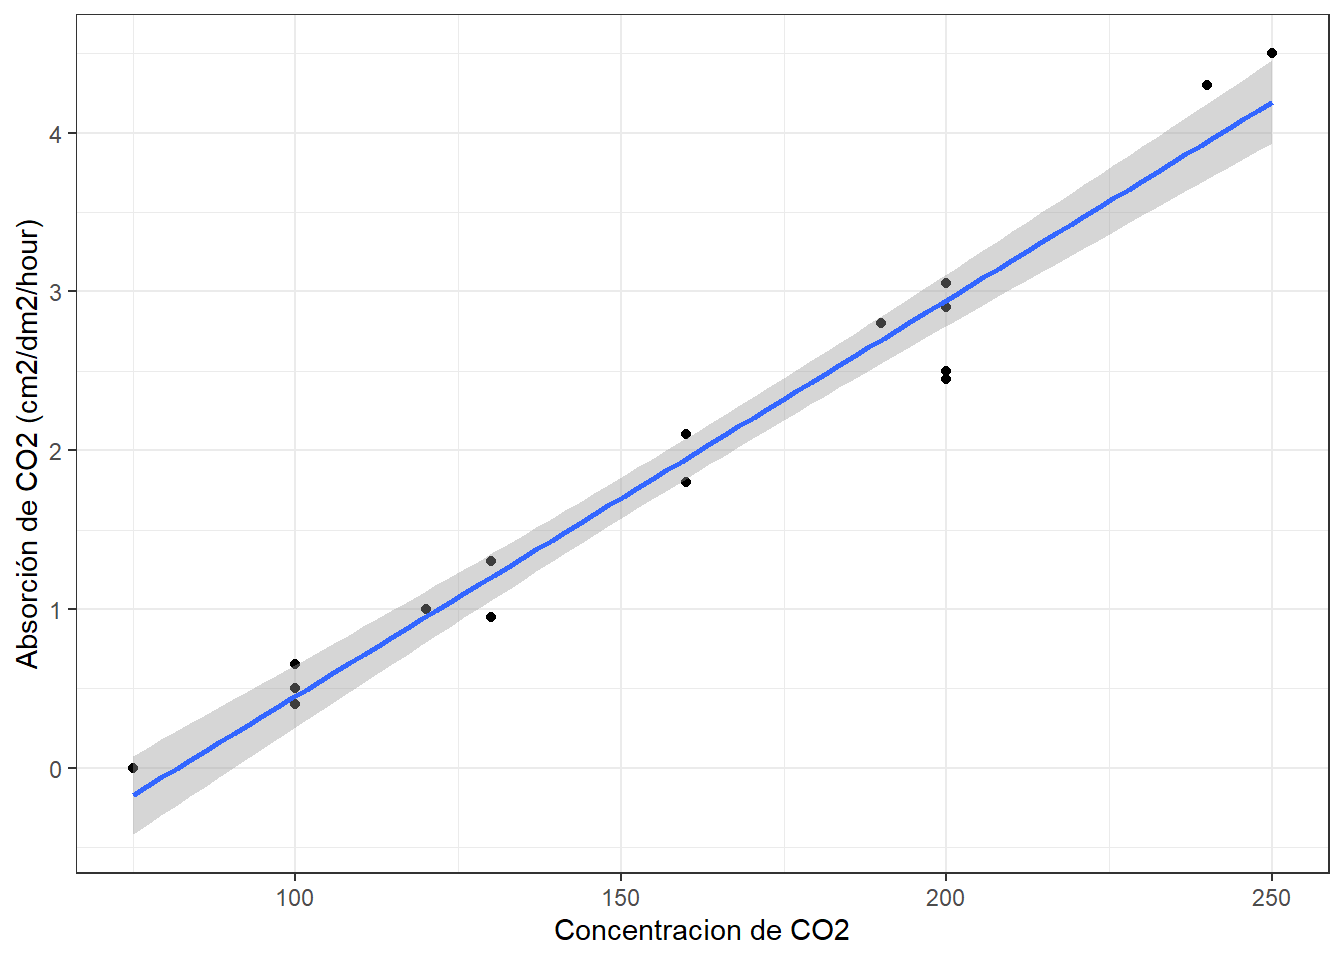
\includegraphics{07-lab_files/figure-latex/unnamed-chunk-10-1.pdf}

\hypertarget{expresar-la-hipuxf3tesis-de-investigaciuxf3n-1}{%
\subsection{Expresar la hipótesis de investigación}\label{expresar-la-hipuxf3tesis-de-investigaciuxf3n-1}}

El siguiente paso contempla expresar la pregunta o hipótesis de investigación en al menos dos hipótesis estadísticas contrastantes: nuestra hipótesis nula \(H_0\) y nuestra hipótesis alternativa \(H_A\).

Para evaluar estadísticamente la relación entre ambas variables, podemos establecer el siguiente par de hipótesis:

\[
H_0: \text{No hay relación entre las variables Uso de Herbicida y Estado de Salud}\\
H_a: \text{Hay relación entre las variables}
\]

El objetivo es testear la veracidad de la \(H_0\). Para poner a prueba la \(H_0\), es necesario realizar una prueba estadística.

\hypertarget{calculemos-chi2-y-el-p-value-1}{%
\subsection{\texorpdfstring{Calculemos \(\chi^2\) y el p-value}{Calculemos \textbackslash chi\^{}2 y el p-value}}\label{calculemos-chi2-y-el-p-value-1}}

Las diferentes pruebas de hipótesis utilizan diferentes estadísticos de prueba según la distribución de probabilidad asumida en la \(H_0\). En el caso de la prueba de independencia de \(\chi^2\) , el estadístico de la prueba se llamará estadístico de \(\chi^2\).

Calculemos el estadístico de \(\chi^2\) y el \texttt{p-valor} para una prueba de independencia de utilizando las variables categóricas estado de salud y uso de herbicida:

\begin{Shaded}
\begin{Highlighting}[]
\NormalTok{res_ind <-}\StringTok{ }\KeywordTok{chisq.test}\NormalTok{(data}\OperatorTok{$}\NormalTok{Uso_herbicida, data}\OperatorTok{$}\NormalTok{Estado_salud)}
\NormalTok{res_ind}
\end{Highlighting}
\end{Shaded}

\begin{verbatim}
## 
##  Pearson's Chi-squared test with Yates' continuity correction
## 
## data:  data$Uso_herbicida and data$Estado_salud
## X-squared = 6.4172, df = 1, p-value = 0.0113
\end{verbatim}

Nuestro estadistico \(\chi^2\) es igual a 6.4172, nuestros grados de libertad son 1 y el valor de probabilidad es de 0.0113

\hypertarget{conclusion-del-test}{%
\subsection{Conclusion del test}\label{conclusion-del-test}}

Se rechaza la hipotesis nula. Por lo tanto, tenemos evidencia para sugerir que hay relación entre las variables Uso de Herbicida y Estado de Salud

\hypertarget{estaduxedstica-inferencial-regresiuxf3n-lineal-y-correlaciuxf3n}{%
\chapter{Estadística inferencial: Regresión lineal y correlación}\label{estaduxedstica-inferencial-regresiuxf3n-lineal-y-correlaciuxf3n}}

Antes de comenzar con este práctico es importante tomarnos un tiempo para recordar que la estadística comienza con un problema, continúa con la toma de datos, sigue con la inspección y visualización de los datos y termina con el análisis de los mismos. Esto nos permitirá sacar conclusiones fundamentadas sobre nuestro problema inicial.

En el presente curso hemos establecido una receta de trabajo al momento de realizar inferencias estadísticas:

\begin{itemize}
\item
  \textbf{Paso 1: Graficar nuestros datos.} El objetivo es evaluar posibles tendencias en nuestros datos.
\item
  \textbf{Paso 2: Definir la hipótesis que queremos poner a prueba.} Debemos establecer la hipótesis nula y la(s) alternativa(s).
\item
  \textbf{Paso 3: Transformar la hipótesis en un modelo (prueba) estadístico.}El modelo estará determinado por nuestras variables (importante diferenciar entre variables continuas y categóricas).
\item
  \textbf{Paso 4: Evaluar los supuestos del modelo.} Es relevante para saber si podemos (o no) utilizar métodos paramétricos.
\item
  \textbf{Paso 5: Interpretar los resultados del modelo.} Debemos evaluar el valor de probabilidad asociado a la prueba estadística.
\end{itemize}

\hypertarget{modelos-lineales-generales}{%
\section{Modelos Lineales generales}\label{modelos-lineales-generales}}

En muchas oportunidades estaremos interesados en saber como el comportamiento de una variable, o un conjunto de variables, impacta sobre otra. El objetivo es entender el grado de asociatividad y/o la posible relación funcional entre las variables.

Los modelos lineales generales describen una variable respuesta (\(y\)) en términos de todos sus factores contribuyentes (\(xβ\)) en una combinación lineal, mientras que también incorpora el aporte de error (\(e\)).

\begin{equation} 
  Y  = β_{0} + β_{1}X_{1} + e 
  \label{eq:ecuacion1}
\end{equation}

Esta clase de modelos estadísticos incluye la regresión lineal, regresión múltiple, ANOVA y ANCOVA.

En R, todos los análisis univariados (una variable respuesta) de este tipo se ajustan utilizando una única función \texttt{lm()}.

El análisis de regresión lineal se usa para explicar o modelar la relación entre una variable continua \texttt{Y}, llamada variable respuesta o variable dependiente, y una variable continua \texttt{X\textasciitilde{}1\textasciitilde{}}, llamada variable explicativa o independiente. Cuando hay más de una variable continua explicativa (X\textsubscript{1}, X\textsubscript{2},\ldots{} X\textsubscript{p}) el análisis se denomina \textbf{regresión múltiple}.

Si la variable explicativa es categórica en vez de continua, entonces el análisis a realizar es un \textbf{ANOVA} (en inglés) o análisis de varianza de 1-vía. Cuando hay dos variables categóricas explicativas, el análisis se denomina \textbf{análisis de varianza de 2-vías}. Es fácil imaginar como se llamará el análisis en caso de tener 3 o más variables categóricas explicativas, ¿no?.

Por ultimo, es posible que en un mismo análisis aparezcan variables explicativas tanto continuas como categóricas, y en este caso el análisis pasaría a denominarse análisis de \textbf{covarianza} o \textbf{ANCOVA}.

\hypertarget{correlaciuxf3n-producto-momento-de-pearson}{%
\subsection{Correlación producto-momento de Pearson}\label{correlaciuxf3n-producto-momento-de-pearson}}

Antes de comenzar la construcción de modelos lineales complejos, es importante observar la relación de datos para comprender cómo interactúan las diferentes variables. La correlación producto-momento de Pearson (para simplificarnos la vida hablaremos de correlación de Pearson) determina si existe asociación entre dos variables continuas. Dicho de otra forma, la correlación de Pearson analiza si dos variables continuas cambian de forma simultánea (están relacionadas).

El coeficiente de correlación de Pearson (r) es una medida de la fuerza de una asociación lineal entre dos variables continuas. El coeficiente de correlación de Pearson puede tomar un rango de valores de +1 a -1. Un valor de 0 indica que no hay asociación entre las dos variables. Un valor mayor que 0 indica una asociación positiva; es decir, a medida que aumenta el valor de una variable, también lo hace el valor de la otra variable. Un valor menor que 0 indica una asociación negativa; es decir, a medida que aumenta el valor de una variable, el valor de la otra variable disminuye.

Es importante destacar que la correlación de Pearson no tiene en cuenta si una variable se ha clasificado como una dependiente o independiente. Trata a todas las variables por igual. Incluso, las variables pueden estar medidas en diferentes unidades.

Empleamos la correlación de Pearson para determinar si dos variables cambian de forma independiente (H\textsubscript{0}) o entonces, de forma alternativa, de forma conjunta (H\textsubscript{1}).

Recuerden importar la nueva base de datos data.csv!

Trabajaremos con la superficie de territorio plantada con Vid y con Olivo. Recordemos que nunca debemos comenzar un análisis estadístico con una prueba estadística, siempre debemos comenzar con una figura de nuestros datos!!!

\backmatter
  \bibliography{book.bib}

\end{document}
